\documentclass[preprint]{aastex}
\usepackage{graphicx}

\newcommand{\code}[1]{\texttt{#1}}
\newcommand{\Fig}[1]{Fig.~\ref{#1}}
\newcommand{\Sec}[1]{Sec.~\ref{#1}}
\newcommand{\Table}[1]{Table~\ref{#1}}
\newcommand{\ticket}[1]{ticket \code{\##1}}
\newcommand{\by}{$\times$}

\shorttitle{LSST Data Challenge 3a}
\shortauthors{Axelrod, et al.}

\DeclareGraphicsExtensions{.pdf,.jpg,.png,.eps}

\newcommand{\XXX}[1]{{\bf XXX #1}}      % Please use this for anything that needs to be written;
                                        % we can comment the definition and find all the \XXXs

\newcommand{\RHL}[1]{{\bf RHL: #1\qquad}}     % A comment from RHL.  None should remain in the final document!

% -- a @%< hack to redefine placement of abstract in \maketitle
\makeatletter
\def\@maketitle{%
 \newpage
 \begingroup
  \let\footnote\thanks
  \let\email\make@authoremail
  \let\affil\make@affil
  \let\altaffilmark\make@altaffilmark
  \let\altaffiltext\make@altaffiltext
  \let\and\make@and
  \@title
  \@author
  \@date
  \par
  %\@abstract
  \@ifxundefined\keyword@list{}{%
   \expandafter\@keywords
   \expandafter{\keyword@list}%
  }%
 \endgroup
 \clearpage
}%
\makeatother


\begin{document}

\title{LSST Data Challenge 3a}


% -- Author/Affiliation information
\author{Tim Axelrod, Robyn Allsman, Jeff Kantor, 
        Francesco Pierfederici}
\affil{LSST Corporation}

\and\author{Serge Monkewicz, Russ Laher, Deborah Levine, Vince
  Mannings, Jeonghee Rho, Peregrine McGehee}
\affil{NASA Infrared Processing and Analysis Center}

\and\author{Greg Daues, David Gehrig, Steve Pietrowicz, Raymond Plante}
\affil{National Center for Supercomputing Applications}

\and\author{Jacek Becla, Kian-Tat Lim}
\affil{SLAC National Accelerator Laboratory}

\and\author{Andrew Becker, Andrew Connolly, Russell Owen, Nicole Silvestri}
\affil{University of Washington}

\and\author{Steven Bickerton, Robert H. Lupton, Fergal Mullally}
\affil{Princeton University}

\and\author{Richard A. Shaw}
\affil{National Optical Astronomy Observatory}

\begin{centering}
\textbf{ABSTRACT}

\begin{quotation}\noindent%
This report describes the third in a series of formal prototypes of
the LSST Data Management System referred to as Data Challenge 3a (DC3a).
The focus of this data challenge is to enhance both the science applications
and the software infrastructure supporting those applications to add
increased functionality as guided by our analysis of the results of DC2. 
We enumerate the goals and metrics for DC3a, summarize the architecture
of the DC3a pipeline system, and review the science application and middleware
components that make up the system.  Finally, we present the results
of executing DC3a on data from the CFHT Legacy Survey and simulated
exposures created for LSST Data Management, and highlight the important 
conclusions that will be used as input into the next data challenge.  
\end{quotation}
\end{centering}

\tableofcontents

% -- section 0
\pagebreak
\section*{Executive Summary}
\addcontentsline{toc}{section}{Executive Summary}

\subsubsection*{Introduction}

Data Challenge 3 (DC3) is the third in a series of prototypes of the
LSST Data Management System (DMS). Through these data challenges, we
seek to prototype and validate proposed solutions to the most 
challenging technical problems to building a
DMS that meets the LSST science goals.

In Data Challenge 1 (DC1), we focused on the DMS middleware design
for supporting nightly processing; this software scaffolding ---
the \textit{pipeline framework} --- modeled the infrastructure
necessary to support science algorithms but did not actually execute
them, using instead \textit{resource consumers}, which simulated the
expected computational node of the algorithms but produced no useable
science output.  In Data Challenge 2 (DC2), we replaced the resource
consumers with real implementations for the most challenging aspects of
the Alert Production, focusing on image processing. We also updated the pipeline
framework as development of the scientific algorithms revealed
new framework requirements.

The scope of DC3 is significantly larger than that of the previous
data challenges, including both a more capable implementation of the
Alert Production and a first prototype implementation of the Data
Release Production.  Because of the large scope of DC3, it is
divided into two phases, DC3a and b.  DC3a, the subject of this report, included only the Alert
Production capabilities, while DC3b adds the Data Release Production.
Other aspects of DC3a included improvements to the application framework
and middleware, along with the following new capabilities: the
Instrument Signature Removal (ISR) pipeline, World Coordinate System
(WCS) determination within the Image Characterization (IC) pipeline,
and an initial SDQA system. Finally, in DC3a significant improvements were 
made in the execution speed of the science applications,  and incremental improvements were 
made in science data quality and within the software build system.

\subsubsection*{Productions Runs Performed and Scalability}

As in DC2, the astronomical images we used as input were from the CFHT-LS
Deep Survey fields D3 and D4.  We also executed some but not all pipeline 
stages using images from the LSST simulated data collections, SimWide and
SimDeep, and these runs were instrumental in understanding and
correcting processing problems.

After initial short runs for purposes of debugging, 
we executed larger-scale DC3a production runs on clusters at
NCSA.  For final analysis of data quality and processing performance,
we have concentrated on two production runs on the NCSA LSST
development cluster (referred to by their run
identifiers, \texttt{rlp1233} and \texttt{rlp1234}. These runs used
identical versions of the software and were configured identically, but
processing a different set of 31 amplifiers in the focal plane for 85
visits to the CFHT-LS D3 field.  To explore the scalability of
the pipelines, we also executed runs of the image processing pipeline
on the NCSA cluster Abe.  These runs were performed across 36 8-core
nodes, processing the entire 288-amplifier focal plane for CFHT-LS
simultaneously.  (Some of the supporting software services, such as
the event broker and the database, remained on the NCSA LSST cluster.)

These runs showed that the pipelines scaled reasonably well to the
level of 10\% of the actual LSST image size, although running at this scale did reveal some additional
configuration requirements for the events broker and the MySQL
database.  To run on Abe, we integrated grid-based technologies
(including grid-based job management using Condor-G) into our the
pipeline orchestration layer.  While short of our goal of 15\% of the actual LSST image size,
we elected to close out DC3a at this level in order to expedite completing this report.
We expect to complete runs up to the 15\% level before PDR.

\begin{table}[ht]
\centering
\caption{Summary of Production Runs analyzed in this report
\label{tbl:runsummary}}
\vspace{\baselineskip}
\begin{tabular}{rccccc}
\hline\hline
          &         &       & \multicolumn{3}{c}{Images Processed: Num/Size} \\
runId     & nVisits & nAmps & Raw Images & Ancil. Images & Output Images \\ \hline
rlp1233   & 85      & 31  & 5146/24 GB    & 88/13 GB       & 60525/240 GB \\ 
rlp1234   & 85      & 31  & 5146/24 GB    & 88/13 GB       & 60525/240 GB \\ 
rlpabe041 & 12      & 288 & 3456/33 GB    & 15/2 GB        & 79368/313 GB \\ \hline
Total     & ---     & 250 & 13748/81 GB   & 191/28 GB      & 2000418/793 GB \\ \hline
\end{tabular}
\end{table}

Finally, in DCs 1, 2, and 3a, the availability of computational and storage resources has not
significantly impacted the scaling tests possible.  Since the Data Release Production will 
involve significantly larger data volumes and computational load, the volume
and performance achievable in DC3b will be limited by the available resources.

\subsubsection*{Algorithm/Application Performance}

While the total processing time per
visit is longer than in DC2, we note that DC3a does significantly more processing,
including additional caching of intermediate results that would not be
necessary in production mode.  When we examined the common stages of
processing in DC2 and DC3a, we saw large improvements across the
board, along with a much lower variation in processing times over
different data.  The most expensive stage, image subtraction, saw a
2-fold improvement over DC2; subsequent experiments showed tuning
configuration parameters increased that factor to 3.

While the improvements are significant and on a pace 
with our expectations for this stage of the project, 
we are still not meeting the full latency and throughput
requirements of the operational DMS by approximately a factor of 4.  As we do not expect 
this gap to be closed significantly by basic improvements in cluster hardware, 
we are targeting both algorithmic
improvements and alternative hardware architectures (GPUs) in future DCs.

\begin{table}[ht]
\begin{center}
\caption{Average Processing Times Per Visit
\label{ex:tbl:visitstats}}
\vspace{\baselineskip}
\begin{tabular}{ l | c | c }
\hline\hline
          & Total Processing Time, corrected
          & Application Processing Time \\ 
Pipeline  & average $\pm$  $3\sigma$ (s) & average $\pm$ $3\sigma$ (s) \\ \hline
IPSD      & 264.7 $\pm$ 20.2 & 264.1 $\pm$ 20.1  \\ 
nightmops & 10.6  $\pm$  4.4 & 10.4 $\pm$  4.4  \\ 
ap        & 1.4   $\pm$  0.7 & 1.2 $\pm$  0.7  \\ \hline
\hline
\end{tabular}

\end{center}
\end{table}

Finally, the results continue to show that the overhead 
added by the  pipeline framework is minimal.
The comparison of the runs also revealed technology-, platform-, and configuration-specific results for stages
handling I/O, particularly when we considered filesystem and database
I/O separately. In DC3b, we will spend more effort developing better I/O
strategies, optimizing the use of parallel filesystems and deploying distributed databases.  

\subsubsection*{Science Data Quality}
As in DC1 and DC2, DC3a did not focus on major improvement to science data quality.  
In DC3b this will be a major focus, and we anticipate significant involvement from
members of the LSST Science Collaborations in evaluating data quality and algorithm accuracy
and efficiency.

Nevertheless, we employed both algorithm developers and independent
 (non-DC) scientists from IPAC
to evaluate the science data quality of DC3a in three areas that are
judged to be the most demanding for the software system to meet, 
and are each directly related to science requirements:
\begin{itemize}
\item WCS accuracy was acceptable in 98\% of images processed, with median errors of 40 milli-arcsec.
\item The noise level away from bright stars in difference images with acceptable WCS is near 1.0, as expected.
\item The noise level near bright stars in difference images with acceptable WCS is near 20 (unacceptable), and this will be addressed in DC3b by refining the kernel basis functions chosen for image subtraction.
\item Difference image lightcurve quality was adversely affected by residuals around bright stars and will be re-evaluated once the basis functions are addressed.
\end{itemize}

\subsubsection*{Project Management}
A comparison between DC2 and DC3a reveals the following productivity statistics:
\begin{itemize}
\item 28 staff at 30\% time average in DC3a vs.~19 staff at 50\% time average in DC2;
\item 9 months estimated/14 months elapsed time in DC3a vs.~10 months estimated/12 months elapsed time in DC2;
\item 107k lines of code produced (c++, python, SQL, java, scripts) in DC3a vs.~90k in DC2.
\end{itemize}

As can be seen from the above, in DC3a there was  a significant schedule overrun (50\%).
The team was very late in establishing the final scope 
and developing resource leveled plans. The reasons for this include a larger team but
 lower per-person involvement than in DC2.
This caused more and longer periods where parts of the team were blocked
waiting for other parts to complete, as well as requiring more time to be spent 
on coordination between locations.
In addition, some major items were significantly underestimated (e.g. reworking of the core image classes
in the Application Framework) and should have been better specified early on.
Changes are being made to the team organization and process to improve this in future DCs.


\pagebreak

% -- Section 1
% section 1: Introduction

\section{Introduction}

Data Challenge 3 (DC3) is the third in a series of prototypes of the
LSST Data Management System (DMS). Through these data challenges, we
seek to identify the most challenging technical problems to building a
DMS that meets the LSST science goals. We prototype specific solutions
to these challenges with the expectation that by the start of the
construction phase of the telescope, we will have a well-defined plan
for how to build a DMS that can perform at the level needed by first
light. Despite the prototyping nature of the data challenges, we are
not producing throwaway code; rather, we expect that the software we
produce in the data challenges will serve as the foundation for the
DMS that will be completed during the construction phase.  In Data
Challenge 2 (DC2; Axelrod {\it et al.} 2008), we focused on
demonstrating the use of astronomical algorithms for nightly
processing in an LSST processing framework.  The scope of DC3 is
significantly larger, including both a more capable implementation of
the Alert Production and a first prototype implementation of the Data
Release Production.

Because of the large scope of DC3, we have divided it into two phases,
DC3a and b.  DC3a includes only the Alert Production capabilities,
while DC3b adds the Data Release Production.  This report describes
the results of DC3a only. We enumerate our goals, summarize the
implementation, and report on what we've learned from it.

\subsection{Goals of DC3a}

The goals of DC3a were in part an outcome of the DC2 post-mortem
analysis.  The DC2 report (Axelrod {\it et al.} 2008) listed several
areas where improvement was needed, and these have largely been
incorporated into the DC3a goals, which are as follows:

\begin{itemize}
\item Application Framework improvements;
\item Middleware improvements;
\item Implement the Instrument Signature Removal (ISR) pipeline
\item Implement the Image Characterization Pipeline (ICP), in
  particular the determination of the WCS;
\item Implement an initial SDQA system;
\item Improve the science quality of the difference images and
  resulting catalogs;
\item Improve the execution speed to a level that gives confidence in
  scaling to the full LSST; and
\item Improve the capabilities of the software build system.
\end{itemize}

We address our success in achieving these goals in subsequent sections
of this report, and summarize in \Sec{sec:results}.


% -- Section 2
% section 2: Components

\section{Components}  \label{sec:components}

The DC3a Alert Production is accomplished through a set of
\textit{pipelines} that work together, which collectively we refer to
as a \textit{production}.  A \textit{production run} is a particular
instantiation and execution of those pipelines that produces a
collection of data products. In the case of alert production these include
the calibrated images, subtracted images, and a catalog of detected objects.  A
\textit{pipeline} itself is a series of processing steps (called
\textit{stages}) which are cyclically applied to a sequence of data
chunks.  Since the alert production is meant to run in real time on data
coming from the telescope, the chunks of data to be processed are 
 \textit{visits}, in which each visit is comprised of two
15-second exposures of the same field in the sky.  Each visit,
generally, covers a different field in the sky and/or observing filter.    
Figure \ref{fig:dc3apipes} diagrams major components of the processing flow in DC3a;
figure \ref{fig:lsstpipes} shows for comparison the baseline design for processing 
flow in the fully implemented LSST.

Building on the design from DC2, the Alert Production is comprised of
three pipelines: 

\begin{itemize}

\item The \textit{image processing and source detection} (IPSD)
  pipeline takes as input the raw exposure images along with the
  related calibration data, produces calibrated images, and then
  differences them from template images of the same field.  It then
  produces a catalog of the light sources found within those
  difference images. DC3a added image signature removal to this
  pipeline, along with the paradigm of processing both exposures that
  make up the visit and use them to discriminate against cosmic ray
  defects.

\item The \textit{Night Moving Object Processing System} pipeline
  (NightMOPS) takes time and coordinate information from the exposure
  and creates a catalog of known solar system objects expected to be
  within the exposure FOV. It operates in parallel with the IPSD
  pipeline.

\item The \textit{association pipeline} (AP) then correlates the
  sources found by the IPSD with known objects --- either fixed
  objects or objects expected by NightMOPS to be within the FOV --- to
  determine whether new sources have been detected.

\begin{figure}[t]
\begin{center}
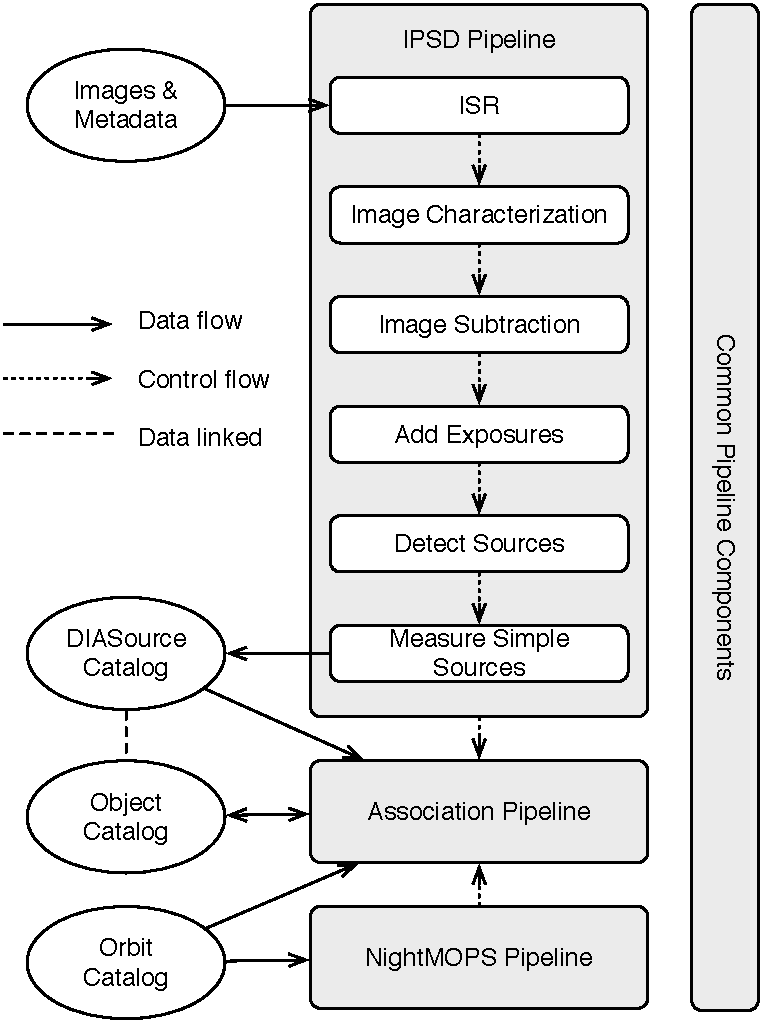
\includegraphics[width=3in]{images/DC3aNightly.pdf}
\caption{Processing flow in DC3a. Three pipelines (IPSD, Association, and
NightMOPS) are supported by a common infrastructure.  
\label{fig:dc3apipes}}
\end{center}
\end{figure}

\begin{figure}[t]
\begin{center}
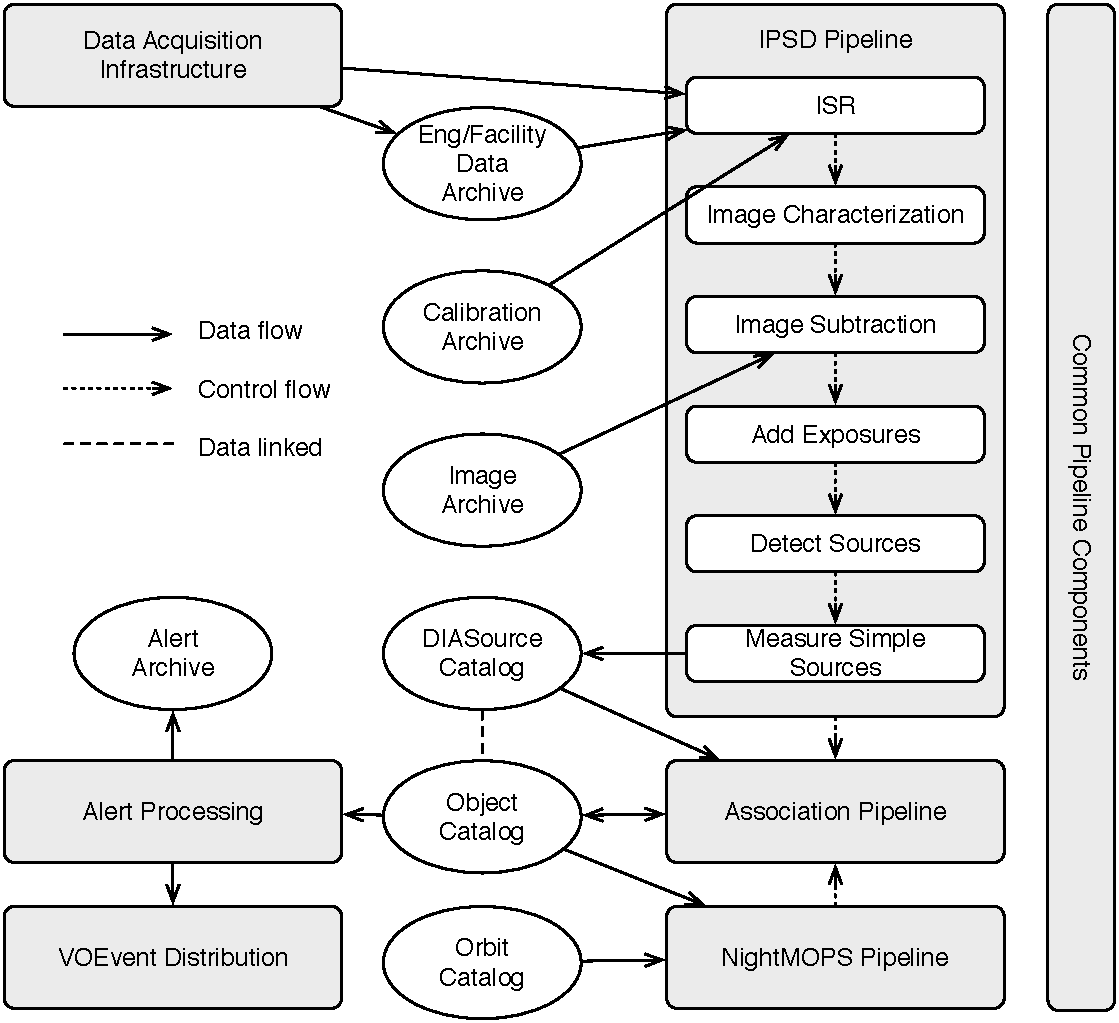
\includegraphics[width=4.5in]{images/LSSTpipes.pdf}
\caption{Baseline design for nightly image processing flow for LSST; DC3a represents
a subset of this design.  
\label{fig:lsstpipes}}
\end{center}
\end{figure}


\end{itemize}

A pipeline can process data in highly parallelized manner; in general,
a pipeline will use a consistent model of data parallelism, in which a
parallel process (a \textit{slice}) will operate on the same logical
portion of the input dataset throughout all the pipeline stages.  For
example, each slice in the IPSD pipeline processes a different
amplifier segment of a CCD that comprises the focal plane.  The
NightMOPS pipeline distributes the known objects in its catalogue
across its slices.  

The three pipelines run simultaneously on different machines but are
loosely coupled via event-based communication.  In particular, the
IPSD and NightMOPS pipelines will process the next visit when they
receive an external event message indicating that a new visit is
available for processing.  These pipelines each emit an event message
when they have finished processing a visit.  These events are picked
up by the AP pipeline as a signal that there are new detections in the
database to be associated with known objects.  The routing of these
event messages between pipelines is facilited by an \textit{event
broker} (which runs as a separate process).  

Events are also used for collecting logging messages from all of the
processes that make up the pipelines.  A special \textit{event
monitor} program collects these messages and loads them into the
database.  

The whole production is configured via a set of human-readable
\textit{policy files} which provide values for parameters that
configure the behavior of the various pipeline components.  In
particular, a production-level policy defines the pipelines that
make up the production along with the properties of the platforms that
they will run on.  Pipeline-level policies define the stages that make
up each pipeline along with details for setting up the pipeline for
execution.  Each stage also has a policy that sets various parameters
used by algorithms that will be applied to the data.  

Data Products come in two forms: FITS images and records into a
database.  A shared MySQL database is used for the latter.  In
particular, insert into and retrieval from the database is the main
mechanism for passing object and source information betweeen
pipelines.  

\subsection{Overview of Processing Flow}

In this section, we take a closer look how the different software
components work together to process the sequence of visits that come
from the telescope.  

\subsubsection{Middleware for Launching and Managing Pipelines} 
\label{sec:orcaintro}

The \textit{orchestration layer} is responsible for configuring,
preparing, launching, and monitoring the pipelines that make up a
production.  In general, each pipeline can be deployed on a different
platform, so the orchestration layer must be able to adapt to
different platforms and operate remotely.  The layer is implemented
via the \texttt{ctrl\_orca} software package (short for
``Control-Orchestration''; see section \ref{sec:PipelineOrchestration})
and initiated via its \texttt{orca.py} launch script.  This basic
inputs to this script includes a production-level policy file
(\texttt{dc3pipe.paf}) which contains pointers to all the other policy
files needed to configure the pipelines.  Another important input is
the \textit{run identifier} (or ``run-ID'', for short) which is a
short name that identifies a particular instantiation of the pipelines
and the overall collection of data products they will produce.  When
executed, the script will:  

\begin{itemize}
\item Create working directories on the target platforms for input and
  output data, policy files, and log files,
\item Initialize the database tables to be used by the pipelines, 
\item Deploy all needed policy files and launch scripts onto the
  target platforms,
\item Set the necessary software environment, and 
\item Remotely execute each platform launch script.
\end{itemize}

For DC3a, the \texttt{orca.py} script was executed through another
script called \texttt{launchDC3a.py} from the \texttt{ctrl\_dc3pipe}
package.  This script handles setup that is specific to DC3a.  In
particular, after executing the \texttt{orca.py} script, it runs
another script that creates and emits the ``data-is-available'' events
that trigger the IPSD and NightMOPS pipelines to start processing.
(During actual production operation of the observatory, these events
would be generated by the observatory control software.)  These events
are emitted at a specified cadence to simulate retrieval of data from
the telescope.  

\begin{figure}[t]
\begin{center}
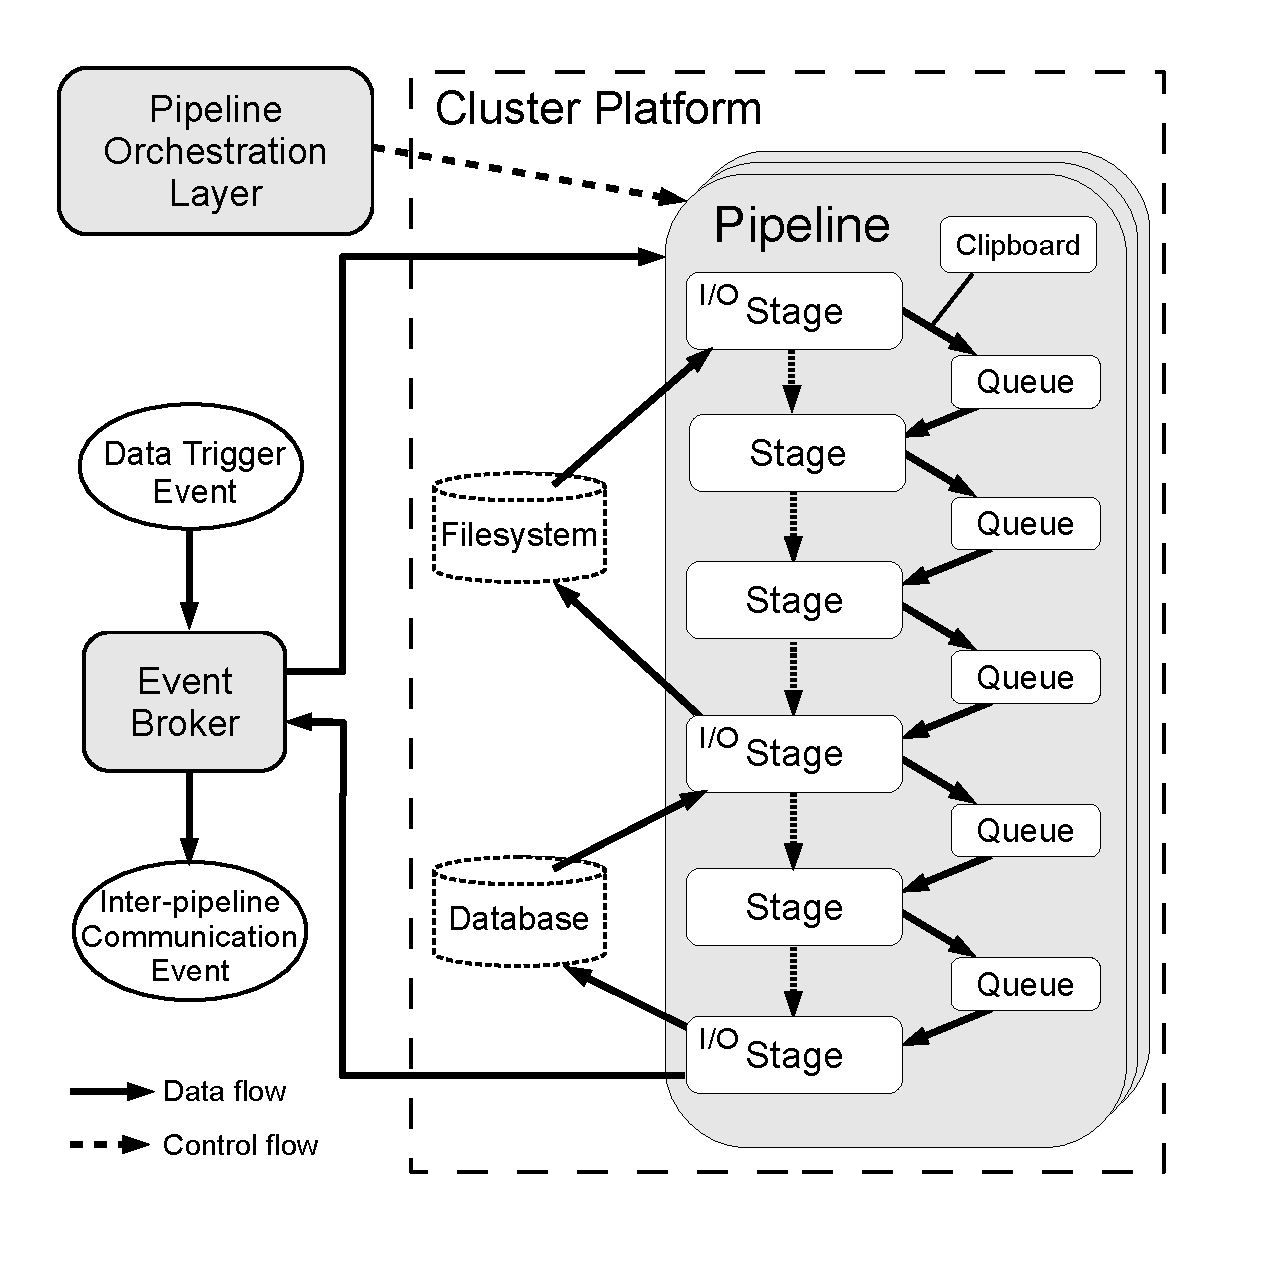
\includegraphics[height=4.0in,bb=25 45 562 583]{images/pex.pdf}
\caption{The generic pipeline framework. The pipeline orchestration
  layer launches the pipeline on a remote cluster, resulting in
  multiple parallel pipeline processes across the cluster machines.
  Processing starts when the pipeline receives a data trigger event
  via the event broker, and data and control pass through the stages.
  Some of the stages are dedicated to I/O.  The last stage can issue
  an event to trigger another pipeline to take over the processing of
  the data.
\label{fig:pex}}
\end{center}
\end{figure}

The ``science view'' of what each pipeline does in response to these
events is summarized in the subsequent sections below; however, these
actions are facilitated by the \textit{pipeline harness}, the
application container that hosts the application code which applies
the specific scientific algorithms to the data, as illustrated in
Fig. \ref{fig:pex}.  The harness runs a pipeline: it is responsible
for capturing events and making the data they contain available to the
application.  It also manages the flow of execution, executing each
stage in sequence, passing data between them, and start the sequence
over again when all the stages are done processing a chunk of data.  

Additional details of how the harness does its work can be found in
section \ref{sec:harness} and more so in the DC2 Report.  For the
discussion below, it is useful to introduce some operational concepts
that are part of the harness framework.  First, we explicitly
segregate processing into three different types of stages:  science
stages (that apply science processing algorithms to the data), I/O
stages (that read in or write out data), and miscellaneous
book-keeping stages.  This is important for our performance analysis
as we want to be able explicitly separate the effects, say, I/O from
the science algorithms.  All I/O operations, be they on files in a
filesystem or operations on a database, go through an abstract
layer referred to as \textit{persistence}.  In particular, to
\textit{persist} some data is to use the persistence layer to save a
copy of the data on disk, possibly in a database.  \textit{Loading} is to
read the data from disk and into objects in memory.  I/O is handled
through a generic stage implementation provided by the
\texttt{pex\_harness} package which can be configured via a policy to
read or write any data available via the persistence layer.  

Data objects are moved through stages attached to a \textit{clipboard}
object and transferred via \textit{queues} that connect the stages
(see fig. \ref{fig:pex}): any stage that wants to share data with
subsequent stages can ``post'' it to the clipboard and sending it to
its output queue.  In the current implementation, the clipboard is an
object in memory shared by all the stages; thus, no I/O, network
communication, or other data copying is involved in the transfer.

\subsubsection{Image Processing and Source Detection (IPSD)}

The IPSD pipeline processes images in pairs: two exposures, designated
0 and 1, are considered to have been taken consecutively with the same
field of view at essentially the same time. This pairing of exposures
allows for the detection of cosmic rays appearing in one exposure but
not the other.

The IPSD performs the following tasks, in sequence:

\begin{itemize}

\item Information is read in identifying the exposures to be processed, and 
links are created in the file system from the working directory to the input
images.

\item For image 0 of the pair, metadata in the FITS file header is read in, 
giving the exposure time, location of the field of view, and similar information, 
which is then posted to the clipboard.

\item Given this information, the calibration products associated with that
exposure are identified by lookup. Calibration products include darks,
flats, bias, and scatter exposures associated with a given camera run.

\item These calibration products are then used to perform instrument
signature removal (ISR) on the raw exposure, resulting in a calibrated image.

\item Source detection is then performed on calibrated image, giving source
information needed later for determining the WCS coordinates of the
exposure.

\item The point spread function (PSF) of the exposure is determined.

\item The second image of the pair is read in and also goes through ISR.

\item WCS of the exposures is determined.

\item The calibrated exposures are then persisted.

\item A template image representing the ideal expected exposure is
created. When processing CHFT-LS images, these templates are 
resampled from stacked images provided by the CHFT-LS survey.

\item Calibrated images 0 and 1 are subtracted from the template
image, and the difference images created are persisted.

\item These difference images are added together. Source detection
and measurement is then performed. The resulting DIASources are then
separately measured in each exposure individually.  Based on
comparison of the two sets of measurements, classification
flags are set and persisted with the DIASources in the science database.

\item The association pipeline is signaled through the events broker
that the processing of the image pair is complete and that the source
data is ready for the association process.

\item SDQA data from the exposure is persisted.

\end{itemize}

\subsubsection{Night Moving Object Processing System (MOPS)}

The MOPS pipeline performs the following tasks, in sequence:

\begin{itemize}

\item Given the required field of view and time of exposure, MOPS predicts the positions 
of known moving objects in the field.

\item These positions are recorded into the database.

\item MOPS then signals the association pipeline, through the events
broker, that its predictions are available.

\end{itemize}

\subsubsection{Association Pipeline (AP)}

The association pipeline performs the following tasks, in sequence:

\begin{itemize}

\item The pipeline awaits signals from the event broker that
both the IPSD and MOPS pipelines have completed their computations
on a given pair of exposures.

\item New source detections from the DIASource catalog are loaded 
into memory.

\item These detections are matched against known, fixed objects.
Matches are recorded into the database.

\item The MOPS predictions for known moving objects are loaded 
into memory, and the new source detections are matched against
these predictions. Again, matches are recorded in the database.

\item New sources are then used to update the catalog of known
objects.

\end{itemize}

\subsection{Hardware Deployment}

\subsubsection{The NCSA LSST Cluster}

Most of the DC3a preliminary and production runs were performed on a dedicated 
ten-nodes Dell Server Xeon cluster hosted at NCSA. This heterogenous cluster 
consists of two Xeon 3.6 GHz single dual-core nodes, two Xeon 3.6 Ghz dual
dual-core nodes, and six Xeon 2.0 Ghz dual quad-core nodes. It uses a
gigabit ethernet interface.

This cluster was built for DC2 and the DC2 runs were performed there; for DC3, 
the cluster was upgraded from 32-bit Red Hat Enterprise Linux 4 to 64-bit
Red Hat Enterprise Linux 5. Each cluster node has 4 GB memory, with the exception
of \texttt{lsst10}, which has 16 GB. Each node has from 20 to 60 GB of local disk,
along with 15 TB of disk storage shared among nodes using the NFS shared file system.
As part of DC3a, we installed the Lustre parallel file system to increase I/O 
throughput. We were not, however, able to stabilize the Lustre installation
sufficiently to use it for production runs on the NCSA cluster, as planned.

\subsubsection{NCSA Abe}

For purposes of testing the scalability of the pipelines, additional runs were
performed on a larger cluster, Abe, hosted at NCSA. Abe consists of 1200
dual quad-core Xeon 2.33 GHz processors; for the LSST runs we used 36 of these 
nodes, for a total of 288 cores, sufficient to process an entire focal plane 
for the CHFT-LS images. Each core has 1 GB of memory, and shared access
to 100 TB of disk storage as managed using Lustre.

Abe job runs were coordinated using the Condor-G jobs management system.
The events broker and database were not moved to Abe during these runs;
they remained on the LSST cluster.


% -- Section 3
% section 3: Software Development Practices

\section{Software Development Practices}

\subsection{UML Modeling}

\subsection{Software Development Environment}





% -- Section 4
% section 4: Input Data

\section{Input Data}


\subsection{CFHT-LS Deep Survey Data}

32 CCDs.

\subsubsection{Science Data Products}

The ``raw'' archival science data obtained from CFHT have  gone through
a modicum of pre--processing by the CFHT {\tt ELIXIR}
pipeline\footnote{\url{http://cfht.hawaii.edu/Instruments/Imaging/MegaPrime/rawdata.html}}.
In particular, the two amplifier readouts were spliced back together
into 2112 by 4644 pixel images corresponding to a single CCD.  To prepare the data for DC3a processing, we need
to undo this operation to some degree, while still maintaining
consistency between the valid data sections, overscan regions, and
approximate Wcs information in the image headers.

For DC3a processing, we divided each of the 32 CCD images into 8 images
that are approximately the anticipated size of LSST amplifier images.
Synthesized amplifier images 0-3 come from CFHT image subsection {\tt
[0:1056,0:4612]} of the input images, and amplifier images 4-7 from
{\tt [1056:2112,0:4612]} (there is an additional overscan region from
$4612 \leq y \leq 4644$ that is ignored).  Each resulting amplifier
image is 1056 x 1153 pixels, with 32 pixels of overscan implemented as
``prescan'' (amplifiers 0-3) or ``postscan'' (amplifiers 4-7).  When segmenting the images, we adjust the following Metadata keywords :

% NOTE - I coped these sections straight out of 
% prepdc3a/python/stageCfhtForDc3a.py.  Unfortunately
% these data sections end up being a mix of python slicing 
% (0-indexed) and IRAF/FITS convention (1-indexed).  How did I 
% deal with the fact that the sections are originally defined 
% in this convention?  This is dealt with in Isr.cc, BBoxFromDatasec.

\RHL{Do we need this much detail?}

\begin{itemize}

\item {\tt RDNOISE} : Each amplifier has a different amount of
readnoise.  In the spliced CFHT CCD image, these are recorded as {\tt
RDNOISEA} and {\tt RDNOISEB}.  For our segmented amplifier images we
assign {\tt RDNOISE} as either {\tt RDNOISEA} (amplifiers 0-3) or {\tt
RDNOISEB} (amplifiers 4-7).

\item {\tt GAIN} : Derived from {\tt GAINA} and {\tt GAINB} in a
manner similar to the {\tt RDNOISE} field.

\item {\tt BIASSEC} : This is set to either columns {\tt [1:32,]} (amps
0-3) or {\tt [1025:1056,]} (amps 4-7).

\item {\tt DATASEC} and {\tt TRIMSEC} : This is set to either columns
{\tt [33:1056,]} (amps 0-3) or {\tt [1:1024,]} (amps 4-7).

\item {\tt CRPIX1} : This is left as--is for amps 0-3, and corrected
by -1023 pixels for amps 4--7.  Additionally, for CCDs 1--16, amps
0--3 are adjusted by another -33 pixels, and for CCDs 17--32 amps 4--7
are adjusted by another -33 pixels.  This reflects the exclusion of a
secondary overscan region at the ``top'' or ``bottom'' of the CCD,
depending on the orientation of the CCD on the focal plane.

\item {\tt CRPIX2} : This is adjusted by the y--axis offset of each
amplifier image from the original CCD image.

\end{itemize}

The visitId associated with each Image comes from the Metadata keyword
{\tt OBSID}, and we assume that this image represents the first
exposure (exposureId = 0) of the cosmic ray split.  The second exposure of the visit (exposureId = 1) 
is synthesized by taking the actual
CFHT image and adding a set of cosmic rays.  The segmented
files are saved on disk as Images using the following formatting :
{\tt 'raw-\%06d-e\%03d-c\%03d-a\%03d.fits' \% (visitId, exposureId,
ccdId, ampId)}

\subsubsection{Calibration Data Products}

The CFHT calibration data includes FITS keywords that define the range
of dates for which it is valid.  In order to process CFHT science frames
we needed to associate a given filter/date with the proper calibrations.  We
accordingly generated a \texttt{.paf} (i.e. \texttt{Policy}) file that may
be read into a \texttt{Policy} with nested fields that enable the fast
lookup of the correct calibration file.

According to Astier, ``the Elixir flats that you download from CADC
are not fully correct on large scales. Namely, the flux of the same
star still varies by a few percent center-to-corner'';  we have not
attempted to correct for this effect in DC3a,  although it is clear
that the final LSST system will need to do so.

\subsection{LSST Simulated Images and Catalogs}

AJC.

\subsubsection{Science Data Products}

AJC and JP.

\subsubsection{Calibration Data Products}

AJC and JP.



\subsection{Event Generation From Input Data}

The input data exist on disk as Fits files, with all requisite
metadata in their headers.  Conversely, the paradigm for LSST is to
have the pixel--level science data and associated Metadata as separate
entities, the latter ideally existing in a database.  Therefore to
generate an event for DC3a processing, we must first address the
images on disk, translate their natural metadata fields (e.g. 'GAIN')
into LSST--format metadata fields (e.g. 'gain'), assemble the Metadata
into a PropertySet (\XXX{KT is this still how its done?}), and
send this as Event to the pipeline.

This process required a metadata $\rightarrow$ Metadata mapping for each dataset.
This was implemented as so.


% -- Section 5
\section{Software Framework}

\subsection{Framework Modifications Since DC2}

% section 5.1.1: Data Access

\subsubsection{Data Access}

The data access framework was upgraded for DC3a.

A new {\tt PropertySet} class replaced the old {\tt DataProperty} class.
By simplifying the interface and unifying concepts, it helped to reduce
complexity for developers, remove dependency issues, and bring
{\tt Policy} and {\tt PropertySet} into closer alignment.

The persistence framework saw a few additions.  New formatters for PSFs
and their underlying kernels and spatial functions were written,
allowing those classes to be persisted to Boost archive files and XML
files.  A central, consistent facility for {\tt LogicalLocation} strings
was provided, allowing information from an event, other {\tt Clipboard}
items, or a {\tt Policy} to be substituted into them with optional
formatting.

Database access was improved by implementing the {\tt DbStorage}
portability layer directly in terms of the MySQL API instead of using
CORAL/SEAL as a second level of indirection, by better specification of
database authentication credentials, by the added ability to execute raw
SQL statements (allowing some computations to be done entirely in the
database server), and by the added ability to use expressions and
multi-part field names in queries.

The {\tt DateTime} class that is used as a utility to deal with dates and
times throughout the LSST software stack had its interface significantly
revamped to improve the clarity of the timebase (UTC or TAI) used for
its arguments and results.  (The internal representation of times always
uses TAI.)  Conversions from {\tt DateTime} to and from ISO8601-format
strings were implemented.



% section 5.1.2: Pipeline Execution

\subsubsection{Pipeline Execution}

LSST pipelines are executed within the context of a middleware layer, denoted the
pipeline harness, that encapsulates aspects of distributed parallel
processing, coordinates the synchronization of and communication
between parallel worker {\tt Slice}'s,
and provides the constructs for assembling pipelines from
reusable scientific processing modules.
A {\tt Pipeline} class encapsulates the main executing pipeline;
it spawns a number of parallel workers (each denoted a {\tt Slice})
that can be distributed across multiple processing nodes. Both {\tt Pipeline}
and {\tt Slice} workers execute a loop of application stages
as configured by pipeline policy.
A primary driver for the construction of long lived parallel {\tt Slice}
worker threads is the ability to hold image and other data in memory
as the processing advances from one module to the next. The in-memory
data structure tha holds the collection of the data on which
applications operate is defined as a {\tt Clipboard}.

The software container that the harness provides for hosting an algorithm written
by an application developer is the {\tt Stage} class.
The {\tt Stage} class provides a standard API
for integrating code into the LSST pipeline harness framework.
The pipeline harness links the modular application stages to standard interfaces for
I/O functionality and access to the persistence layer, abstracting this functionality
away from the application code.

\subsubsubsection{Pipeline Harness Modifications Since DC2}

Important improvements made to the pipeline harness for DC2 included:
\begin{itemize}

\item The harness middleware package was refactored to operate with the upgraded
software framework classes, i.e., modified to use {\tt PropertySet},
new persistence formatters and logical location setting, new {\tt Exception} classes, etc.

\item Infrastructure required for interSlice communication using underlying {\tt boost::mpi}
libraries (with boost serialization) was developed within pipeline middleware.
The interSlice communication allows complex types in the form of a {\tt PropertySet} to be
communicated via MPI, effectively transferred from the {\tt Clipboard} of
one {\tt Slice} to that of another.
This functionality was not leveraged within astronomical algorithms within DC3a, but
the groundwork laid within DC3a will allow for more rapid inclusion into suitable
algorithms for DC3b and the future.

\item The harness logging was upgraded with the ability to write log messages to
local log files, with a separate file for each {\tt Pipeline}
and each {\tt Slice} worker.
This functionality greatly facilitates debugging as middleware code and application
stages are developed and tested.  In addition, logging in the harness
was instrumented in coordination with the rules and constructs of the Event Monitor.
This modification is vital for obtaining timing information on stage and visit processing,
and for the potential detection of more complex error conditions by the Event Monitor.

\end{itemize}


\subsubsubsection{Exceptions}

Exception throwing and handling was improved in DC3a. The interface was
simplified by removing the virtually-unused inheritance from {\tt
DataProperty}.  Instead, five features were added:

\begin{itemize}

\item A simple string message is used as the primary payload of the
exception, for compatibility with standard C++ and Python exceptions.
This also makes throwing an exception simpler for the programmer.

\item A combination of macros and classes was used to automatically
include the file, line, and function where the exception was thrown.
This feature improves the debuggability of the code.

\item Other macros allow arbitrary additional parameters to be added to
subclasses of the generic {\tt lsst::pex::exceptions::Exception} class.

\item Further macros were defined that allow additional traceback
information, including additional messages, to be added to a caught and
rethrown exception.

\item LSST C++ exceptions are transformed via SWIG code into instances
of the {\tt LsstCppException} class in Python, which inherits from the
standard Python {\tt Exception} class.  The underlying SWIG-wrapped C++
exception is available as an argument of the {\tt LsstCppException}, and
the C++ exception's message is automatically included as part of the
Python exception's message.  Previously, LSST C++ exceptions were
transformed into Python exception classes that did not inherit from the
standard Python {\tt Exception} class.

\end{itemize}

The result was an exception design that was simpler to throw and that
targeted the location of the exception much more precisely.  Programmers
are still not using the more advanced features of the exception facility
such as re-throwing or additional parameters; if they are found to be
unneeded, the class can be further simplified in the future by removing
them.


\subsubsubsection{Provenance}

The Orca orchestration layer (see Section
\ref{sec:PipelineOrchestration}) in DC3a generates enhanced provenance
information.  In particular, the software environment and the contents
of the policy files used to run the production are written both to log
files and to the database.  Recording the software environment allows
the exact software configuration used for the run to be reproduced
later, while recording the policy files captures both platform
configuration information such as the compute nodes and database used as
well as all configurable science algorithm settings.

This provenance information, in combination with an event sent to the
production, is sufficient to enable accurate reconstruction of a given
data product resulting from that event, although a demonstration of
automated reconstruction was deferred.  When combined with the full
sequence of events sent to the production, the provenance allows exact
duplication of a given run.  The recorded provenance proved highly
useful while debugging algorithmic issues since it simplified the
construction of small reproducible test cases demonstrating problems.

The software environment is characterized by the versions of packages
maintained by {\tt eups} that are ``setup'' at the time of production
execution.  In addition, the actual directories declared as the
installation locations of the packages are also persisted, allowing
locally-setup packages and packages installed under {\tt LSST\_DEVEL} to
be identified.

The recorded policy file information includes the contents on a per-key
basis as well as an MD5 hash of the file contents and the file's
last-modified-time.  These latter two items are intended for eventual
use to remove duplicate entries when policy files are reused across
multiple runs.

The provenance written to the database goes into two sets of tables: one
set in the per-run database and one in a global database ({\tt
DC3a\_DB}) that spans all DC3a runs.  The global database permits
queries to find runs that used a given configuration.  For example, this
query finds all runs that had the {\tt pixelScaleRangeFactor} set to a
number other than 1.1:

\begin{verbatim}
SELECT prv_Run.runId, prv_PolicyKey.keyName, prv_cnf_PolicyKey.value
FROM prv_Run, prv_PolicyKey, prv_cnf_PolicyKey
WHERE prv_PolicyKey.policyKeyId = prv_cnf_PolicyKey.policyKeyId
  AND keyName = 'pixelScaleRangeFactor'
  AND value != '1.1'
  AND FLOOR(prv_PolicyKey.policyFileId / 65536) = prv_Run.offset;
\end{verbatim}

Similarly, this query finds all runs that used version 3.0.9 of the {\it
meas\_algorithms} package:

\begin{verbatim}
SELECT runId
FROM prv_SoftwarePackage NATURAL JOIN prv_cnf_SoftwarePackage
     JOIN prv_Run ON (FLOOR(prv_SoftwarePackage.packageId / 65536) = offset)
WHERE packageName = 'meas_algorithms' AND version = '3.0.9';
\end{verbatim}



% section 5.1.3: Pipeline Orchestration

\subsubsection{Processing Orchestration and Control}

Closely related to pipeline execution packages are the control
packages.  The {\tt ctrl\_events} package provides the
event framework that allows pipelines to talk to each other.  The {\tt
ctrl\_evmon} provides the event monitor services which can listen to
events (particularly logging events) and react intelligently.  The
{\tt ctrl\_orca} realizes the {\it orchestration layer} responsible
for launching pipelines.  An important job this layer must do is
record {\it provenance} information --- all of the data describing the
software environment and policy parameters that was used to configure
and execute a pipeline.  

\subsubsubsection{Pipeline Orchestration} 
\label{sec:PipelineOrchestration}

In DC2, the orchestration layer was largely undeveloped; in its place, we
had a customized launching script that handled several of chores that
in general would be handled by the orchestration layer.  In DC3a, we
used this script as a starting use case to design a more generalized
layer for configuring and launching pipelines.  The design also
included the notion of monitoring a pipeline as it runs, although we did
not implement that part in DC3a.  

One of the challenges we want the layer to address is adapting a
pipeline to run on different platforms.  These platforms may differ in
terms of, say, where data can be read in from and written out to, how
the pipeline must be launched --- e.g. right away via a remote shell
command (as with our development cluster) versus asynchronously via a
batch scheduler (required for NCSA Abe) --- and how one checks on its
progress.  We also want it to be able to launch any kind of
pipeline,not just one based on our pipeline harness.  To address
these challenges, the {\tt orca} design segregates its various duties
into separable classes, allowing for specialized versions to be
plugged in to handle different types of pipelines and platforms.
Similar, we had to develop a policy configuration that could mirror
the class model and allow, for instance, the specialized classes to be
specified in policy.  

The main duties of the orchestration layer are:
\begin{itemize}
\item Create working directories on the target platforms for input and
  output data, policy files, and log files;
\item Initialize the database tables to be used by the pipelines;
\item Deploy all needed policy files and launch scripts onto the
  target platforms;
\item Set the necessary software environment;
\item Record provenance data;
\item Remotely execute each platform launch script;
\item Monitor the pipeline for failures (not implemented in DC3a); and
\item Shut down the pipeline (not implemented in DC3a).
\end{itemize}

The main classes responsible for this are:

\begin{description}
\item[\tt ProductionRunManager:]  a class for configuring and launching the
set of pipelines that make up a production run.  
\item[\tt PipelineManager:]  a class for configuring and launching a
specific pipeline.  We had two implementations of this abstract class:
{\tt SimplePipelineManager} for launching on our development cluster,
and {\tt AbePipelineManager} for launching on the NCSA Abe machine.  
\item[\tt DatabaseConfigurator:]  a class use by a {\tt
ProductionRunManager} and/or a {\tt PipelineManager} (depending on the
policy configuration) to set up the database tables required by the
pipelines.  
\item[\tt Provenance:]  used by the {\tt ProductionRunManager} to
record the provenance data--namely, the policy data--into the
database.  
\end{description}

It's worth noting that when launching a pipeline, our {\tt
PipelineManager} implementations ultimately end up launching a
pipeline launch script through a remote shell.   This launch script is
one that could be run directly by a user (say, for debugging purposes)
independently from the orchestration layer.  In other words, a
pipeline has no dependencies on the orchestration layer to run; this
is a useful feature of the orchestration layer design.  A consequence
of this is that the policy that will configure the pipeline must be
fully specified, and this must include parameters that would be more
conveniently set at the production level.  An example is the {\tt
eventBrokerHost} parameter which sets the host where the event broker
is running; since the broker is responsible for routing event messages
between pipelines, all pipelines need to use the same broker.  Thus,
to ensure consistency, we want to specify it once for the whole
production, but it is used by each pipeline, and so the pipeline
policy needs to have this information.  

We address this dilemma by allowing the parameter to be set at both
the production level {\it and} the pipeline level.  The latter will be
considered the default value that will get used when a pipeline is
launched on its own, independently from the orchestration layer.
However, when the pipeline is launched from orchestration, the
production level value will override the pipeline level value.  The
way this is accomplished is that before the orchestration layer
deploys the pipeline policy files onto the (remote) pipeline platform,
it collects all of the shared policy data and rewrites the pipeline
level policy, overriding the defaults.  This fact has important
implications for provenance.  


\subsubsubsection{Provenance}  \label{sec:provenance}

The orchestration layer (described above) in DC3a generates enhanced
provenance information.  In particular, the software environment and
the contents of the policy files used to run the production are
written both to log files and to the database.  Recording the software
environment allows the exact configuration of LSST-packaged software
used for the run to be reproduced later, while recording the policy
files captures both platform configuration information such as the
compute nodes and database used as well as all configurable science
algorithm settings.

This provenance information, in combination with an event sent to the
production, is sufficient to enable accurate reconstruction of a given
data product resulting from that event, although a demonstration of
automated reconstruction was deferred.  When combined with the full
sequence of events sent to the production, the provenance allows exact
duplication of a given run.  The recorded provenance proved highly
useful while debugging algorithmic issues since it simplified the
construction of small reproducible test cases demonstrating problems.

The software environment is characterized by the versions of packages
maintained by {\tt eups} that are set up at the time of production
execution (see DC2 report for more details).  In addition, the actual
directories declared as the installation locations of the packages are
also persisted, allowing locally-setup packages and packages installed
under {\tt \$LSST\_DEVEL} to be identified.  

The recorded policy file information includes the contents on a per-key
basis as well as an MD5 hash of the file contents and the file's
last-modified-time.  These latter two items are intended for eventual
use to remove duplicate entries when policy files are reused across
multiple runs.

The provenance written to the database goes into two sets of tables: one
set in the per-run database and one in a global database ({\tt
DC3a\_DB}) that spans all DC3a runs.  The global database permits
queries to find runs that used a given configuration.  For example, this
query finds all runs that had the {\tt pixelScaleRangeFactor} set to a
number other than 1.1:

\begin{verbatim}
SELECT prv_Run.runId, prv_PolicyKey.keyName, prv_cnf_PolicyKey.value
FROM prv_Run, prv_PolicyKey, prv_cnf_PolicyKey
WHERE prv_PolicyKey.policyKeyId = prv_cnf_PolicyKey.policyKeyId
  AND keyName = 'pixelScaleRangeFactor'
  AND value != '1.1'
  AND FLOOR(prv_PolicyKey.policyFileId / 65536) = prv_Run.offset;
\end{verbatim}

Similarly, this query finds all runs that used version 3.0.9 of the {\it
meas\_algorithms} package:

\begin{verbatim}
SELECT runId
FROM prv_SoftwarePackage NATURAL JOIN prv_cnf_SoftwarePackage
     JOIN prv_Run ON (FLOOR(prv_SoftwarePackage.packageId / 65536) = offset)
WHERE packageName = 'meas_algorithms' AND version = '3.0.9';
\end{verbatim}

We note that, like the recording of the EUPS environment, the
recording of the policy data is done within the {\tt orca.py} process
on launch platform, not on the pipeline platforms where they are
actually used.  And like the recording of the EUPS environment, there
is a danger that the recorded policy data will not be accurate,
particularly considering the policy rewriting that the orchestration
layer does described in the previous section.  In DC3a, we do
know that the recorded policy data was, in fact, accurate; however,
because of how functionality is encapsulated in the \texttt{orca} classes, the
{\tt Provenance} class cannot make any assumptions regarding how the
policy files were transferred to the pipeline platforms.  Thus, like
the EUPS data, the best time to record the policy data is right before
the pipeline executes; this is how it will be done in DC3b.  

\subsubsubsection{The Event System} \label{sec:events}

The event system described in the DC2 report (section 4.6.1) is
largely unchanged for DC3a (now in {\tt ctrl\_events}):  employing a
publish-subscribe model, event messages sent through the event publish
API are serialized and distributed to subscribers via a central event
broker process (realized using the third-party package, ActiveMQ).
The main change is that in DC3a we did not use the third-party
package, Mule, to record logging events into the database; this was
instead handled by the new event monitor (next section).  We may still
use Mule as an event router for higher-level DM operations.   

\label{brokerprob} In DC3a, we did notice occasions when the
broker would begin failing when data trigger events were published
faster than they were consumed by the pipelines:  the more events that
were built up in the queue, waiting to be consumed, the more likely
the broker would fail and stop sending events.  Given that the broker
is a completely third-party (though open source) package, the cause of
this is not fully understood.  We were able to work around this by
throttling down the frequency at which data trigger events were
published to the approximate average time to processing a visit (about
4.5 minutes).  

Finally, we also discovered that the broker is subject to the
operating system limit on the number of simultaneously open file
descriptors.  This limit can easily be exceeded when a production
includes about 240 or more processes.  Discovered during large runs on
the Abe cluster (discussed in section \ref{sec:recsummary}), this
limit can be increased via an OS configuration change (requiring root
privileges).  

\subsubsubsection{Event Monitoring} \label{sec:evmon}

The Event Monitor (package {\tt ctrl\_evmon}) is general purpose
facility for listening and reacting to events and is new in DC3a.  An
{\it event monitor} is a process that is driven by an event monitor
script which is set up to listen for a specific series of events with
specified attributes.  When those events have been detected (in order
and within a prescribed amount of time), the script will do
something --- typically, issue another event.  

The motivating use case for the event monitor is to asynchronously and
remotely detect system faults--in particular, catastrophic failures of
a pipeline.  An event monitor script can be constructed to look for
events from a pipeline that should appear at expected intervals.  If
monitor fails to detect those events, it can issue an event that
announces a failure of the pipeline.

In DC3a, event monitors were used in two ways.  First is as a service
that records logging events into a logging database in real time.  The
second is to calculate the difference in time stamps between specially
constructed log messages that mark out the execution of specific
blocks of code.  These calculations were loaded into the database and
served as the basic data for the timing analysis described in
section \ref{sec:timing}.  This latter use can be done in real-time;
however, in the practice of DC3a, the event monitor script was run
after the production was complete on logging events streamed from the
database.  



% section 5.2: Database Schema Modifications

\subsection{Database Schema Modifications since DC2}





% section 5.3: Operational Issues

\subsection{Operational Issues}


Database authorization was reworked. It was non-existent in DC2:
everybody was allowed to do anything. In DC3a we tighten
authorization: introduced scheme where each user had her/his
own ``namespace'': each user is granted full access to
her/his databases, and read-only access to other databases.
An administrative tool for granting lsst-specific
privileges for new users was written.


We also introduced metadata about runs. This allows us
to easily related databases with runs, and cleanup old
or obsolete runs based on different criteria such as
creation time or run owner.


Database setup scripts were reworked. A thin layer between
the database and the admin scripts was introduced to contain
the code directly interacting with the database. This will
simplify migration to other database technology, should
this become necessary in the future. The database setup
scripts were also integrated with policies.






\subsection{Application Framework}

As in DC2, the application framework is a library of
scientifically-oriented C++ classes that support the development of
astronomical processing algorithms.  A general summary of the library
can be found in the DC2 report (section 4.3).  As part of the code
reorganization at the start of DC3a, the package containing this
library was changed to {\tt afw} (with the corresponding namespace 
changed to {\tt lsst::afw}), but its contents generally remained the
same, apart from some new classes added and an over-haul of the image
API.  The new classes support the newest algorithms and are discussed
later in section \ref{sec:applayer} (e.g. \code{Statistics},
\Sec{secBackground}; \code{Psf}, \Sec{secPsf}).  In this section, we
focus on the changes to the image API.  

\subsubsection{The Image Classes}
\label{secImageClasses}

In DC2 pixels in images and masks were managed using a toolkit from NASA-Ames, the ``Vision Workbench'' (\code{vw}).
Access to the pixels in an image was achieved by explicitly following a pointer to a \code{vw} class,
thereby exposing all of \code{vw} API, including any incompatible changes that might appear in
the future.

A further major problem with \code{vw} is that its concept of pixel access is restricted to a simple
STL-like iterator, whereas many astronomical algorithms require examination of the neighbourhood of
a pixel.

At the end of DC2 we therefore decided to rewrite all of our image classes to use \code{boost::gil}
(an image library originating at Adobe) which has a richer set of ways of accessing pixels;  in
order to preserve encapsulation, we added a thin wrapper layer above the raw \code{boost::gil} calls.
Another major goal of the rewrite was to make the code that manipulated the pixels of a single
\code{Image} identical to that that manipulates a \code{MaskedImage}'s pixels --- thereby enabling
generic programming of e.g. convolutions.

All of these goals have been achieved for DC3a.  The new APIs have proved to be convenient and
powerful, and the code generated is efficient,\footnote{at least with g++ versions $>= 4.2$} even when
manipulating images, masks, and variances simultaneously when processing \code{MaskedImage}s.



% -- Section 6
\section{Application Layer}

% Section 6.1: ISR

% \clearpage
\subsection{Instrument Signature Removal (ISR) Pipeline}

Because the vast majority of ISR tasks require trivial pixel
operations (e.g. subtraction of or division by a master calibration
image) the sub--stages were written in {\tt Python}, implemented in
the file {\tt \$IP\_ISR\_DIR/python/lsst/ip/isr/IsrStages.py}, with
access to these sub--stages available to a pipeline Stage by {\tt
import lsst.ip.isr.IsrStages as isrStages}.

Each sub--stage is given a representative string (e.g. \texttt{ISR\_TRIM})
%{\tt
%    std::string const\& ISR\_LIN   = "ISR\_LIN";    ///< Linearization           \\
%    std::string const\& ISR\_OSCAN = "ISR\_OSCAN";  ///< Overscan                \\ 
%    std::string const\& ISR\_TRIM  = "ISR\_TRIM";   ///< Trim                    \\
%    std::string const\& ISR\_BIAS  = "ISR\_BIAS";   ///< Bias                    \\
%    std::string const\& ISR\_DFLAT = "ISR\_DFLAT";  ///< Dome flat               \\
%    std::string const\& ISR\_ILLUM = "ISR\_ILLUM";  ///< Illumination correction \\
%    std::string const\& ISR\_BADP  = "ISR\_BADP";   ///< Bad pixel mask          \\
%    std::string const\& ISR\_SAT   = "ISR\_SAT";    ///< Saturated pixels        \\
%    std::string const\& ISR\_FRING = "ISR\_FRING";  ///< Fringe correction       \\
%    std::string const\& ISR\_DARK  = "ISR\_DARK";   ///< Dark correction         \\
%    std::string const\& ISR\_PUPIL = "ISR\_PUPIL";  ///< Pupil correction        \\
%    std::string const\& ISR\_CRREJ = "ISR\_CRREJ";  ///< Cosmic ray rejection    \\
%}
%
that is used when logging the results of the ISR processing (
e.g. {\tt lsst.ip.isr.trim DEBUG: ISR\_TRIM using trimsec
[1:512,1:2048] } )
%
as well as to provide provenance in the Exposure's Metadata 
%
(e.g. {\tt ISR\_TRIM= 'using trimsec [1:512,1:2048]; Fri Mar 27
03:33:56 2009' } ).
%
Each sub--stage also assigned a bitplane to record the type of
processing done to each image.  This information would typically be
checked for before undertaking a given sub--stage, so as to not repeat
processing steps.
% \RHL{Is this a bit in a status longword or a bit in a \texttt{Mask}? If the
% latter, how is it used?}
% Ray: this sounds like detailed discussion between developers

%{\tt 
%    enum StageId {                                        \\
%        ISR\_LINid   = 0x1,   ///< Linearization           \\
%        ISR\_OSCANid = 0x2,   ///< Overscan                \\
%        ISR\_TRIMid  = 0x4,   ///< Trim                    \\
%        ISR\_BIASid  = 0x8,   ///< Bias                    \\
%        ISR\_DFLATid = 0x10,  ///< Dome flat               \\
%        ISR\_ILLUMid = 0x20,  ///< Illumination correction \\
%        ISR\_BADPid  = 0x40,  ///< Bad pixel mask          \\
%        ISR\_SATid   = 0x80,  ///< Saturated pixels        \\
%        ISR\_FRINid  = 0x100, ///< Fringe correction       \\ 
%        ISR\_DARKid  = 0x200, ///< Dark correction         \\
%        ISR\_PUPILid = 0x400, ///< Pupil correction        \\
%        ISR\_CRREJid = 0x800, ///< Cosmic ray rejection    \\
%    };                                                    \\
%}


\subsubsection{ISR Tasks Implemented for DC3a}

The sub--stages that were implemented for DC3a, using their subroutine
names and listed in the order they are called by the {\tt process()}
method of the main ISR stage, are :

\begin{itemize}

\item ExposureFromInputData : This assembles an Exposure from the
input science Image, Metadata, and Bounding Box of the Amplifier
within the CCD.  A zero--valued Mask is created, and the variance
Image is synthesized from the science pixels and the {\tt Gain} from
the Metadata.  These are combined into a MaskedImage.  A WCS is
synthesized from the input Metadata, and finally an Exposure assembled.
% \RHL{What is this WCS used for?  Is it intended to be generated from the
% boresight and a focal plane model, and therefore fair game for injection
% into the WCS calculation?}
% Ray: is this developer discussion or will the reader be asking the
% same question?

\item LookupTableFromPolicy : Creates a linearization lookup table
from an input Policy.
% \RHL{What's the distinction being drawn between these two?}
For DC3a, we employed a replacement lookup table that
merely replaces a pixel value by itself, since we don't know the true
non--linearity of the CFHT data, and the Simulated data are linear.

\item Linearization : Apply the lookup table generated above to the
science image.  The location of this sub--stage within the overall ISR
processing depends on the details of how the linearity curve was
determined.  For example, it can go after bias and dark subtraction
if the linearity calibration frames were themselves bias and dark
subtracted before analysis.
% \RHL{If there are non-linearities in different places in the signal
% chain, we could even need two corrections in the long run}

\item SaturationCorrection : The saturation keyword is retrieved from
the Exposure's Metadata, and the Detection algorithm is called to find
all pixel values equal or greater than this value, returning a list of
Footprints.  If the Policy contains an option to grow these
Footprints, they are isotropically grown.  The associated pixels in
the Mask have their saturated bit set.  The Policy also determines
whether or not to interpolate over these pixels - if interpolation is
requested, this functionality is called and additional bits are set in
the Mask indicating the pixels were interpolated.  A default
point-spread function (PSF) with full--width--half--maximum (FWHM) of
5 pixels is used in the interpolation.
% \RHL{We need to revisit this 5 pixels;  I may have chosen it, but it
% seems too large.}

\item OverscanCorrection : The overscan region is retrieved from the
Exposure's Metadata, and a subExposure created using this bounding
box.  Currently, the user can chose to subtract the mean or median of
all pixels in this overscan region from the image.  

\item TrimNew : The trim section is retrieved from the Exposure's
Metadata, and a new subExposure is created containing the trimmed
science Exposure.  The pixel origin is shifted accordingly, and the
trim section removed from the Exposure's Metadata.  The new Exposure
is returned.

\item BiasCorrection : The master bias Exposure is read from the
Clipboard, and subtracted from the science Exposure.

\item DarkCorrection : The master dark Exposure is read from the
Clipboard.  The dark Exposure is scaled to the science Exposure's
integration time, and then subtracted from the science Exposure.

\item FlatCorrection : The master flat Exposure is read from the
Clipboard.  The flat Exposure is scaled by its mean or median, and
divided out of the science Exposure.

\iffalse
\item IlluminationCorrection : This is the same functionality as {\tt
FlatCorrection}.   \RHL{...but may need a different flat, depending on
how we handle the photometric v. cosmetic flats.}
\fi

\item MaskBadPixelsDef : A list of instrumental pixel \texttt{Defects} is read 
from the input Clipboard.  The corresponding bits are set in the
Exposure Mask.  The Policy also determines whether or not to
interpolate over these pixels - if interpolation is requested, this
functionality is called and additional bits are set in the Mask
indicating the pixels were interpolated.  A default PSF with a FWHM of
5 pixels is used in the interpolation.
% \RHL{Again, we need to reconsider this ``5''}
% \RHL{Do we need to say where these come from?  We should say that they
% are not complete for DC3a}

\item CrRejection : To detect and mask out cosmic ray artifacts, a
background model is generated for the exposure and subtracted off of
the science Image (see sec. \ref{secBackground}).  A default PSF with
a FWHM of 5 pixels is used to compare detected sources; sources
sharper than the PSF are masked as cosmic rays and then interpolated
over. 
% \RHL{Again$^2$, we need to reconsider this ``5''}

\item CalculateSdqaRatings : Two named values are generated by the ISR
and saved as {\tt SdqaRating}s for the Science Data Quality Analysis
subsystem (see sec. \ref{sdqasubsection}):  
{\tt ip.isr.numSaturatedPixels} and {\tt ip.isr.numCosmicRayPixels}.
Both of these are synthesized from the final Mask by counting the
number of pixels with the {\tt SAT} and {\tt CR} bits set,
respectively.
% \RHL{Wouldn't it be better to return the number of CRs?  This is
% available from the CrRejection code}

\end{itemize}

\iffalse
%
% Ray's note:  this section has no consequential content.  The results
% are discussed in with a more global in the document's results
% section
%
\subsubsection{Results}

The only truly testable portion of the ISR during DC3a was the
identification and masking of the cosmic rays synthesized for the
second (i.e. exposure idenifier 1) images.  

%%%
\fi

\subsubsection{Issues}

Several issues both minor and outstanding were raised during
development of the ISR for DC3a.  These include :

\begin{itemize}

\item The need for a standardized set of Metadata drove the need for the 
establishment of a {\tt datatypePolicy} for each input dataset (CFHT
and Sim), containing a mapping to the {\tt dc3MetadataPolicy}
established for DC3a.  In practice, this takes input FITS header
keywords and maps them to the appropriate Metadata key that is
expected to be extracted from a database query.  While this will be
needed for {\it any} input dataset we run through our pipelines, we
should reevaluate the implementation of this post--DC3a.

\item The CFHT data sections (e.g. {\tt TRIMSEC, BIASSEC}) are stored
in FITS 1--indexed convention, with the final index inclusive.  For
example, {\tt BSECA = '[1:32,1:4644]'} indicates that a bias section
runs from the first to thirty-second pixel on the x-axis.  As LSST is
using 0--indexed pixel addressing convention with the final index
inclusive, this should read {\tt BSECA = '[0:31,0:4643]'}.  This
adjustment is currently made when turning the input data section into
a {\tt lsst::afw::image::BBox} in {\tt isr::BBoxFromDatasec}; however
in the future we need to be careful to standardize the subExposure
formatting.  This may involve accessing camera descriptions (which can
include other telescopes besides LSST, like CFHT) independently from
the FITS header (e.g. from the database).  
% \RHL{We really need a proper description of the CFHT (or any other)
% camera independent of the FITS header keywords;  at this point the
% fortran-based indexing will be irrelevant}

\item When the background model is fitted for and 
subtracted is still an open issue.  Currently this is utilized at the
CrRejection stage; however the image returned by the ISR has the
background added back in.  Ideally the background should be fitted for
and subtracted once when possible; however, different subsequent
processing (such as co-addition and deep detection) may impose
different requirements on how the subtraction should be done. 
% \XXX{Yes and no.  For difference imaging the desideratum is to
% make the difference image flat;  the subtraction for CR removal
% is needed by the algorithm and is convenient (but we could achieve
% this in the CR code without actually subtracting).  For coadds
% and deep detection we don't want to subtract the background this
% early --- we do need to match it between exposures.  This is important
% to get large, extended, astrophysical structures right}

\item A formal calibration products database is needed.  The workaround 
utilized for DC3a (text file on disk) is not a long--term solution.

\item A class representing attributes of each Detector is also needed.  
This should contain information on e.g. its gain, readnoise, and
defect list.  For DC3a this was solved by examining the FITS headers of
each input file for the relevant Metadata.  Ideally this will instead
happen through a database query constructing an instance of this
Detector class.
% \RHL{Some of this is covered
% by Andy Rasmunssen's proposal for describing the focal plane, but
% it needs to be augmented with e.g. location of prescan/extended serial/postscan
% pixels, gains, readnoises, bad pixels (with classification) etc.  If we do
% this right, we'll resolve most of these `issues'.}


\end{itemize}

\subsubsection{ISR Tasks Post-DC3a}

The sub--stages (or features of the sub--stages) that remain to be
implemented are :

\begin{itemize}

\item The details of how saturated pixel Footprints are grown.
% \RHL{Do we want to discuss the reasons for growing the saturation mask?
% You need to grow up and down, but if the serial's got a high enough
% full well and CTE you may not need to grow `sideways'.  For most
% devices the profile of the top of the bleed trail is complicated,
% and you may have to be careful to set the level not to be fooled}

\item Allow functional fitting of the overscan region.  Currently a
single number is calculated for the overscan value (the median of all
overscan pixels) and subtracted from the entire image.  However, the
overscan may vary, and typically a functional form (spline, Legendre
polynomial) of a given order is fit to the data.  The type of fitting
({\tt mean, median, Legendre}) will be controlled by the input Policy.
% \RHL{Is the ``overscan'' all real overscan, or does it include an
% extended register?  If the latter, we need a config file to specify
% which pixels to use and which to ignore}.

\item Fringe frame correction.  The amplitude of the fringes in a
given science image needs to be fit for, and a scaled version of the
master Fringe frame subtracted from the science image.
% \RHL{We may well need more than one fringe frame (for different
% atmospheric components), and hope to use information from the
% atmospheric monitor.  Not that this helps with CFTH data...}

\item Cross--talk correction.  This will happen at the camera in
Nightly Processing, but will have to be redone by the ISR for Data
Release Processing.  This is an inherently non--parallel task,
requiring at the least all Amplifier images from a given CCD.
% \RHL{Do we even know this?}

\item Creation of the master calibration products, including bias,
darks, flats, illumination correction images, pupil correction,
linearization tables, bad pixel masks, and cross--talk correction
matrices.  Each of these requires a specialized set of input
calibration data that was out of scope for DC3a.

\end{itemize}


% Section 6.2: Background Subtraction

\subsection{Background Subtraction}
\label{secBackground}

% intro 

A small number of new classes were developed to perform photometric
background estimation.  A \code{Statistics} class was written to compute a
variety of standard statistics (mean, median, standard deviation,
etc.) for the pixel values in an \code{Image} or \code{MaskedImage}.  The classes
\code{Interpolate} (base) and \code{SplineInterpolate} (derived) were written to
provide code to perform a natural spline interpolation over x,y pairs,
and a \code{Background} class, which uses the \code{Statistics} and \code{Interpolate}
classes, was written to estimate the photometric background for use in
sky subtraction.

% philosophy 

The basic philosophy in the algorithm is that an image is {\itshape
relatively} sparsely populated with astrophysical sources, and that the
majority of the pixel values are random variates about the local mean
sky.

% break up the image into a grid of sub-regions
% get the 3-sigma clipped median in each sub-region (cite NR for fast median)
% --> these values should be rough approximations to the sky in each grid cell

Local sky levels were estimated in an image by first subdividing the
image into a grid of subimages.  In each grid cell, a
3$\sigma$-clipped\footnote{Clipping was symmetric, and thus unbiased
for a symmetric distribution such as a Gaussian.} mean was computed to
represent the sky level.  Sky levels will often be contaminated with
stellar flux from objects which are below the detection threshold, and
a median would be a more robust measure of the central sky value under
these circumstances.  However, as such sub-threshold sources will also
contribute to the detected stellar PSFs, their biasing influence is
statistically desirable in an estimate of the background -- they are a
part of the background!  For this reason, a clipped mean was chosen
over a median.  The clipped mean for each cell was assigned to the
row,column coordinate of the cell's central pixel. 

% use a bicubic spline to construct a background image (site NR for bicubic spline)
% - spline along each 'column' of medians to interpolate all pixels in the column
% - spline across each row using the values from the columns

The resulting grid of clipped means was interpolated to create a
background image with the same dimensions as the original.  A bicubic
spline interpolation algorithm was used to mesh the grid smoothly over
the image.  For our bicubic interpolation, the
grid values were first splined along the columns to produce smooth
pixel values along each grid column.  The full background image was
then produced by splining the interpolated column values across each
row.  The first interpolation (along grid columns) is far less
computationally intensive than the second (across {\itshape all}
rows).  It would be equally valid to perform the first interpolation
across the grid rows and the second along all columns.  However, the
row-major (i.e. natural C/C++) structure of the LSST images made it advantageous to adopt
the former option.

% tests

The background estimation code was successfully tested on images with
known background levels: (1) all pixels set to a constant value, (2)
pixel values increasing linearly across the frame, and (3) an image of
noise having known statistical properties.  The tests are included
with the source code.

% not-a-knot

The {\itshape natural}\footnote{I.e. vanishing second derivative at the end knots}
spline algorithm used for interpolation can
suffer from ringing near the edges, and it is our intention to
continue development by implementing a more robust {\itshape
not-a-knot} spline in its place.


% Section 6.3: Source Detection

\subsection{Source Detection and Measurement}

\subsubsection{Classes}

The namespace lsst::afw::detection contains the framework classes related to 
processing astronomical images. The namespace lsst::meas::algorithms contains
the algorithmic implementations for processing detections.
The fundamental objects are:\begin{itemize}
\item Source detection (\code{lsst::afw::detection})
\begin{description}
    \item[Threshold] A threshold level.
    \item[Footprint] A set of pixels (internally stored as Spans).
    \item[DetectionSet] An STL collection of \code{Footprint}s associated 
        with a \code{MaskedImage}.
    \item[FootprintFunctor] Utility for applying a function over the pixels of
        a \code{Footprint}.
\end{description}
\item Source measurement (\code{lsst::meas::algorithms})
\begin{description}
    \item[MeasureSources] Collection of centroid, shape, and photometry 
        measurement algorithms to apply to a \code{Footprint}.
\end{description}
\item Miscellaneous
\begin{description}
    \item[lsst::meas::algorithms::PSF] PSF representation, a base API for
        PSF should be moved to afw in DC3b/DC4
    \end{description}
\end{itemize}

All of these classes are written to make use of image, utility and middleware
framework classes such as \code{lsst::pex::logging::Trace}. They are 
documented using doxygen, although the level of documentation is patchy.

\subsubsection{Source detection}

The fundamental class in source detection is a \code{Footprint}, a set of 
connected pixels above (or below) some threshold. Two pixels are said to be 
connected if they touch along a side or by a corner. The internal 
representation of a \code{Footprint} is an STL container of \code{Spans} - 
a triple of a row number in the image and a starting and ending column. The 
user does need to be aware of this and can use a \code{FootprintFunctor} to
iterate over the pixels in the \code{Footprint}

A \code{Footprint} or set of \code{Footprint}s only makes sense in the 
context of an image; a \code{DetectionSet} associates an STL container of 
\code{Footprint}s with a \code{MaskedImage}, and may be constructed from 
the \code{MaskedImage} and a \code{Threshold}; it is templated over the 
\code{Image} and \code{Mask} pixel types.

A \code{Threshold} may be constructed to be positive or negative value in 
units of flux, variance or standard deviation. The question of what value to 
adopt for the threshold (although interesting) has thus been abstracted from 
the algorithms and is answered separately by \code{Policy}. 

In DC3a we detect on both difference images and on stacked images, which are 
first smoothed using \code{afw::math::Kernel}. In either use case, the output
is a \code{DetectionSet}.

\subsubsection{Source Measurement}

Source measurement occurs only in the context of an image, thus 
\code{MeasureSources} - a set of centroid, shape, and photometry measurement 
algorithms - is constructed from an \code{Exposure}; it is templated over 
\code{Exposure}'s pixel type. \code{MeasureSources}  acts as the driver behind
the generalized \code{Footprint} iterator \code{FootprintFunctor} in applying 
its set of algorithms to a \code{Footprint} over the \code{Exposure}. 
Which algorithms to use can be specified by name in a \code{Policy} file.




% Section 6.4: PSF Determination

\subsection{PSF Determination}
\label{secPsf}

\subsubsection{Classes}

The PSF virtual base class, \code{Psf}, is currently in the
\code{lsst::meas::algorithms} package, but should be moved
to \code{lsst::afw} for DC3b.

\code{Psf} supports a PSF that is a function of position.  
In addition to constructors and destructors, the class interface
permits convolving an image with the PSF or evaluating a desired
pixel (or returning an \code{Image}) of the PSF at a given position in a frame.

There are two concrete \code{Psf} classes in DC3a: \code{dgPsf} (a circularly-symmetric double Gaussian) and
\code{pcaPsf} (a linear combination of basis functions, modelled after SDSS's PSF representation).  Both of these
classes are instantiated using a helper class, \code{PsfFactory}, that takes a string argument to identify the desired
type of PSF; this enables us to add a new PSF representation without modifying the base class.\footnote{In fact, the new
  PSF class could be separately compiled and loaded at run time using python's \code{import} command.}  The implementation of \code{PsfFactory} is similar to the factories employed in Source Measurement (\Sec{secSourceMeasurementFactories}).

\subsubsection{Spatial Modelling}

In modelling a PSF's spatial structure, we need to ensure that the PSF is well modelled at all
points in the image, rather than just where we happen to have bright isolated stars.  It is
therefore important to use stars which are as uniformly as possible distributed, even if this
means that we have to accept fainter stars than we might like.

A given image is divided up into cells, with each cell represented by an instance of \code{SpatialCell}. These cells
each contribute only a limited number of objects to the spatial fit.  The \code{SpatialCellSet} class maintains all of
these cells as an STL collection of \code{SpatialCell}s.  Each cell itself contains an STL collection of instances of
classes derived from \code{SpatialCellCandidate} (e.g. the PSF stars themselves).

\code{SpatialCellSet} uses the Visitor pattern \citep{GoF} to allow the user to apply a functor to the `best'
\code{SpatialCellCandidate} in each \code{SpatialCell}, estimating a spatial model.  The user can then go through the
candidate lists rejecting or approving each object; if needs be the spatial model can then be improved.  If all
instances in a list are rejected from the spatial model, the least-bad one will be used.

A superclass of \code{SpatialCellCandidate}, \code{SpatialCellImageCandidate}, contains an image
of some sort; in the case of PSF determination, this is candidate PSF star, but the
same framework could be used in \code{ip\_diffim} in which case the image would
be a difference image kernel.

\subsubsection{Choice of PSF stars}
\label{secChoosePSFStars}

The standard LSST detection algorithm (\Sec{secDetection}) is run to find a set
of candidate objects, followed by the measuring the objects' positions and
second moments (\Sec{secSourceMeasurement}).  We then form a 2-dimensional
histogram (i.e. an image) from the $M_{20}$ and $M_{02}$ (i.e. \code{xx} and \code{yy}) moments
and find \textit{its} maximum and second moments;  objects close to this maximum
are taken as our initial candidate list for stars to measure the PSF.

\subsubsection{PSFs as sums of PCA components; \code{pcaPsf}}

The DC3a PSF is based on a \code{lsst::afw::math::LinearCombinationKernel}, where
the components are the eigen-images derived from a set of stars in the image (cf. \citet{photoADASS});
we are not wedded to this representation post-DC3a.

In terms of the previous section,  we first find a set of \code{Source}s in an image
that may be good isolated stars,  and insert them into a \code{SpatialCellSet}.  The
routine \code{createKernelFromPsfCandidates} visits each cell and performs the PCA
to find the desired eigen-images using a Visitor and the \code{lsst::afw::image::ImagePca} class.
Given this kernel, \code{fitSpatialKernelFromPsfCandidates} uses a different
Visitor to evaluate the $\chi^2$ of the fit, and then \code{minuit} to find
the best-fit spatial variation (modelled in terms of a 2-dimensional polynomial).  Finally,
we call the \code{createPSF} factory function to generate a \code{Psf}.
In semi-pseudo-code this looks like:

\begin{center}
  \begin{minipage}{13cm}
    \small
\begin{verbatim}
mi = MaskedImageF()
cellSet = SpatialCellSet(BBox(PointI(0, 0), width, height), 100)

for source in sourceList:
    cellSet.insertCandidate(makePsfCandidate(source, mi))

kernel, eigenValues = \
       createKernelFromPsfCandidates(cellSet, nEigenComponents, spatialOrder,
                                     kernelSize, nStarPerCell)

fitSpatialKernelFromPsfCandidates(kernel, cellSet, nStarPerCellSpatialFit, tol)

psf = createPSF("PCA", kernel)
\end{verbatim}
  \end{minipage}
\end{center}
In this example we've omitted the rejection of bad candidates in the interest of clarity.


\subsection{Source Measurement}
\label{secSourceMeasurement}

Measuring Sources' properties is an open-ended task;  not only is the
number of properties open ended (centroid, shape, psf-photometry, galaxy-photometry,
bulge-disk decomposition, etc.), but the algorithm to be
used for each property is the subject of active research, or at least
controversy.  DC3a therefore uses a flexible driver class for measuring
sources, \code{MeasureSources}.  The class knows which \textit{properties}
should be measured (currently centroid, shape, and photometry), but
it knows nothing of which \textit{algorithms} should be employed.  

\subsubsection{Source Measurement Factories}
\label{secSourceMeasurementFactories}

Because the code that actually measures things needs to look at pixel
values, the classes that do the work are templated on the image type
and contain a method, \code{apply}, that takes an image, a position,
and any other required information (e.g. a \code{Psf}) and return the
desired information.

For example, centroiding is achieved using \code{MeasureCentroid<MaskedImageT>} and\break \code{MeasureCentroid::apply}
returns a \code{Centroid} (with members such as \code{getXErr()}).  \code{MeasureCentroid} itself is a Singleton which
maintains a registry of available algorithms.  These algorithms are contained in separate source files, and register
themselves by initialising a variable at file scope; this registration associates a string (e.g. \code{"NAIVE"}) with a
class (e.g. \code{NaiveMeasureCentroid}).

Once this registration is achieved, \code{MeasureSources}'s constructor can look up algorithms by name (e.g. in a policy
file) even if the algorithmic code (e.g. \code{BestMeasureCentroid}) was loaded dynamically.

\subsubsection{Centroiding}

Two centroiding algorithms are available for DC3a, a simple unweighted first moment
of the 3\by3 region around a pixel (\code{"NAIVE"}) and a simplification of the algorithm employed by
SDSS (\code{"SDSS"}, \citet{SDSSAstrom}).

The SDSS algorithm involves smoothing the object with an approximation to the PSF, then examining
the 3\by3 region around the peak in the smoothed image.  We fit a quartic approximation to
a Gaussian to the 3 ``vertical'' sets of 3 pixels, determining a maximum in each --- these three
maxima define a line.  We then repeat this operation for the 3 ``horizontal'' sets of 3 pixels,
defining another line.  The intersection of these two lines defines the centroid.  Unlike the
SDSS code, we do not attempt to debias this centre for the known shape of the true PSF at this
point in the frame.

It is not clear that this approach delivers the combination of accuracy and robustness that will be required to meet
LSST's astrometric requirements.

\subsubsection{Shape Measurement}

Only one algorithm is available for DC3a, the adaptive moment algorithm
employed by the SDSS.  The idea is to measure
$$
M_{nm} \equiv \int x^n y^m I(x, y) w(x, y) \,dx\,dy
$$
where $nm = \{20, 11, 02\}$ and $w(x, y)$ is a 2-dimensional Gaussian weight function.  The
parameters of this Gaussian are then adjusted until the measured
moments, $M_{nm}$, are consistent with $I$ and $w$ having the same second moments.

In the context of weak lensing, these $M_{nm}$ can be used to estimate shapes providing
that they are also measured for the PSF at the position of the object, and a fourth
moment is also measured to allow for polarisability;  neither of these are done in the
DC3a implementation.   We do not expect to use these adaptive moments for lensing, but
they are used to e.g. choose candidate PSF stars (\Sec{secChoosePSFStars}).

\subsubsection{Photometry}

DC3a only supports a \code{"NAIVE"} photometric algorithm, measuring a PSF
magnitude using a PSF instantiated at the correct sub-pixel centre,  and
an aperture consisting of all pixels not more than a given radius from the
centre of the source's peak pixel.

The code is in fact more general than this, allowing the sum of the inner product
of the image with any weight function over a set of pixels defined by a \code{Footprint}.


% Section 6.5: WCS Estimation

\subsection{WCS Determination}

Wcs, or World Coordinate System is a convention for mapping positions on an astronomical image to coordinates in the sky. We require that our Wcs map our positions with an accuracy of better than 0.1", driven by the need to subtract images from templates in the {\tt diff\_im} stage. For DC3a we implemented a method of determining a Wcs solution for an image using the {\tt astrometry.net}\footnote{http://astrometry.net} package written by Dustin Lang. 

{\tt astrometry.net} takes as input a list of positions pixel positions of sources in an image, and compares pattern of stellar positions, or asterisms, with a template list of stars with known right ascension and declination. It can be used to match images of arbitary pixel scale, location on sky, and magnitude limit, provided there is a sufficient overlap between the set of sources in the image, and those in the template. 

\subsubsection{Interface}
Because {\tt astrometry.net} is written in C, and does not have a defined public API, we created a C++ wrapper to provide an object oriented interface, which is called a {\tt meas:astrom:net:GlobalAstrometrySolution}, hereafter referrred to as a GAS. A GAS is initialised with a set of template files, the names of which are set via policy. The policy file also defines the equinox (e.g equinox=2000) and coordinate system (e.g raDecSys=FK5) of the template. These two paramaters are necessary to fully define a Wcs solution, but are not included in the template files produced by {\tt astrometry.net}. The list of sources to be solved for is set using the {\tt setStarlist()} function, which takes an {\tt lsst::afw:detection::SourceSet} as its argument.

% Timing
% Write a script that takes an image as input, creates a source list and solves N times, taking the average time as the result. repeat for a number of fields.

The GAS takes various parameters which can be set to speed the match. 

\begin{description}
\item[{\tt getMinimumImageScale(), getMaximumImageScale}] If the plate scale (in arcseconds per pixel) of the image is known or can be constrained, the volume of parameter space that {\tt astrometry.net} needs to search can be dramatically reduced. If the image scale is exactly known, use {\tt setImageScaleArcsecPerPixel()}

\item[{\tt setParity()}] Astromical images are normally oriented with North up and East to the right, or rotated from the same. However, the image may be inverted, so that North is up when East is to the left. {\tt astrometry.net} searches for both possible configurations, unless the parity is specified. Specifying the parity can reduce the time taken to solve an image by a factor of two. Legal values for parity are \code{NORMAL\_PARITY}, \code{FLIPPED\_PARITY}, or \code{UNKNOWN\_PARITY}, the default.

\item[{\tt setNumBrightObjects()}] Although there may be many hundreds of sources on an image, typically a small fraction of these are necessary to solve an image. This function instructs {\tt astrometry.net} to only use the brightest $N$ stars when making a match. Using fewer stars generally results in a faster match, but using too few can result in the algorithm failing to return any match.
\end{description}

\subsubsection{Timing}

{\tt astrometry.net} comes supplied with a large template based on the USNO-b catalogue, but we found this template unsatisfactory for two reasons. The sheer size of the cataloge ($\sim$30\,Gb) meant that disk I/O was prohibitively expensive. We also found that the centroids of individual objects differed by up to 0.3" between the CFHT images and the positions measured by USNO-b. Instead we created a smaller template (2\,Mb) from images of the CFHT field created by Swarp, and found that method worked to our satisfaction.



\subsubsection{Improvements to the Wcs class}
Astronomical images generally contain some distortion, i.e the rectangular grid of pixels in an image does not map onto a retangular grid of right ascension and declination. The Wcs standard does not supply a method of dealing with this real world problem. {\tt astrometry.net} describes distortion coefficients using the SIP convention (Shupe et al. 2005; ASPC 347 491), which was developed and used the the Spitzer Science Center. SIP defines a set of polynomials used to map the positions of the distorted pixels into an undistorted space where they can be correctly transformed using the Wcs. {\tt afw} adopted the SIP convention, and the Wcs class was extended to use the SIP polynomials when converting from pixel to sky coordinates.


\subsubsection{Future Work}
Templates have been produced for the 4 CFHT deep fields. However, the proceedure for producing these templates is quite involved, and needs to be simplified so that templates can be produced on demand for new fields.


% Section 6.6: Image Subtraction

\subsection{Image Subtraction}

The {\tt ip\_diffim} package implements the image subtraction
functionality in the {\tt IPSD}.  It was initially developed during
DC2, and is thus one of the more mature application packages in the
framework.  Much of the work during DC3a has gone into modifying the
code to use the new Applications Framework ({\tt afw})
pixel--processing interfaces, switching to a new third--party package
for the matrix math operations, a significant number of scripts to
unittest the Kernel creation, moving much of the pixel--processing
functionality from {\tt ip\_diffim} subroutines to apply() methods of
a class, implementation of more of the code in {\tt Python}, and
finally more a robust spatial modeling infrastructure.

\subsubsection{Implementation in Framework}

Two major {\tt afw} improvements facilitated the implementation of
{\tt ip\_diffim} for DC3a, both coming about due to the removal of
{\tt Vision Workbench} from the software stack.  The first was the
replacement of the {\tt VW} pixel access operations, while the second
was the adoption of the {\tt Eigen} package for linear algebra
operations.  

The {\tt afw} release version 3.1 included the first stable release of
the new pixel accessor and iterator functionality.  The entirety of
the {\tt ip\_diffim} C++ code base had to be updated to use this new
API.

The {\tt Eigen} matrix math library was adopted due to its speed and
templated design.  Compared to the {\tt VW} matrix math operations,
its considerably faster and cleaner to implement.  Using inversion of
a {\tt 500 x 500} matrix as a benchmark, VW could solve this problem
in 0.26 (using {\tt vw::math::least\_squares}) to 1.82 seconds (using
{\tt vw::math::pseudoinverse}).  In comparison, {\tt Eigen} has a
variety of methods to invert a matrix.  The fastest of these, Cholesky
decomposition (both with and without square root), takes 0.03 seconds
while LU decomposition takes 0.27 seconds.  This factor of 10 speedup
allows us to more robustly attempt to solve the matrix inverse, since
multiple attempts may be made using different options (e.g. attempt
Cholesky decomposition without square root; upon failure attempt
attempt Cholesky decomposition with square root, etc).


\subsubsection{Speed Ups}

Aside from the aforementioned linear algebra speed ups, as well as
caching improvements in the {\tt afw} convolution methods, we
implemented a specialization of convolution by delta function {\tt
Kernels}.  Since we are currently using delta functions as the basis
set for construction of our kernels, this sped up convolution by a
factor of {\bf XXX}.

\subsubsection{Algorithm Improvements}

The major improvement in the {\tt ip\_diffim} package over DC2 was in
designing an infrastructure for the spatial modelling of the Kernel.
The SpatialCell class divides the image up into a grid, and attempts
to build a single Kernel model for each Cell by choosing the brightest
object to build a Kernel around.  If that model turns out to be
inadequate (i.e. the resulting difference image is noisier than
expected), another object is used in the modelling.  This process is
repeated until a good Kernel is found, or all objects are deemed to be
inadequate, in which case the Cell is considered ``empty''.  In this
way we generate an even grid of constraints of the Kernel model across
the image, which will facitlitate the creation of the spatial Kernel
model.  The spatial fitting is now itegrated closely with the
SpatialCell class, iterating over all Cells and using their respective
models as constraints on the Kernel.


Growing the Footprints by the right size.

Decrease the number of eigen Kernels.

\subsubsection{Results}

\subsubsection{Future Work}

Setting the Kernel size based on the Psf FWHM.

Further investigation of the convolution vs. deconvolution kernel
issue is warranted.  Using the {\tt SimDeep} dataset, we have
determined that the derived Kernels are far noisier than expected even
when the process is known to be a smoothing convolution.  The Kernels
are far less self--similar than expected; consequently their spatial
modelling will be difficult.

The SpatialCell functionality was initially written for fitting of the
{\tt ip\_diffim} convolution Kernel.  However, it was subsequetly
rewritten in a more advanced form for modelling of the spatially
varying Point Spread Function.  A task post--DC3a is to update the
{\tt ip\_diffim} to use this newer SpatialCell functionality.


% Section 6.7: MOPS

\subsection{MOPS}

The task of identifying moving objects in LSST images requires that
we, for newly discovered objects, determine their orbits, and for
known moving objects, predict their positions at time an exposure is
made.  This task is handled by the Moving Objects Prediction System
(MOPS).  For operational purposes, we break this into two sides.  {\it
  DayMOPS} is responsible for updating the orbital parameters for all
moving objects based on the latest observations; this is a 
compute-intensive operation that can run during the day.  {\it
  NightMOPS}, given the latest known orbits, will predict the
positions of the objects that intersect a particular image.  Given
that the defining input to {\it NightMOPS} is the position of the
image, it cannot be run ahead of time; thus, it must be run in real
time as part of the alert production.  

The DC2 report provides a summary of MOPS with a particular focus on
NightMOPS.  In DC3a, NightMOPS underwent a number of significant 
upgrades.  The basic algorithm did not change, however; it still involves:
\begin{itemize}
    \item identifying which known MovingObject orbits might be intersecting a 
          given field of view at a given time,
    \item computing precise positions for those MovingObjects at that
      time, and 
    \item Passing those accurate positions, with errors, to the Association 
          pipeline.
\end{itemize}

DC3a introduced two main changes.  First, the identification of
candidate MovingObjects now uses KD-Tree searches implemented by the
Auton FieldProximity code instead of simple quadratic interpolation of
the orbit with a boundary check.  Second, the computation of precise
ephemeris is now done using the JPL Horizons software, the ``gold
standard'' for this type of computations.  Previously, positions were
computed using quadratic interpolation between pre-computed midnight
ephemeris.  These changes have the effect of improving the scientific
quality of the results and the accuracy and precision of the predicted
position and associated errors. 

A newer version of known Solar System orbits, produced by the PanSTARRS MOPS 
team using observations provided by the Minor Planet Center, was used to:
\begin{itemize}
    \item Provide the initial catalog of known MovingObjects, and
    \item Pre-compute the midnight ephemeris used by FieldProximity.
\end{itemize}











% Section 6.8: Association

\subsection{Association}

The association pipeline compares the difference sources from a pair of
exposures (as produced by the image processing and detection pipeline), to
a catalog of known objects (as produced by LSST data release processing) as
well as to predicted positions of moving objects. The comparison is spatial;
all difference-source/object pairs where the source and object are within a
configurable angular separation of each-other are found and stored, as are
all difference-source/moving-object pairs where the source falls inside the
N-sigma error ellipse of the objects predicted position. These associations
provide the context from which the (yet to be implemented) alert generation
pipeline will decide whether or not a difference source should be alerted on.
Difference sources that are not matched to an existing object are (under
certain conditions) used to create new objects: this avoids repeated alerts
for longer lived occurrences upon subsequent visits to the same region
of the sky.

\subsubsection{Architecture}

For DC3a, the association pipeline was updated to keep pace with developments
in the underlying middleware and applications framework classes. However, its
architecture remains fundamentally the same as in DC2. We refer the interested
reader to the DC2 report for a more detailed discussion thereof, but provide a
brief outline below.

The association pipeline is organized into three main phases: a load phase, a
compute phase, and a store phase. The first of these loads objects within the
field-of-view being observed from the file-system into memory. On disk,
objects are organized into read-only chunk files, obtained by dividing objects
into equal height declination stripes, and then physically partitioning these
into chunks of equal width in right ascension. Each chunk file has an
associated chunk-delta file which records new objects that have been created
as a result of nightly processing, as well as any objects that may have been
deleted (which might occur when a difference source originally used as the
basis for a new object is re-classified as an observation of a moving object).
Chunk files are read in their entirety, as are delta files; delta files are
written in their entirety (in the store phase). The spatial sizing of chunks
is determined by two competing factors: using large chunks results in a
smaller number of relatively large and efficient IOs during the load phase,
small chunks better approximate the field of view and so require less total
IO, but result in smaller, less efficient requests. The load phase finds
all chunks overlapping the field of view, reads objects from the corresponding
files, and finishes by spatially indexing these objects into a data structure
that allows for fast spatial matches.

The compute phase waits for a trigger event from the image processing and
detection pipeline; once received, all difference sources for the current
visit are read into memory. For each difference source, all objects within a
fixed distance $R$ are found and stored in the nightly processing database as
difference source/object id pairs. A trigger event from the NightMOPS
pipeline is then awaited; predicted positions for moving objects are read from
the database once it arrives. Next, difference sources within moving object
error ellipses are found and stored in the database, again as difference
source/moving object id pairs. Finally, the difference sources to generate new
objects from are identified; ids for these sources are also stored in the database.

The store phase of the association pipeline is in charge of updating
historical knowledge of the sky. This entails writing out delta files for
chunks overlapping the FOV. A series of SQL statements operating on the
outputs of all the pipelines are then executed. These scripts:

\begin{itemize}
\item update the observation count and last observation time for matched
      objects in the \code{Object} catalog.

\item insert new objects into the variable \code{Object} catalog

\item set the \code{objectId} field of difference sources to the id of the
      object generated from the source, or to the id of the closest matching
      object.

\item append difference sources from the IPSD output tables to the global
      \code{DIASource} table

\item \emph{(optionally)} append per-visit moving object predictions and
      association results to global tables

\item \emph{(optionally)} drop per-visit pipeline output tables (from IPSD,
      NightMOPS, and AP)
\end{itemize}

\subsubsection{Performance}

Due to the similarity in AP architecture between DC2 and DC3a, the AP
performance profile remains broadly similar between the two data challenges.
We note that the computational and IO burden during the load phase increased
for DC3a due to proper motion correction of object positions (see below);
however, unlike in DC2, the AP was compiled with optimization (\code{-O3}).
As a result, the load phase was observed to complete in under
1 second for the runs analyzed (artificially low timings for visits after the
first were ignored: DC3a runs repeatedly visited the same field, and chunk
files were therefore cached almost immediately at the OS/filesystem level).
These timings are roughly equivalent to DC2.

One AP performance concern raised as a result of DC2 performance analysis was
the speed with which difference sources were read from the database in the
compute phase:  we had observed timings of \ensuremath{\sim}0.12 seconds for
every thousand difference sources read in. For DC3a, database IO speed was
very significantly improved: it is now performed via a thin LSST wrapper for
the native MySQL API, rather than through a debug build of the CORAL database
access library. As a result, difference sources are read more than an order of
magnitude faster, at \ensuremath{\sim}0.01 seconds per thousand difference
sources. Timings for the rest of the compute phase are comparable to DC2
results.

During the store phase, we observed somewhat more consistent delta file write
timing within a run (0.1 - 0.23 sec, 1 - 1.5 sec); however, wide swings in
timing (for very similar delta file sizes) across runs remain. We hypothesize
this is due to filesystem contention. On the other hand, SQL script execution
times for the runs we examined were much more consistent. Their execution
consumed slightly less than 1 second on average with no significant spikes; in
DC2 timing swings of several seconds within a run were observed.

\subsubsection{Changes for DC3a}

Two main changes to the AP were made for DC3a:
\begin{itemize}
\item \emph{Proper motion correction}:
    The AP now includes a proper motion vector along with each object stored
    in its chunk files (positions are assumed to be J2000.0). These are used
    to extrapolate object positions to the current visit epoch prior to
    indexing them in the AP load phase.
\item \emph{Source classification}:
    The image processing and detection pipeline (IPSD) has a new source
    classification stage which allows a set of policy specifiable Python
    classes to examine the difference sources of both visit exposures
    (either in isolation, or as a list of difference source pairs) and to set
    source flags accordingly. Three classifier prototypes were implemented:
    one that checks whether a difference source is present in both visit
    exposures, one that checks whether a difference source corresponds to a
    positive flux excursion, and one that attempts to determine whether the
    difference sources in a pair have different shapes. The AP examines these
    flags; difference source pairs with positive flux in at least one exposure
    and different shapes are treated as cosmic rays; no new objects are
    created for these.
\end{itemize}

\subsubsection{Future Work}

Features to be implemented and/or investigated in the DC3b timeframe include:
\begin{itemize}
\item \emph{Use of inter-slice communications primitives}:
    During DC3a, the pipeline framework was extended with the ability to
    perform inter-slice communication. This allows an implementation of AP
    that does not require a custom inter-slice communication scheme (i.e.
    shared memory), greatly simplifying the code.
\item \emph{Expanded Python Interface}:
    A simplified version of the matching algorithms used by AP have been made
    available in the applications framework; these could be expanded if
    necessary. For DC3b, we also expect to provide a more flexible and python-
    centric version of the AP.
\item \emph{Probabilistic Matching}:
    Positional error ellipses for both objects and difference sources are
    available. Given a difference source matching multiple objects, these
    can be used to pick the best matching object according to probabilistic
    criteria (rather than simply picking the closest one). Alternatively
    or in addition, all difference source to object matches could be
    officially stored for later perusal.
\item \emph{Transactions and Data Volume}:
    We hope to investigate the feasibility of updating the database and chunk
    files in transactional fashion with visit-level granularity, so that from
    a database perspective each visit appears to have either completed
    successfully or not at all. We also plan to run tests in which the input
    \code{Object} catalog is significantly larger than the one used for DC2
    and DC3a; the goal will be to stress the I/O intensive portions of the AP
    with a particular focus on more fully characterizing the performance of
    the store phase.
\end{itemize}



% Section 6.9: Science Data Quality Analysis (SDQA) Subsystem

\subsection{\label{sdqasubsection}Science Data Quality Analysis (SDQA) Subsystem}

Understanding the scientific quality of the data that comes out of the
processing pipelines is acutely challenging for LSST due to its
extremely large data production rate.  Traditional, human-driven
assessment techniques are simply not scalable; rather, we will require
a highly automated process for assessing quality that can be managed by
a few people.  Science Data Quality Analysis (SDQA) subsystem aims to
enable that process; that is, it is a comprehensive system
(including both automated and human-intensive components) which
collects, analyzes and records information about the quality of raw
and derived science data and makes that information to both LSST
system operators and end science users.  In practice, it will collect
summary measurements from the data pipelines and compile them into
concise reports for review by a responsible scientist.  Further, it
collate these measurements into concise metrics that can be compared
against benchmark values to identify problems that affect the scientific
integrity of the data products and alert the appropriate technicians.  

Initial design for SDQA was carried out prior to DC3a, but DC3a saw
the first implementation of the major components.  The subsections
that follow detail our objectives for DC3a and gauge our progress in
terms of these objectives.\footnote{Much of the design was also
  presented at the 2008 ADASS conference held at Quebec City
  \citep{laher08}}


\subsubsection{Objectives}

   The objectives for development of the SDQA subsystem in DC3a are as follows:

\begin{enumerate} 
\item{Develop a UML model for SDQA and integrate it into the overall LSST UML model.} 
\item{Develop a scheme for naming SDQA metrics. }
\item{Design and implement a first version of the database schema for SDQA.}
\item{Develop and test C++/Python code for SDQA data-container classes.}
\item{Develop and test a formatter C++ class for persisting SDQA data.}
\item{Integrate into LSST image-processing pipelines code that creates SDQA objects
for one or more SDQA metrics and persists the associated SDQA data.}
\end{enumerate}

\subsubsection{Accomplishments vs. Objectives}

Significant progress was made on Objective \#1.  SDQA domain model, use cases, 
and robustness diagrams were created and refined in LSST's Enterprise Architect 
software.  Work was done to integrate SDQA UML elements into the overall LSST
UML model.  Defined were the following basic SDQA objects:

\begin{description}
\item{\it SDQA Metric.}
These are diverse, predefined measures that characterize image-data quality; 
e.g., image statistics, astrometric and photometric figures of merit and associated 
errors, counts of various things, like extracted sources, etc.  Attributes of the
SDQA Metric class include name, physical units, and definition.  
\item{\it SDQA Rating.}
An SDQA Rating is 
the computed or derived value of an SDQA Metric and its uncertainty for a specific
image or image data set.  
\item{\it SDQA Threshold.}
An SDQA Threshold defines for a given SDQA Metric the 
upper and lower limits of SDQA-Rating values that indicate acceptable image-data 
quality.  \item{\it SDQA Image Status.}
An SDQA Image Status is the overall quality tag assigned to an image
after processing by the automated SDQA subsystem embedded in the image-processing
pipeline; attributes of SDQA Image Status include descriptive moniker and definition.
\end{description}

Objective \#2 was accomplished to the extent that is possible this early in the 
project.  The results of this substantial effort were written up on a Trac 
page\footnote{http://lsstdev.ncsa.uiuc.edu/trac/wiki/MetricsForSDQA}, which has 
enabled a wide-audience open discussion of the SDQA Metrics under consideration.
Additional metrics will be defined for DC3b that are informed by quantities of interest 
gleaned from our experience with the DC3a pipeline processing.

\begin{figure}[tbh]
\begin{centering}
%\epsscale{0.5}
%\plotone{images/O7A2_1}
%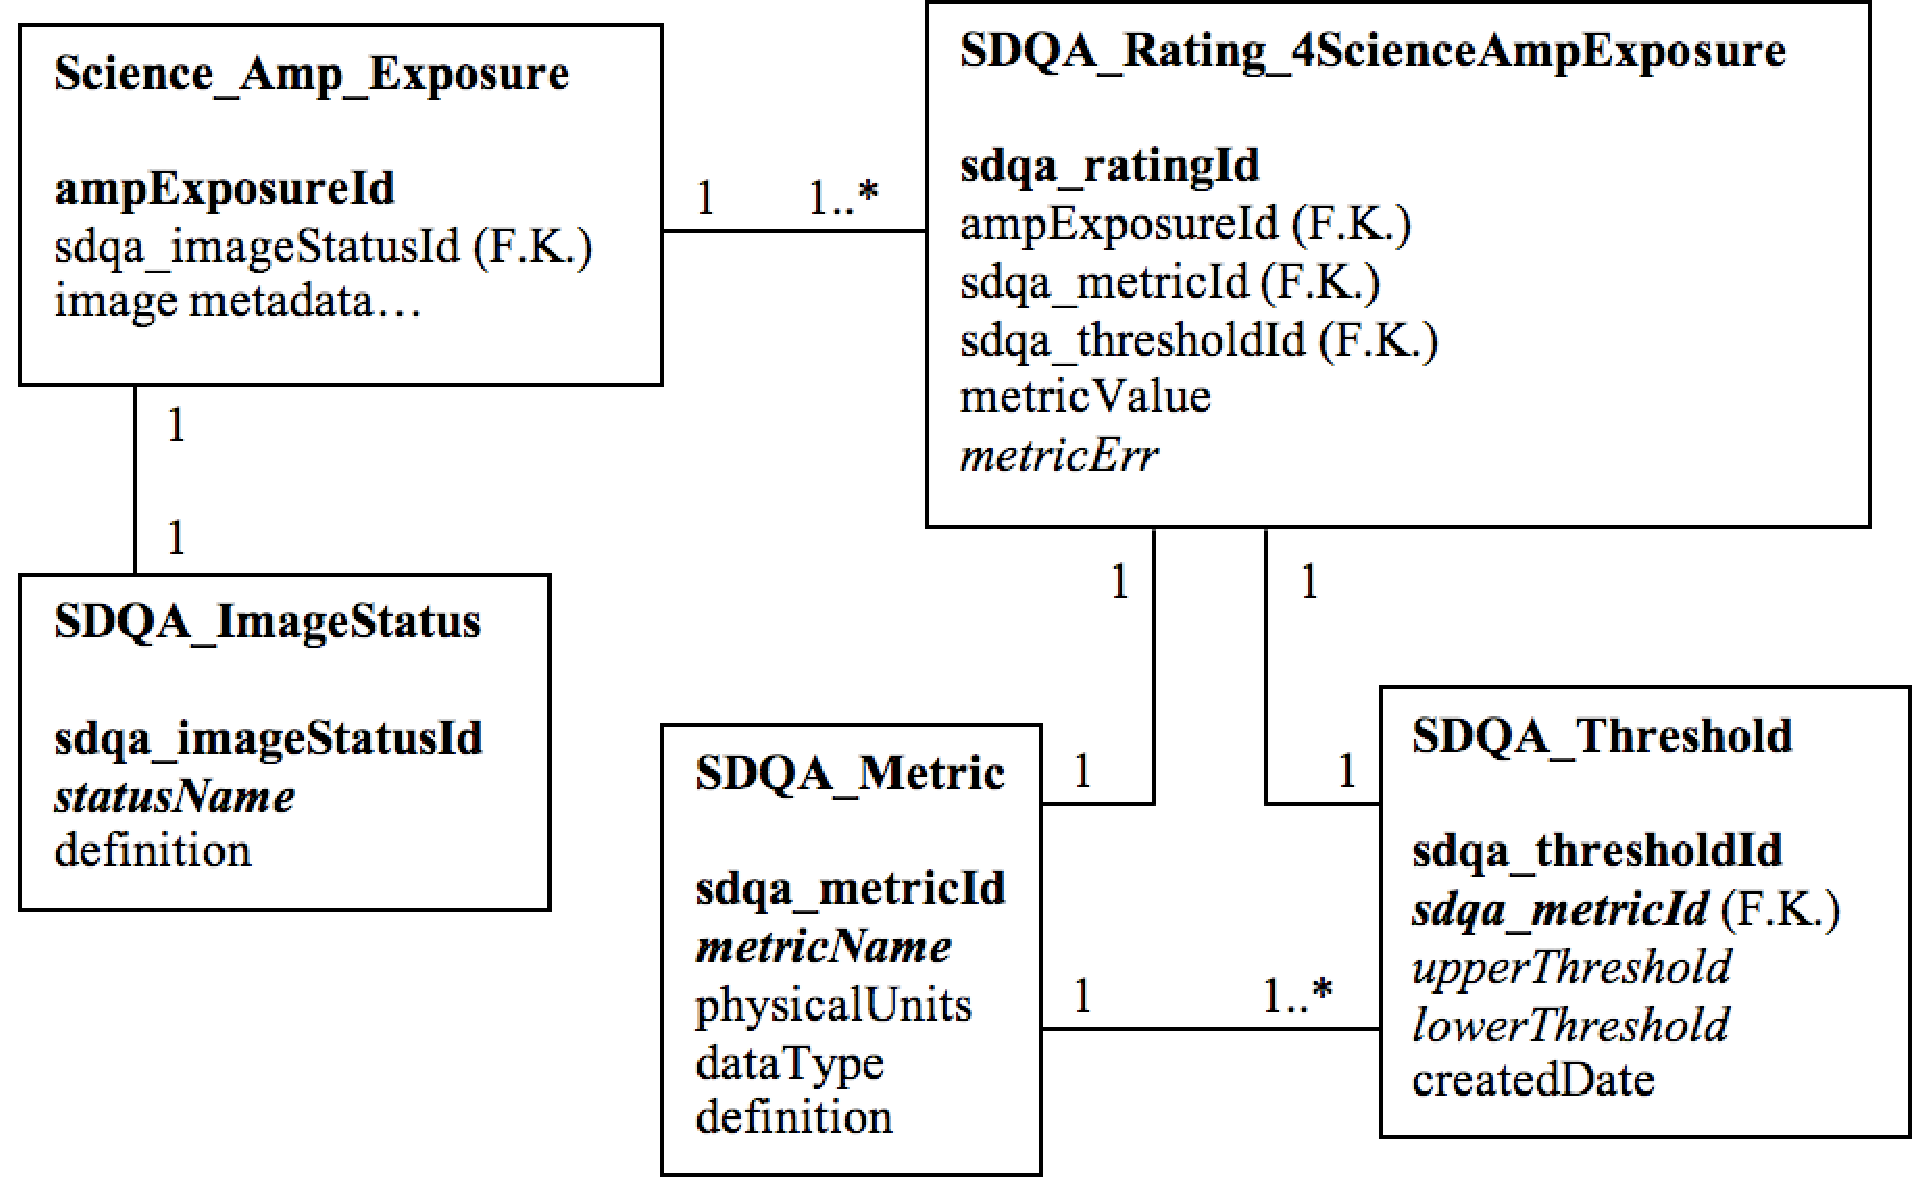
\includegraphics[scale=0.5,bb=0 0 925 573]{images/O7A2_1}
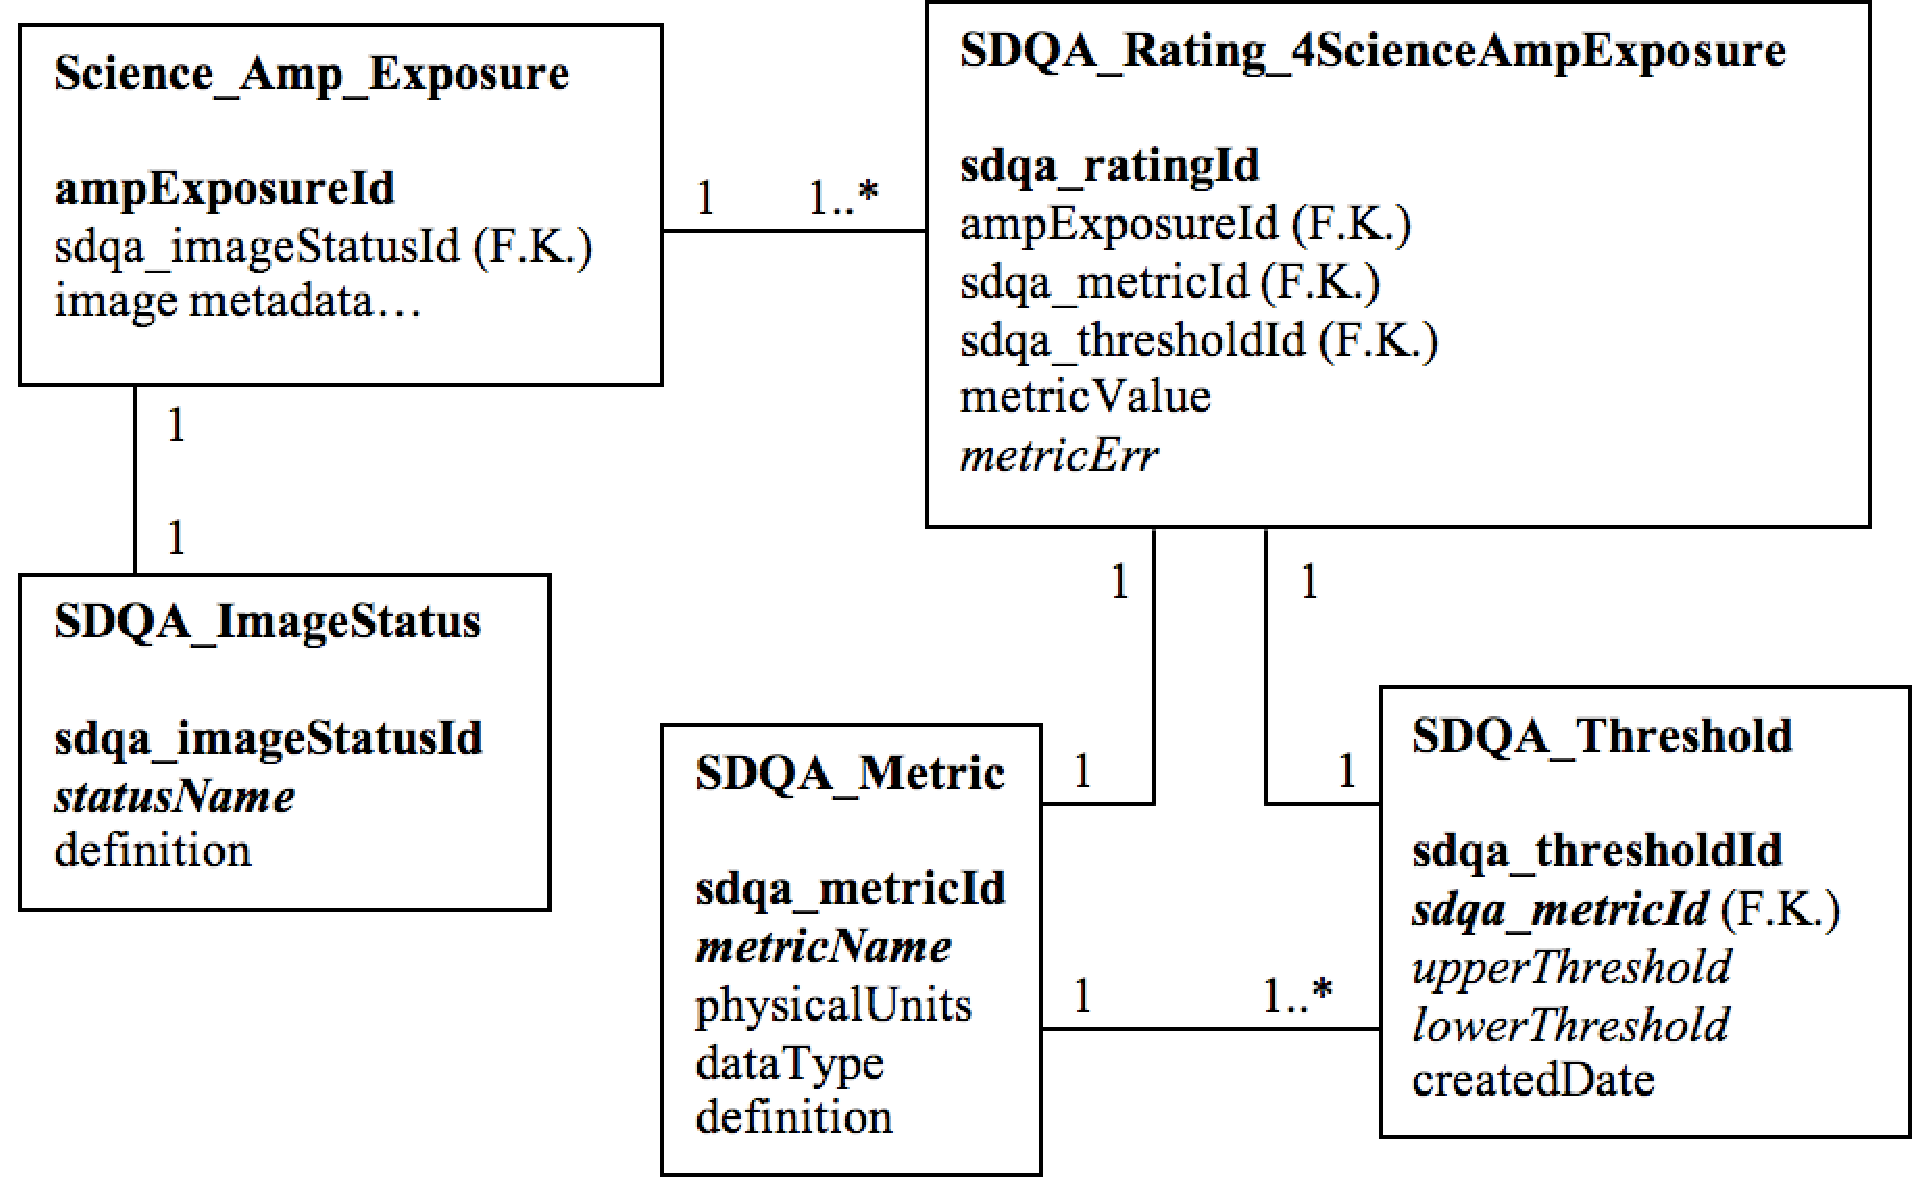
\includegraphics[scale=0.4]{images/O7A2_1}
\caption{SDQA database-schema design (``F.K.'' stands for foreign key, and ``1~{\jot 24pt}~1*..'' stands for one record to many records).} 
 \label{DB}
\end{centering}
\end{figure}

We designed and implemented a first version of the database schema for SDQA in fulfillment
of Objective \#3.  Figure~\ref{DB} shows the portion of our SDQA database-schema design
that associates SDQA Ratings with amplifier-level images.  
The primary advantage of this schema design is that persisting additional SDQA Metrics
does not require a schema change; instead you simply add new records to the SDQA\_Metric
and SDQA\_Threshold database tables to define the new SDQA Metrics and associated thresholds.
Our DC3a implementation also
includes tables for associating SDQA Ratings with image data at the CCD and FPA levels.
The schema's tables closely parallel the SDQA classes that we have identified in our UML design.

The Science\_Amp\_Exposure database table stores metadata for
processed images associated with independently read-out 
512$\times$2048-pixel portions of 
raw images (called amplifier 
segments).  The sdqa\_imageStatusId field in this table points to the grade
category determined for the image by the SDQA subsystem (although this was not populated
in DC3a, it will be done in DC3b).  
The SDQA\_Rating\_4ScienceAmpExposure database table is associated with 
the Science\_Amp\_Exposure database table in a one-to-many
relationship.  A processed image, in general, has multiple SDQA ratings, which
are computed at various pipeline stages, temporarily stored in pipeline-shared memory, and 
ultimately persisted in the database.


We accomplished Objectives \#4 and \#5 by developing and testing object-oriented C++
source code for the following classes:

\begin{itemize}
\item{SdqaMetric}
\item{SdqaRating}
\item{PersistableSdqaRatingVector}
\item{SdqaThreshold}
\item{SdqaImageStatus}
\item{SdqaRatingFormatter}
\end{itemize}

\noindent
In addition, we implemented SWIG wrappers for usage of these classes
by Python scripts directly.  We verified all SDQA-related source code
by creating unit tests and assuring their successful execution.  The
unit test for the SDQA Rating Formatter involved persisting SDQA
Ratings in a test database and then querying the database to verify
that its contents accurately match the SDQA Ratings that were
originally persisted.

All software coding was done carefully to assure that LSST coding guidelines were followed.

Although the SdqaRatingFormatter class has basic functionality for persisting SDQA Ratings
in DbStorage, it lacks capabilities for DbTsvStorage, BoostStorage, and XmlStorage.  This
will be remedied in DC3b, along with a few other inefficiencies pointed out by K.-T. Lim.

We created a package called ``sdqa'' in the LSST SVN repository and committed the SDQA-related source code there.  Release 3.0.3 of the sdqa package was used in the 
final testing for DC3a.

The next subsection demonstrates how Objective \#6 was met.


\subsubsection{Sample DC3a SDQA Ratings}

To accomplish our DC3a objective of persisting SDQA Ratings, the
image-processing pipelines were modified to instantiate SDQA-Rating
objects for various SDQA Metrics of interest in DC3a.  A tutorial was
written to give the application developers explicit instructions on
how to persist SDQA
Ratings\footnote{http://lsstdev.ncsa.uiuc.edu/trac/wiki/SdqaRatingTutorial}.
The following example illustrates how SDQA Ratings can be used to
assess the quality of the IPSD pipeline.   Below is a sampling of
ratings that were persisted to the database during a particular
production run (run ID {\tt rlp1188}):

{\tiny
\begin{verbatim}
+----------------------------+----------+---------------------+--------------------+---------------------+---------------------+
| metricName                 | count(*) | min(metricValue)    | max(metricValue)   | avg(metricValue)    | stddev(metricValue) |
+----------------------------+----------+---------------------+--------------------+---------------------+---------------------+
| ip.diffim.kernelSum        |      558 |  -0.657514177126991 |   7.98916588029419 |     4.7838537751288 |      1.420147681719 | 
| ip.diffim.residuals        |      558 | -0.0328804743717919 | 0.0019883894744249 | -0.0021186088057241 |  0.0037378047459525 | 
| ip.isr.numCosmicRayPixels  |      558 |                   0 |                  0 |                   0 |                   0 | 
| ip.isr.numSaturatedPixels  |      558 |                   0 |               2033 |      137.8853046595 |     381.85356427703 | 
| phot.psf.numAvailStars     |      279 |                   4 |                 25 |     12.992831541219 |     4.0789632806315 | 
| phot.psf.numGoodStars      |      279 |                   4 |                 25 |     12.931899641577 |     4.0955024257056 | 
| phot.psf.spatialFitChi2    |      279 |    5.02278757095337 |   1727.95910644531 |     118.54034705316 |     199.66763559788 | 
| phot.psf.spatialLowOrdFlag |      279 |                   0 |                  0 |                   0 |                   0 | 
+----------------------------+----------+---------------------+--------------------+---------------------+---------------------+
8 rows in set (0.01 sec)
\end{verbatim}
}

\noindent
This summary of the metrics was generated with the following SQL
database query:

{\small
\begin{verbatim}
select b.metricName, count(*), min(metricValue), max(metricValue),
       avg(metricValue), stddev(metricValue) 
from sdqa_Rating_ForScienceAmpExposure a, sdqa_Metric b 
where a. sdqa_metricId=b.sdqa_metricId 
group by b.metricName;
\end{verbatim}
}

For each amplifier-level image processed, SDQA Ratings for eight different SDQA Metrics 
were persisted in the database by the pipelines.  Four SDQA ratings were computed by
the PSF pipeline, two by the ISR pipeline, and two by the difference-imaging pipeline.
That different pipelines were able to persist SDQA Ratings demonstrates the flexibility of the design.

Although demonstrating the utility of specific SDQA ratings was not an
objective of DC3a (it will be an objective for DC3b), these numbers do
reveal something of the character of the processing.  Our DC3a results
analysis has suggested that extreme values of {\tt
  ip.diffim.kernelSum} are correlated with bad subtractions between
image and template, which are ultimately caused by bad astrometry.
Despite this, we do see that kernels are being generated with the
expected statistics; that is, {\tt ip.diffim.residuals} has a
near-zero mean (compared to its RMS).   The results for {\tt
  ip.isr.numCosmicRayPixels} show that no cosmic rays were detected
which may indicate a threshold-tuning issue.  Finally, our experience
has shown that there is a correlation between {\tt
  phot.psf.numGoodStars} and the positional uncertainties of
PSF-fitted source detections, and so it is expected that this will be 
a useful diagnostic.

The information in the above table represents the kind of information
that could be included in a nightly SDQA summary.  Since the SDQA
ratings are stored in the database, it is easy to construct a variety
of useful queries; e.g., all {\tt phot.psf.numAvailStars} values for a
given night, CCD, and filter.

Although SDQA Thresholds were not tuned for DC3a, we expect this to be
a component of the work for DC3b.


\subsubsection{Advanced Assessment Techniques}

In our ADASS paper (Laher {\it et al.}~2008), we pointed out that the method of 
artificial neural networks is particularly promising for classifying images in 
terms of SDQA (see Figure~\ref{ANN}).  In late 2008 we undertook some work 
involving ANNs to demonstrate that various attributes of extracted
source detections could be used to differentiate between variable QSOs
and non-variable white dwarfs \citet{borne09}.  Our completeness and
reliability results showed that ANNs  are superior to the method of
segmenting the two populations in conventional color-color plots\footnote{
http://spider.ipac.caltech.edu/staff/laher/lsst/borne\_696\_Jan09-ver2.pdf
}.

\begin{figure}[htb]
\begin{centering}
% \epsscale{0.2}
% \plotone{images/O7A2_2}
%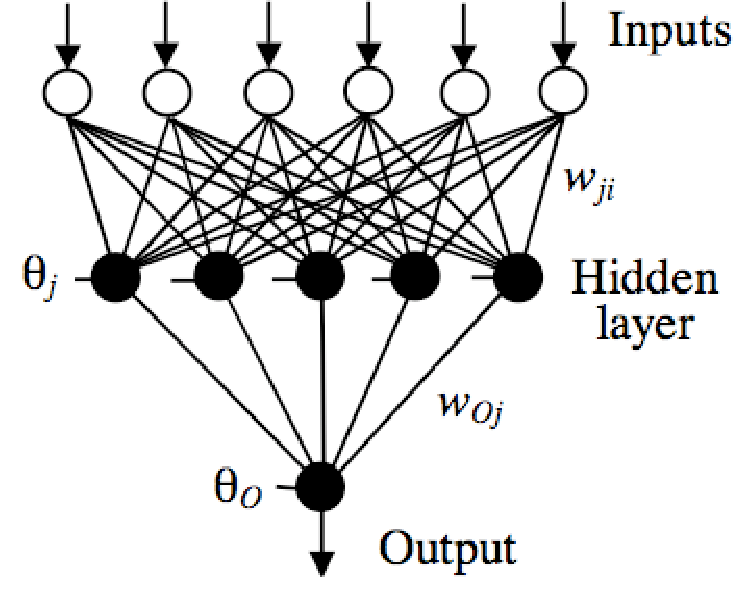
\includegraphics[scale=0.5,bb=0 0 363 285]{images/O7A2_2}
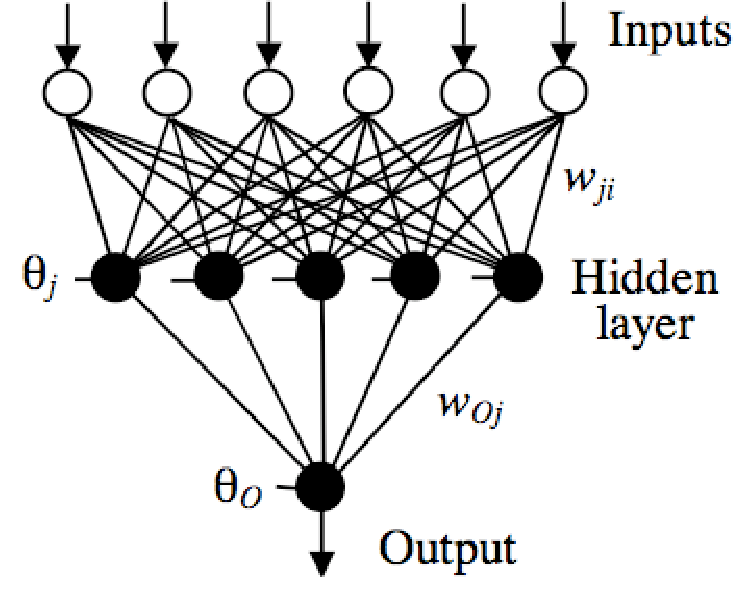
\includegraphics[width=3in]{images/O7A2_2}
\caption{Artificial neural network with single-hidden-layer architecture.} 
 \label{ANN}
\end{centering}
\end{figure}


One of IPAC's current projects is development of image-processing pipelines and data archive
for the Palomar Transient Factory (PTF), a new 12-CCD camera recently installed on the Palomar
48'' Schmidt Telescope.  This camera is now in operations and acquires up to $\approx 4,800$
CCD images per night (2K$\times$4K pixels per CCD), 
which are subsequently sent to IPAC for processing and archiving.  
While this project is separately funded, we have been able to use
it fruitfully as a test bed for prototyping LSST-SDQA-subsystem designs.  
To be clear, the utility of PTF for our LSST purposes are:

\begin{enumerate} 
\item{Validating our choices for metrics that may be useful for LSST (since PTF is a 
time-domain project with some overlapping science goals).}
\item{Technology exploration.}
\item{Exploring visualization strategies for representing very complex and 
voluminous SDQA data in a comprehendible way.}
\end{enumerate} 

We have
implemented for PTF a fully automated SDQA subsystem of the design essentially
envisioned for LSST.  The PTF image-processing pipeline now populates more than 40 different
SDQA metrics in the PTF database.  A process for thresholding SDQA ratings and determining 
SDQA statuses for processed images has been implemented as a database stored function and
integrated into the PTF image-processing pipeline.  An indispensible software tool developed 
as a result of this effort is a web-browser-based SDQA GUI, which facilitates viewing of raw and
processed images and time-series plots of SDQA ratings over a specified observing night 
(see Figures~\ref{PTFSDQAGUI1} and~\ref{PTFSDQAGUI2}).  Much of the source 
code for the PTF SDQA GUI was leveraged from Java classes developed over the last ten years at 
the Spitzer Science Center (SSC) for observation planning, image visualization, and the
Spitzer Heritage Archive interface.  The PTF SDQA GUI is a Google Web Toolkit application that
queries the PTF database for image metadata and SDQA data to display and plot.  One of our
objectives for LSST in DC3b is to further develop the SDQA GUI for LSST use, i.e., set it up to 
query and visualize LSST databases and image archives.

\begin{figure}[htbp]
\begin{centering}
% \epsscale{1.0}
% \plotone{images/PTFSDQSGUI1}
%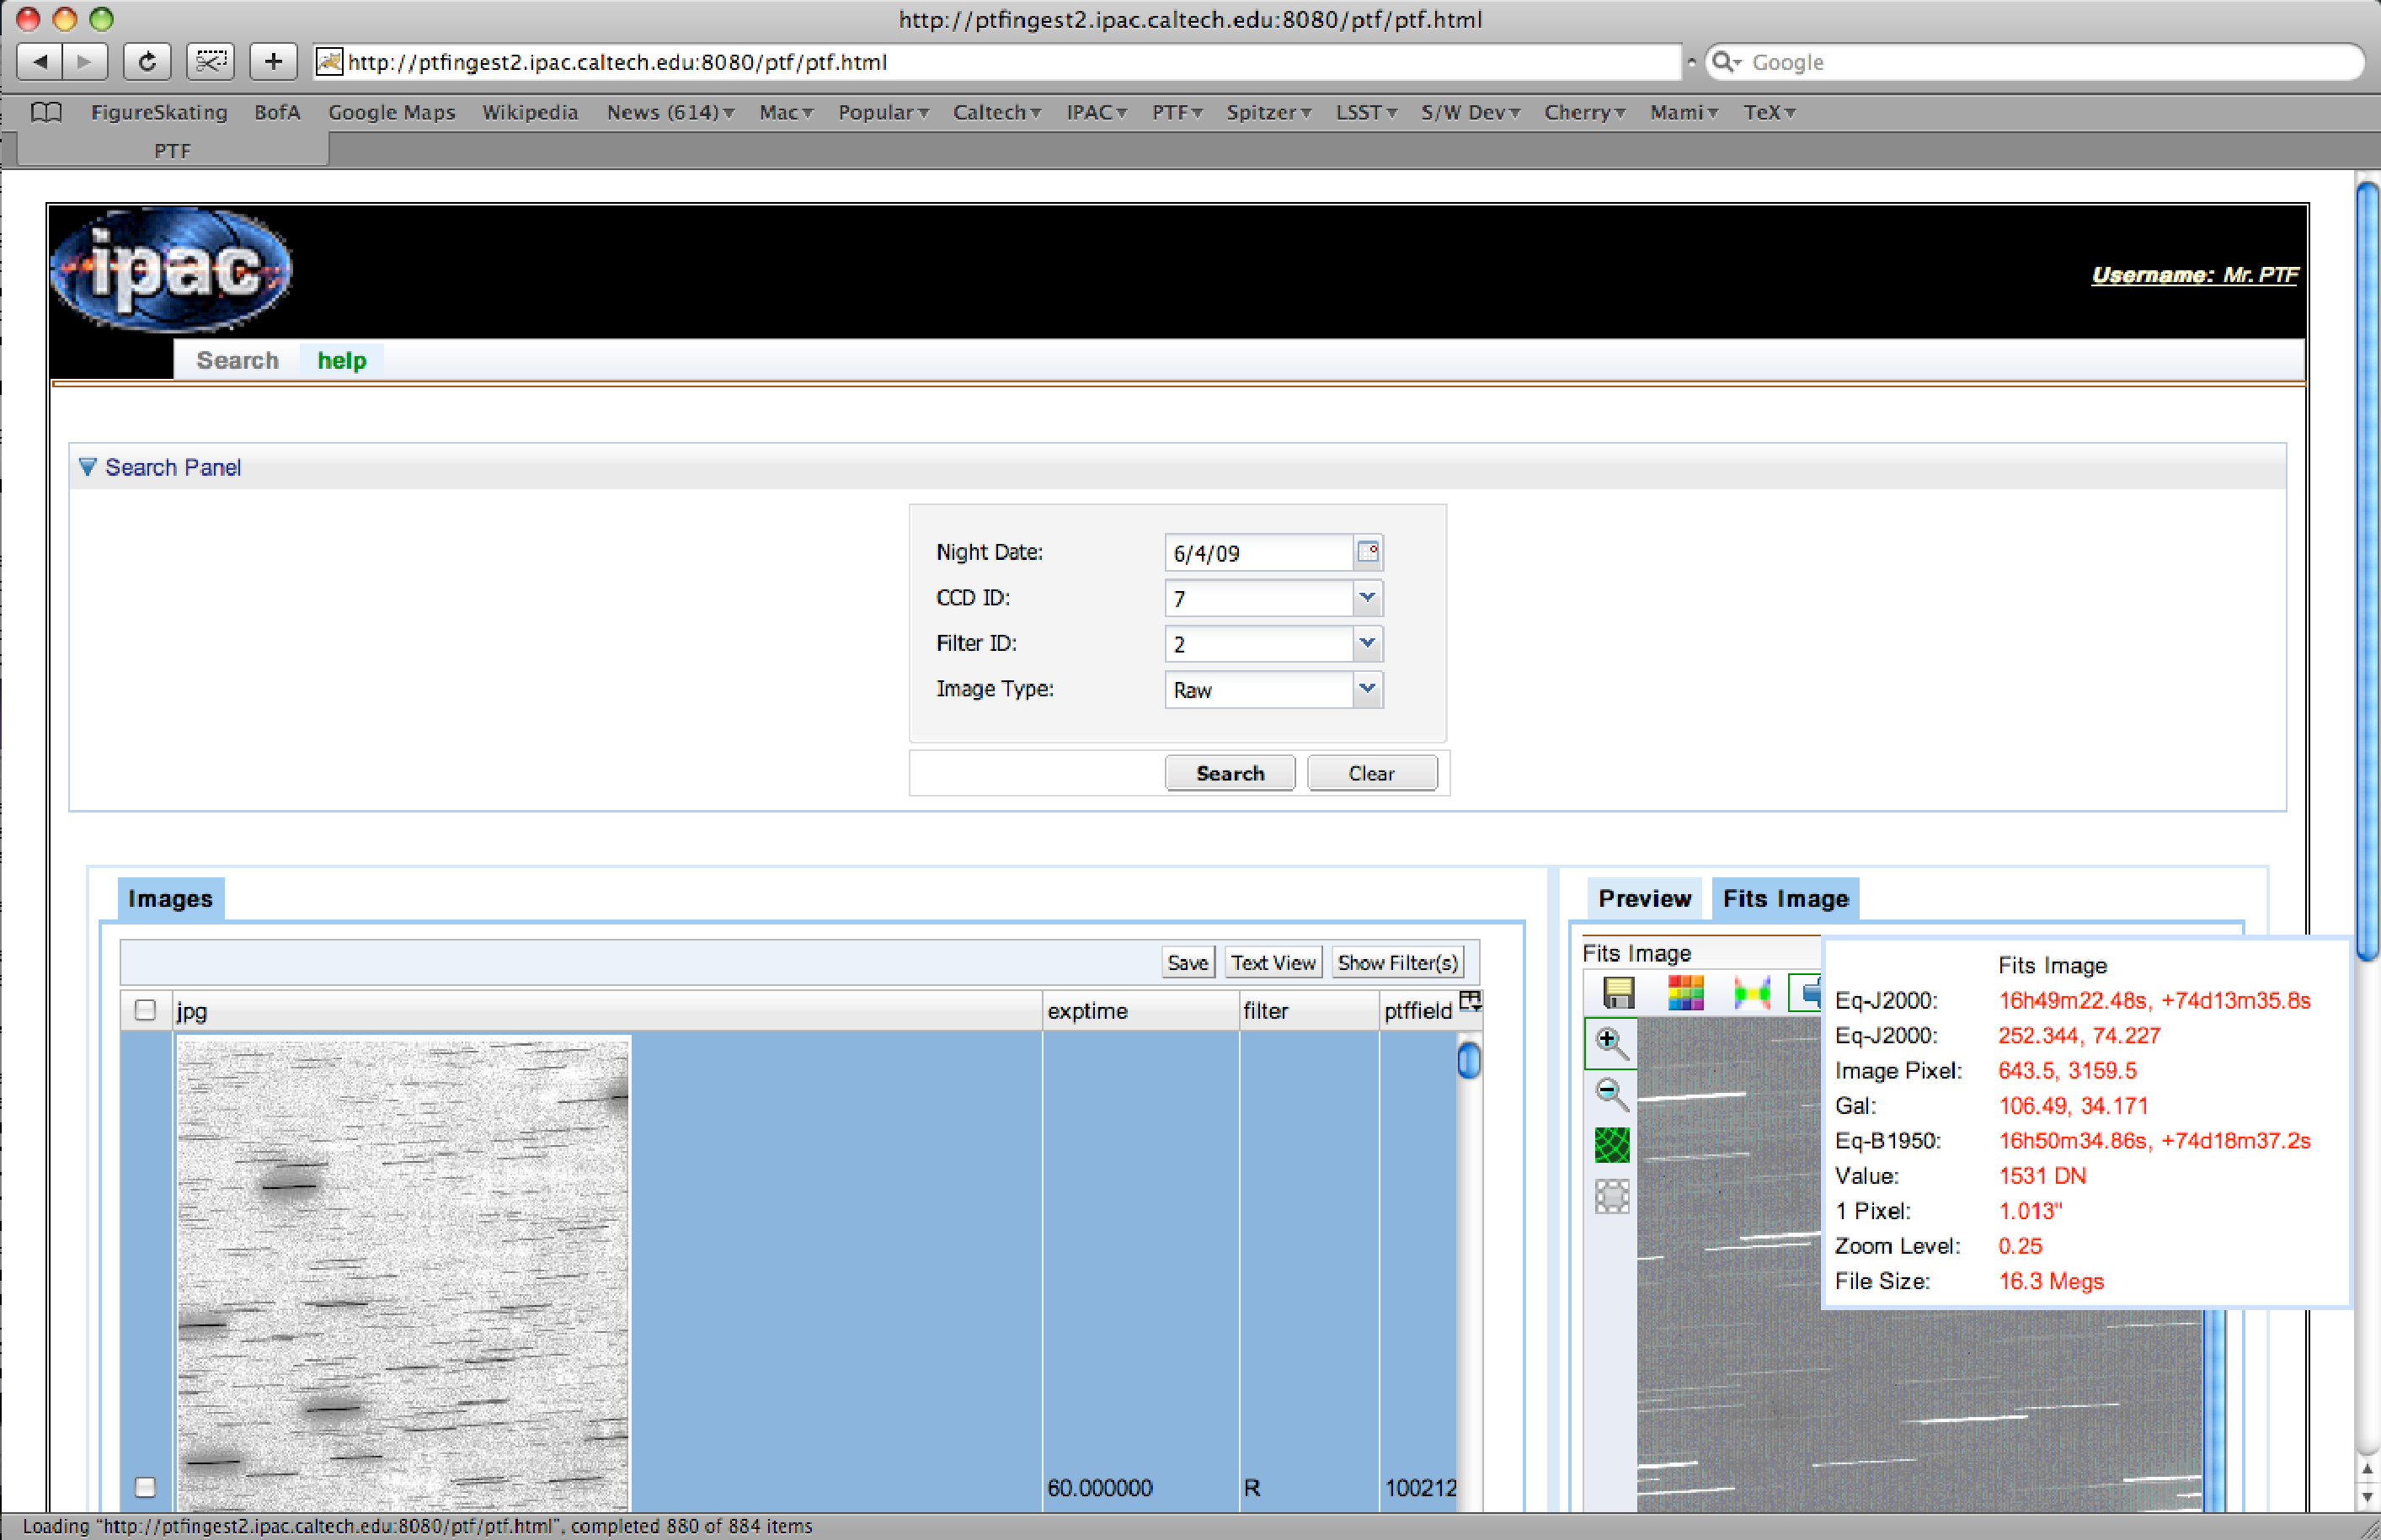
\includegraphics[width=\textwidth,scale=0.5,bb=0 0 1357 878,clip]{images/PTFSDQSGUI1}
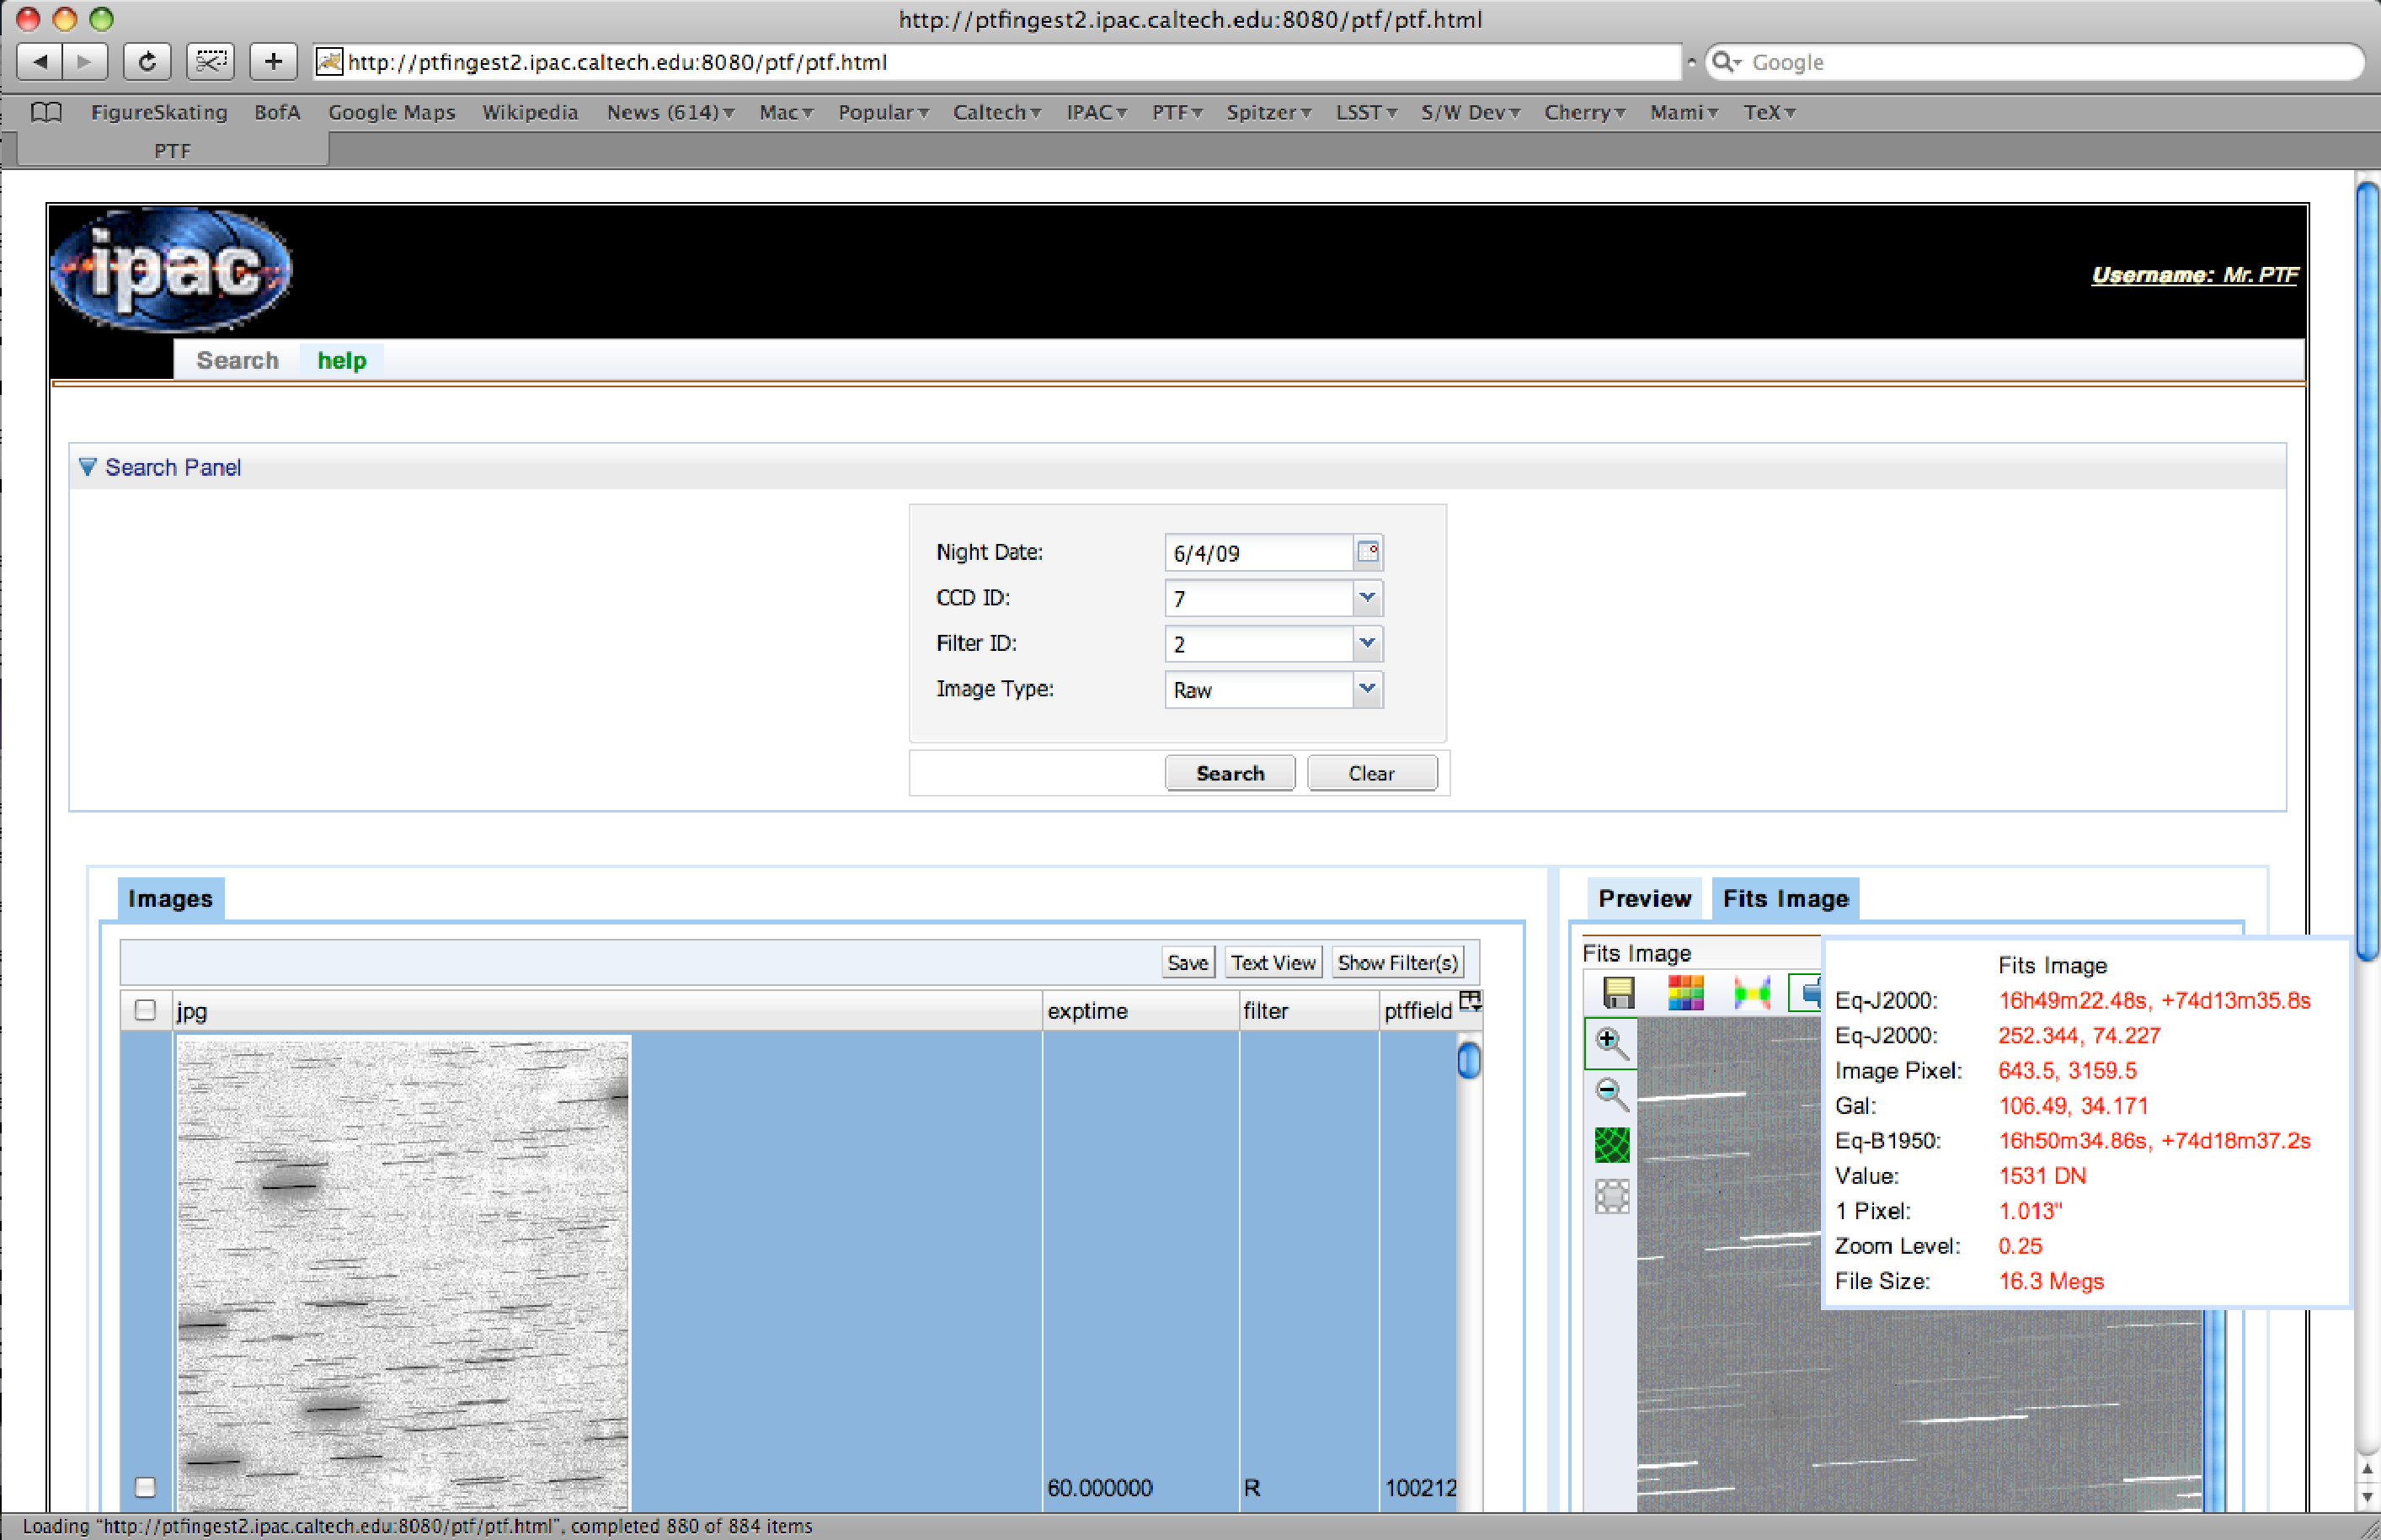
\includegraphics[width=5in]{images/PTFSDQSGUI1}
\caption{PTF SDQA GUI screen shot showing image display from query of PTF database.} 
 \label{PTFSDQAGUI1}
\end{centering}
\end{figure}

\begin{figure}[htbp]
\begin{centering}
%\epsscale{1.0}
%\plotone{images/PTFSDQSGUI2}
%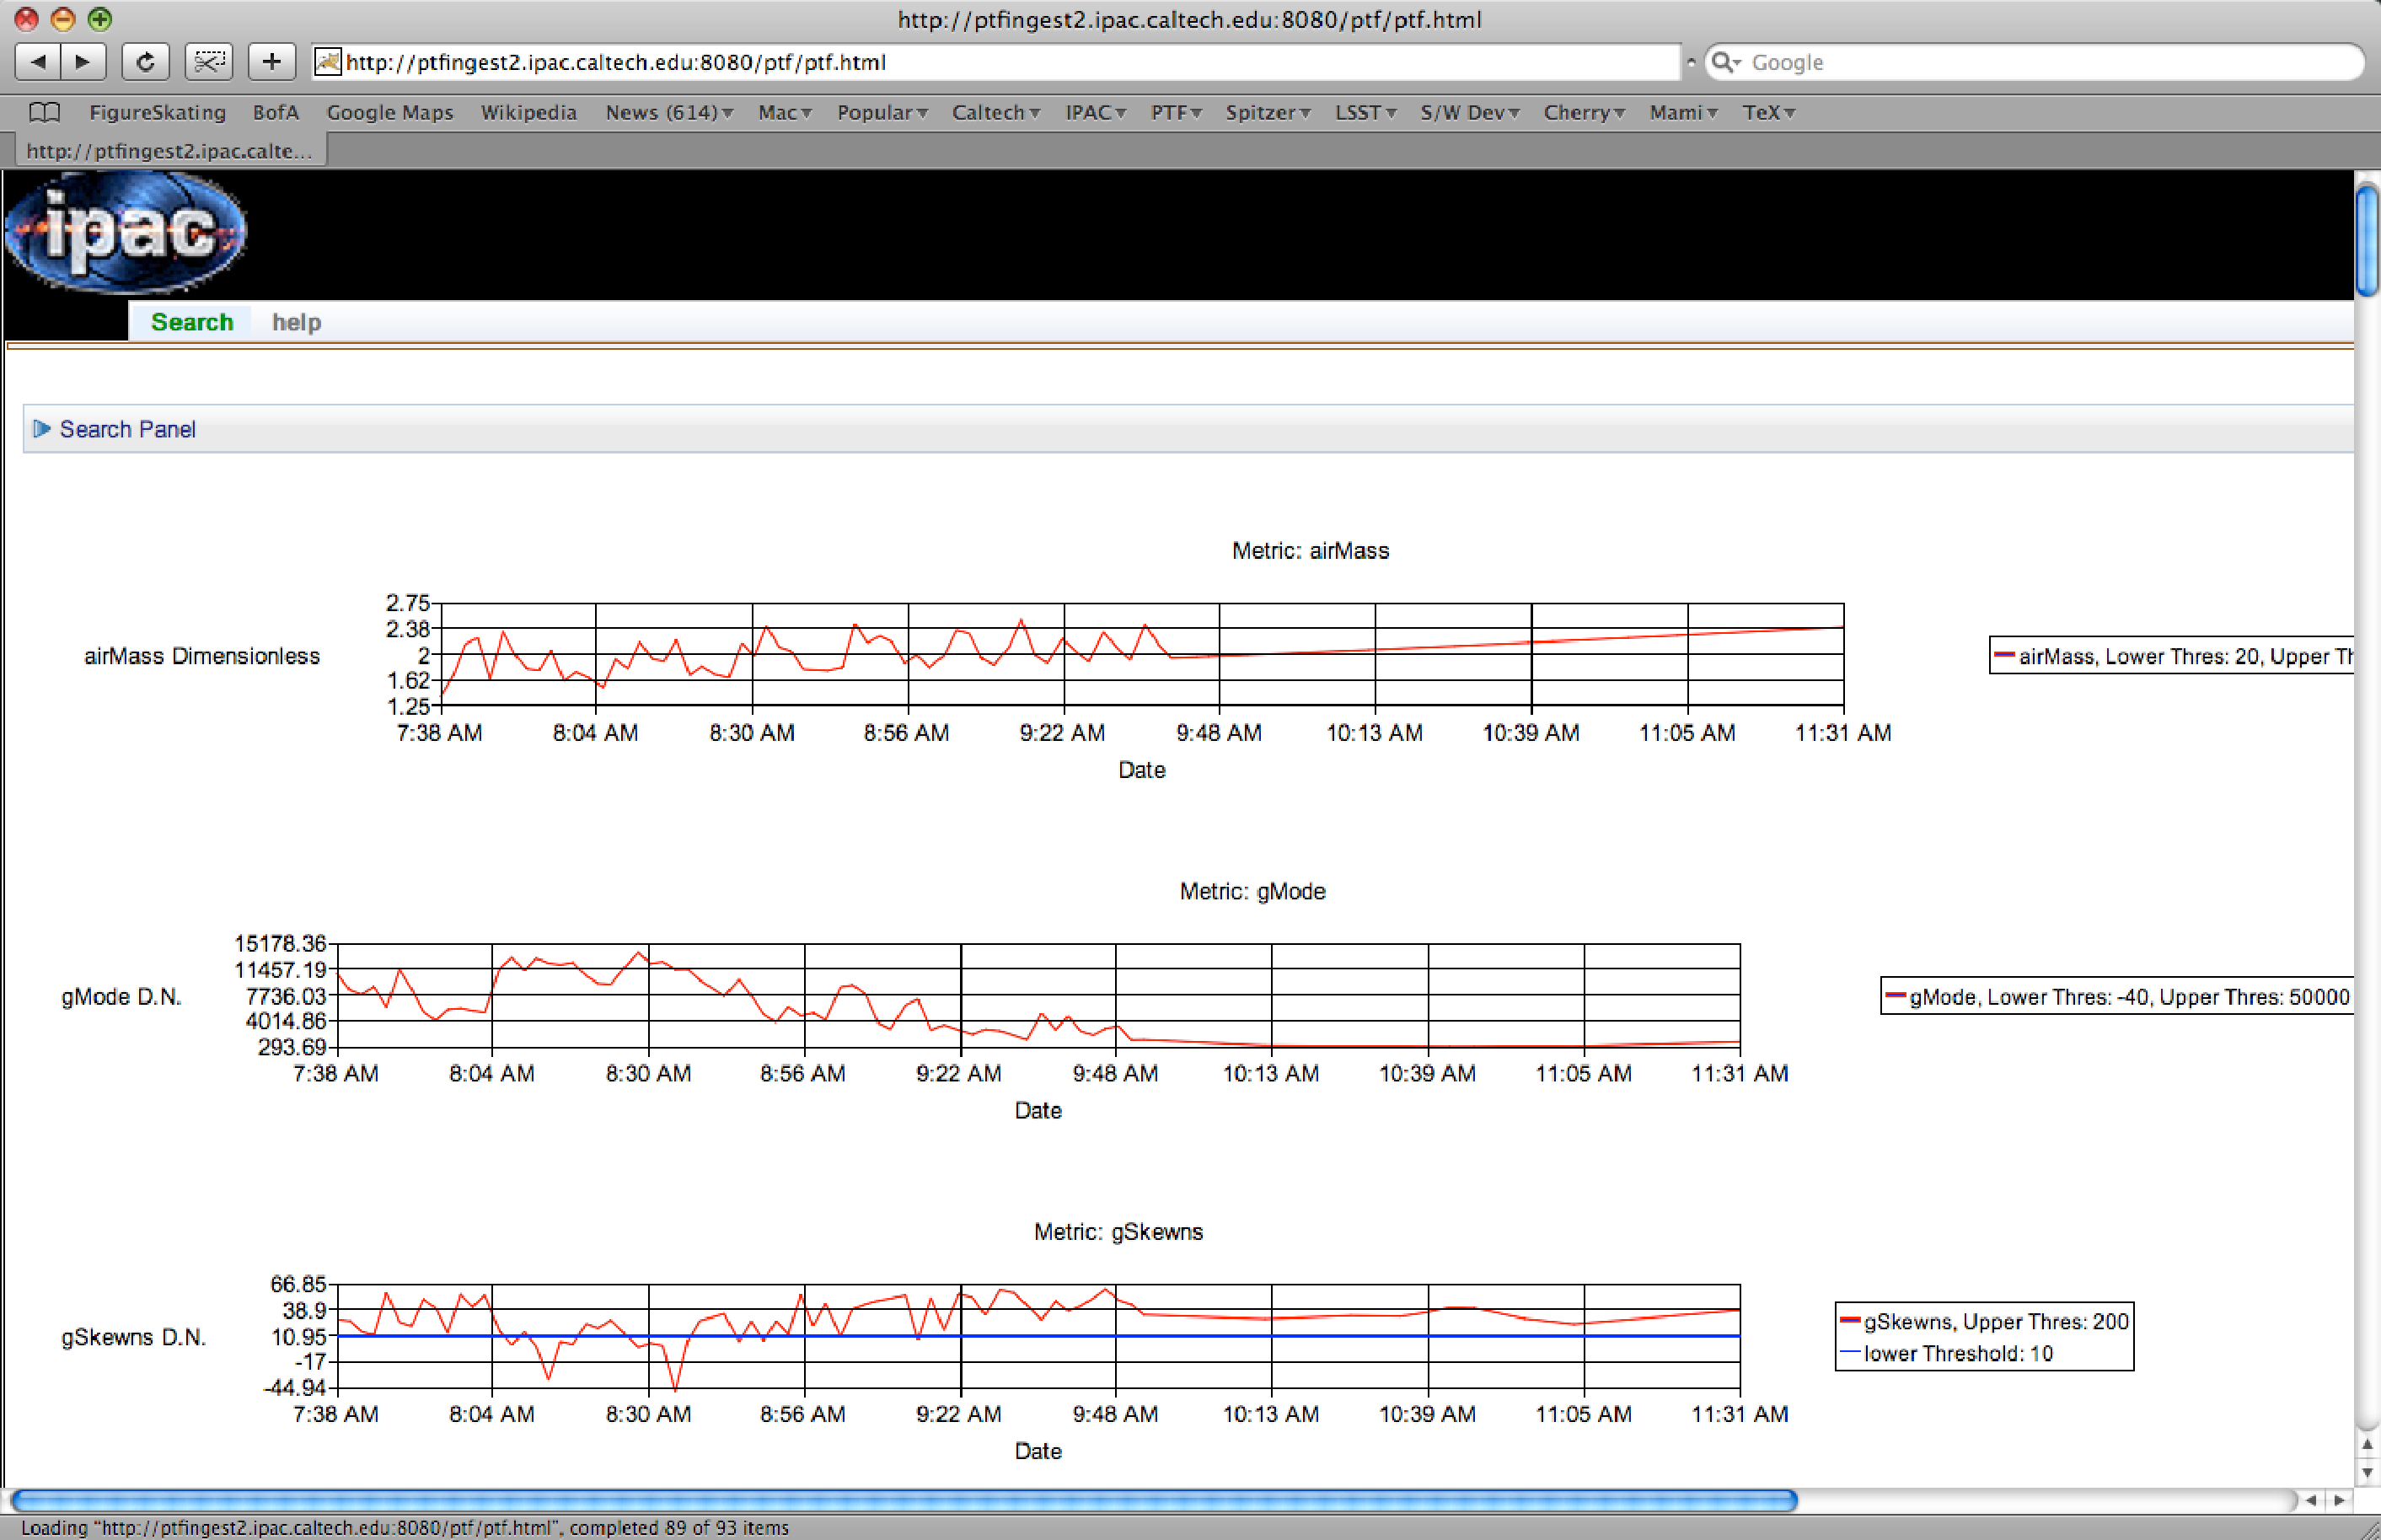
\includegraphics[width=\textwidth,bb=0 0 1356 877,clip]{images/PTFSDQSGUI2}
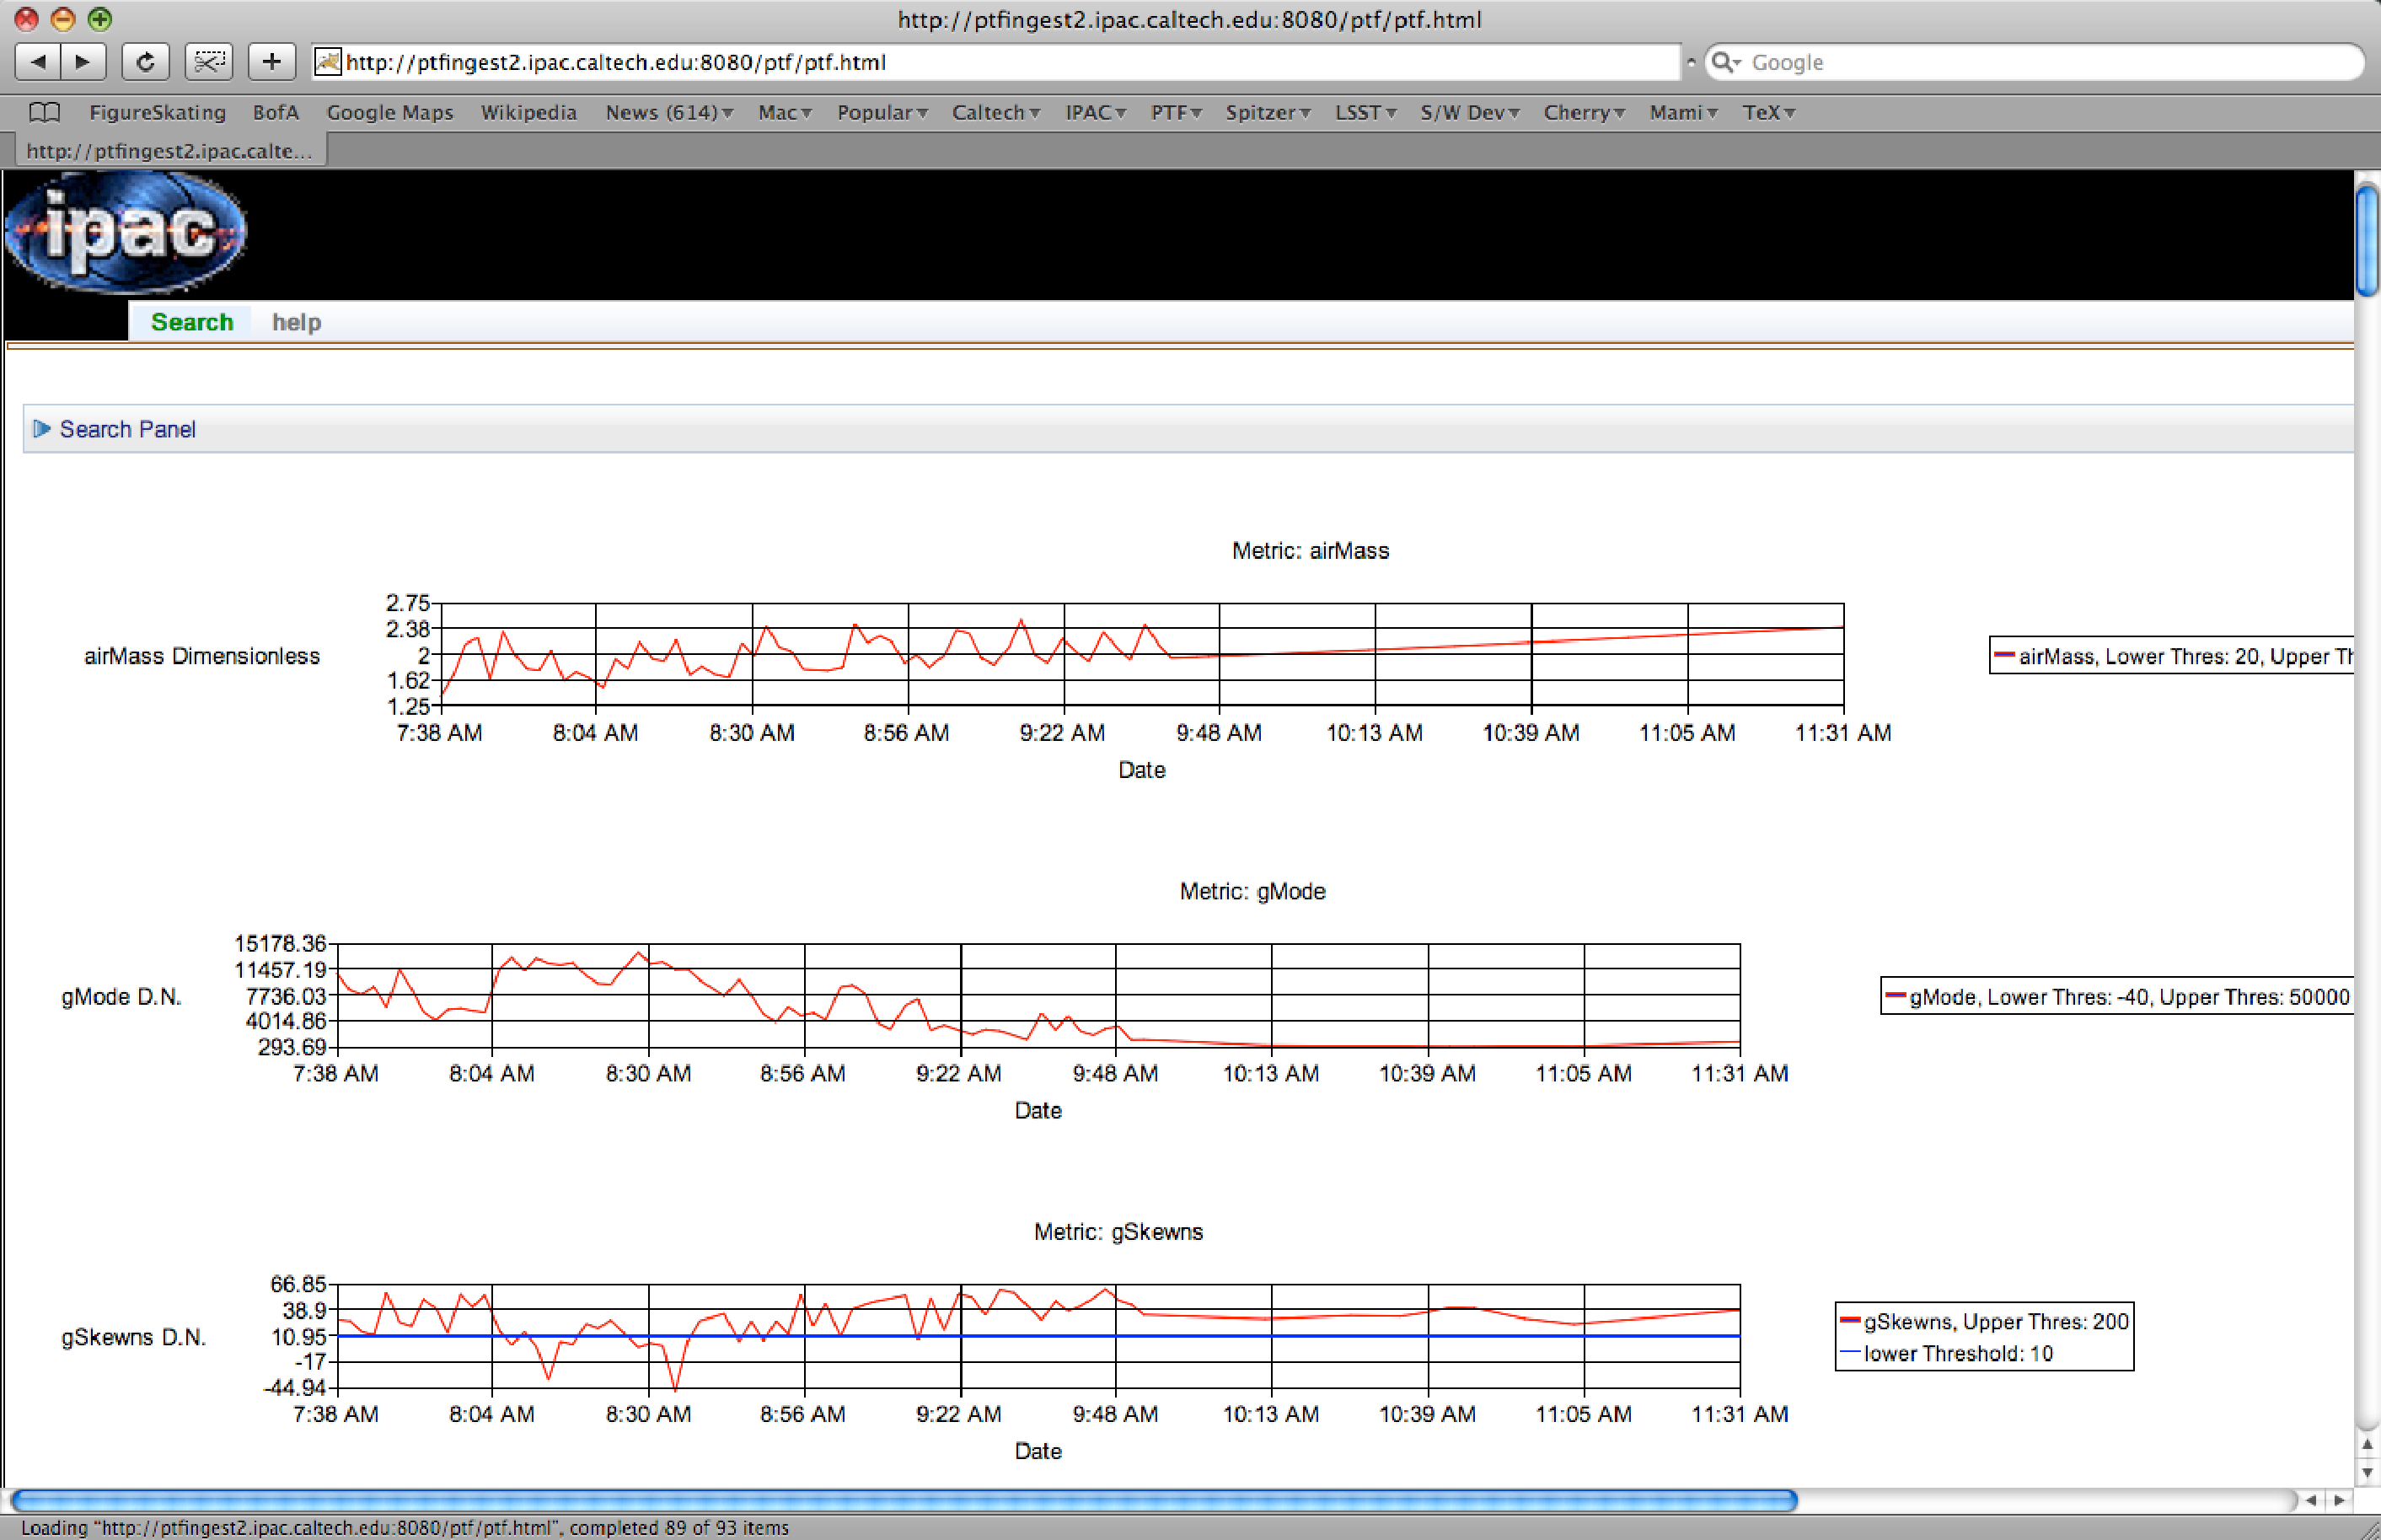
\includegraphics[width=5in]{images/PTFSDQSGUI2}
\caption{PTF SDQA GUI screen shot showing SDQA time-series plots from query of PTF database.} 
 \label{PTFSDQAGUI2}
\end{centering}
\end{figure}


% -- Section 7
% Section 7: Results

\section{Results}

\subsection{Summary of Runs}

Much as with DC2, we executed numerous but short pipeline runs over
a sampling of the data from the CFHT-LS fields D3 and D4 and from the
simulated data collections, SimDeep and SimWide.  These short runs
were used to do initial debugging, performance analysis, and quality
analysis which resulted in numerous bug fixes and important algorithm
optimizations.  These short runs also allowed to explore different
policy parameter settings to understand the trade off between data
quality and performance.  

For our final, detailed analysis of the data quality and processing
performance, we focused on two productions runs with identical
versions of the software and configuration: {\tt rlp1233} and {\tt
rlp1234}.  As summarized in Table \ref{T7-1}.  These two runs
processed different subsets of the focal plane for 85 visits to the
CFHT-LS D3 on our own LSST cluster.  These visit were selected based
on the availability of the calibration data needed to calibrate raw
science images.  The Image Processing and Source Detection (IPSD)
pipeline featured 1 master pipeline and 31 slice processes running
across four nodes of the cluster (thus each run processed 31 amplifier
images in parallel).  The Association pipeline (ap) ran on node 10
within one master process and one slice process.  The ``NightMOPS''
pipeline (part of the Moving Objects Prediction System) ran on node 9
with 1 master process and 5 slice processes.  Taking a lesson from
DC2, we did not use any of the ``slower'' cluster nodes (nodes 1-4)
for pipeline processes as they would have pulled down the over
performance of the pipeline.  We note that we had other infrastructure
processes on the cluster nodes running which did not interfere
noticeably with the pipeline processes.  Node 4 (which did not have
any pipeline processes on it) hosted the event broker process, and
node 9 (which had extra unused processor cores available) hosted the
event monitor which loaded logging events into the database.

One of the intended goals of the DC3a was exercise the use of the
parallel filesystem, Lustre, we installed on the LSST cluster.  Much
as with DC2, we found Lustre to be fairly unstable under heavy IO,
apparently causing catastrophic failure of the filesystem.  This may
have been due to an insufficient number of fileserver nodes for the
level of IO we were attempting; however, schedule and hardware
resource limitations prevented our exploring the causes in any
detail.  Consequently, the final runs were conducted using NFS-mounted
filesystems (which are known to perform poorly under most conditions).  

Ultimately, the simulated data was not used as part of the final
analysis.  While the two simulated collections were instrumental
in understanding and correcting processing problems, we found that the
quality of the template images were insufficient for producing useful
difference images and database results.  

In addition to the runs on our own LSST cluster, we also conducted
runs on the NCSA Abe cluster.  The purpose of these runs were to
explore the scalability of the pipeline processing up to higher
numbers of slices.  In particular, we have executed runs that process
entire CFHT focal plane exposures simultaneously.  This was done by
running the IPSD pipeline on Abe with 288 slice processes across 36
8-core nodes.  While Image I/O was carried out using the Lustre
filesystem attached to that platform, database I/O occurred with the
database residing on the LSST cluster ({\tt lsst10}).  

DC3a schedule constraints limited the detailed analysis
that could be completed for this report; nevertheless, we see that the
pipeline scaled fairly well at this level.  One critical barrier to
scaling, however, was in the event broker (powered by the
third-party product, activemq), which failed while processing the
thirteenth visit which in turn disabled the pipelines.  The reasons
are unclear; though, it appears to be due to the total volume of
events processed rather than the rate of at which the events were
generated.  

These Abe runs provided additional qualitative accomplishments:

\begin{itemize}
\item they revealed configurable system limits that must be increased:
\begin{itemize}
\item the event broker must support over 1000 simultaneous open file
  descriptors 
\item the MySQL database must support $\gtrsim$ 300 simultaneous
  connections.  
\end{itemize}
\item we demonstrated the integration of grid-based job management
  (via Condor-g) into our orchestration layer
\item we demonstrated the successful use of the parallel Lustre
  filesystem.  
\end{itemize}

\noindent Additional information about the results of these runs on
Abe can be found in section \ref{sec:timing}.  

Table \ref{tbl:runsummary} summarizes the pertinent production runs
referenced in this section.

\begin{table}[hp]
\centering
\caption{Summary of Production Runs analyzed in this report
\label{tbl:runsummary}}
\vspace{\baselineskip}
\begin{tabular}{rccccc}
\hline\hline
          &         &       & \multicolumn{3}{c}{Images Processed: Num/Size} \\
runId     & nVisits & nAmps & Raw Images & Ancil. Images & Output Images \\ \hline
rlp1233   & 85      & 31  & 5146/24 GB    & 88/13 GB       & 60525/240 GB \\ 
rlp1234   & 85      & 31  & 5146/24 GB    & 88/13 GB       & 60525/240 GB \\ 
rlpabe041 & 12      & 288 & 3456/33 GB    & 15/2 GB        & 79368/313 GB \\ \hline
Total     & ---     & 250 & 13748/81 GB   & 191/28 GB      & 200418/793 GB \\ \hline
\end{tabular}
\end{table}


\subsection{Science Data Quality}
We chose several areas for which to assess the scientific data quality of the DC3a outputs:
\begin{itemize}
\item Cosmic ray rejection
\item WCS accuracy
\item Difference image quality
\item Difference image lightcurve quality
\item Recovery of known solar system objects
\end{itemize}
Other areas could of course be added to this list, but the ones chosen
are judged to be the most demanding for the software system to meet,
and are each directly related to science requirements. 
\paragraph{Cosmic Ray Rejection}
The DC3a processing flow contains two methods of rejecting cosmic
rays, that can be used as alternatives or in tandem.  For the DC3a
reference runs, the two methods were used in tandem.
\begin{itemize}
\item As presented in section \ref{sec:isr}, the ISR detects and
  interpolates over cosmic rays in individual images
\item The Association Pipeline (AP) makes use of the two exposures per
  visit organization of the survey to discriminate against cosmic
  rays.  A positive flux DIASource present in only a single exposure
  of a visit will be considered a cosmic ray.
\end{itemize}
Quantitative analysis of the ISR cosmic ray rejection analysis method
has been performed by comparing the number of pixels affected by
synthetic cosmic rays in the e1 visit with the number identified as
cosmic rays by the ISR.  The fraction successfully identified is
nearly 100\% for rlp1233.  Analysis of the performance of the AP based
method has proven to be difficult when run in tandem with the ISR
method, and will require a separate set of runs with the ISR method
turned off.  The joint analyis will lead to an optimized cosmic ray
rejection technique for DC3b.
\paragraph{WCS Accuracy}
The WCS determination algorithm is implemented as part of the Image
Characterization Pipeline (ICP), and is discussed in section \ref{sec:wcs}.
The achieved WCS accuracy is crucial for subsequent processing,
especially for production of difference images.  The procedure used to
assess the WCS accuracy is as follows:
\begin{itemize}

\item A set of exposures from visits processed by a particular run is
  picked for analysis. For each exposure:
\begin{enumerate}
\item The WCS\_Sources identified by the ICP for WCS determination are retrieved from the
  science database for the run.
\item The pixel coordinates for each WCS\_Source are converted from
  ccd coordinates to amplifier coordinates, and are input to the
  wcstools program ``xy2sky'' along with the corresponding amplifier
  science image to yield predicted sky coordinates for the
  WCS\_Source.
\item The star catalog used for WCS determination is searched for the
  predicted sky coordinates.  The distance between the predicted sky
  position and the nearest catalog object is recorded in an output file
\end{enumerate}
\item A histogram of the distances is calculated, and its properties
  used as metrics for WCS performance.
\end{itemize}

Figure \ref{fig:wcs1} shows the resulting histograms for typical
exposures from runs rlp1233 (visit 695833-e0) and rlp1234 (visit
696554-e0). Both histograms show very similar behavior, with the peak
of the histogram around 30 mas, about 0.2 pixel.  In both cases there
is a shallow tail that extends to large distances, beyond the plotting
limit in the figure.  Figure \ref{fig:wcs2} shows that the tail is
far more significant than is initially apparent, since it
results from very poor wcs fits that are confined to individual
amplifiers.

For DC3a purposes, we define WCS failure for an image to occur when
more than 50\% of the predicted WCS\_Source positions are in error by
more than 1 arcsec.  This is roughly the level beyond which the difference
image matching kernels can no longer compensate for image misalignments. With
this criterion, for run rlp1233 there were 109 failures out of 2629
images processeed, or 4\%.   For rlp1234 there were 14 failures out
of 2509 images processed, or 0.5\%.  It must be noted however, that this criterion for WCS failure will
need to be considerably stricter for DC3b and beyond, because
processing of image stacks for deep detection and measurement, and the
determination of astrometric models all require much better WCS quality.
\begin{figure}[htb]
\begin{center}
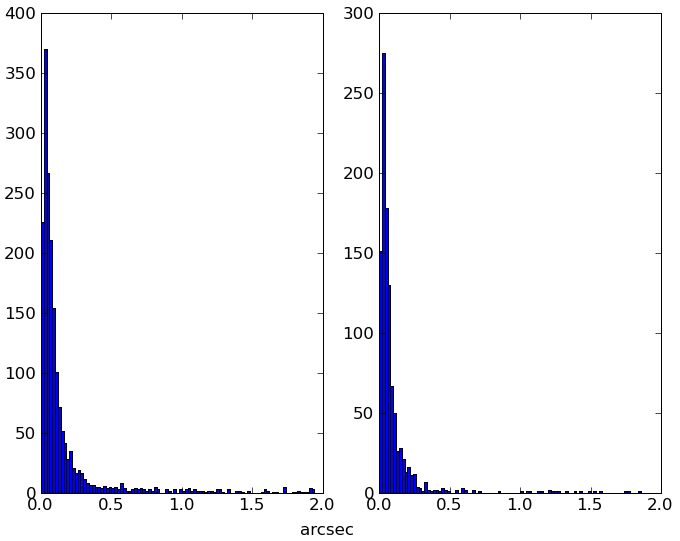
\includegraphics[width=6in]{images/rlp1233_1234_match.png}
\caption{Histogram of the distances between positions predicted from WCS, and
  true catalog positions for rlp1233/695833-e0 on the left and
  rlp1234/696554-e0 on the right}  
\label{fig:wcs1}
\end{center}
\end{figure}

\begin{figure}[htb]
\begin{center}
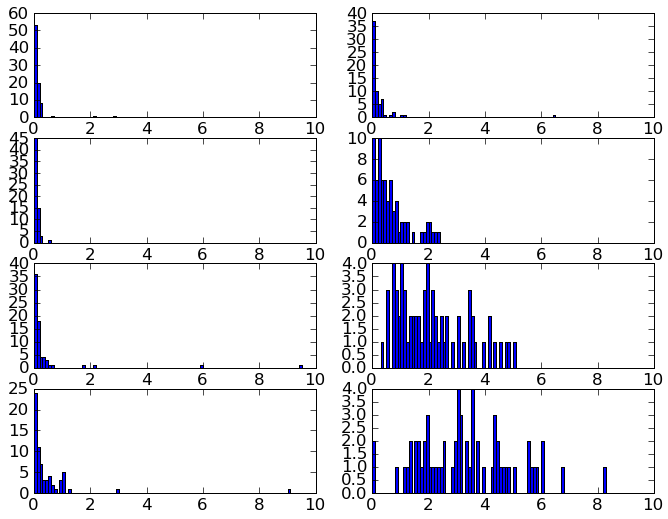
\includegraphics[width=6in]{images/rlp1233_ccd1_match.png}
\caption{Histogram of the distances between positions predicted from WCS, and
  true catalog positions for rlp1233/695833-e0, showing the individual
amplifiers from ccd1}  
\label{fig:wcs2}
\end{center}
\end{figure}



\paragraph{Difference Image Quality}

Visual inspection of DC3a difference images shows three distinct
categories. First, difference images produced from images with failed 
WCS's show either ``bipolar'' subtractions in the case of failures
near the cutoff criterion, or completely nonfunctional subtractions in
the case of extreme WCS failures.  Images with successful WCS's
generate subtractions that look good except in the vicinity of bright
stars,where a high spatial frequency pattern is evident.  Examples of
these three categories are shown in Figure \ref{fig:diffim1}.

In the remainder of this discussion, we leave aside the roughly 2\% of
the difference images that involved WCS failures, since they tell us
little about the performance of the difference image algorithm itself.
In the absence of variable or moving sources, an ideal difference
image will have a mean of zero, and show uncorrelated random
fluctuations at the level expected from the variance of the input
images.  We therefore define a ``figure of merit image'' as
\begin{equation}
f(x,y)~=~d(x,y)/\sqrt {v(x,y)}
\end{equation} 

where $f$ is the figure of merit, $d$ is the difference image, and $v$
is the predicted variance image.  A typical figure of merit image is
shown in Figure \ref{fig:diffim2}.  A plot along a horizontal line through
the subtracted bright star near the center of the image is shown in
Figure \ref{fig:diffim3}.  This plot shows several aspects of the difference
image quality:

\begin{itemize}
\item The average level of the image is near zero, as expected
\item Away from bright stars, the level of the noise is near 1.0, the
  expected value
\item In the footprint of bright stars, the noise is larger than
  expected by a large factor, about 20 in this particular case.
\end{itemize}  

\begin{figure}[htb]
\begin{center}
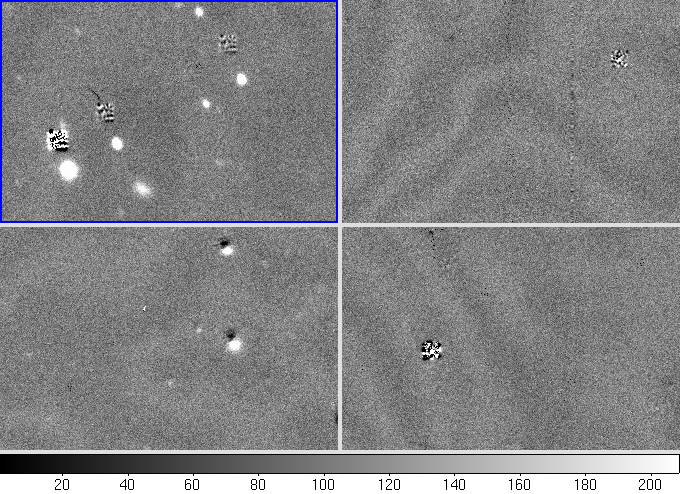
\includegraphics[width=6in]{images/rlp1233_v695833-e0-c001-mosaic.png}
\caption{A mosaic of different types of difference images, all from rlp1233/695833-e0-c001}  
\label{fig:diffim1}
\end{center}
\end{figure}

\begin{figure}[htb]
\begin{center}
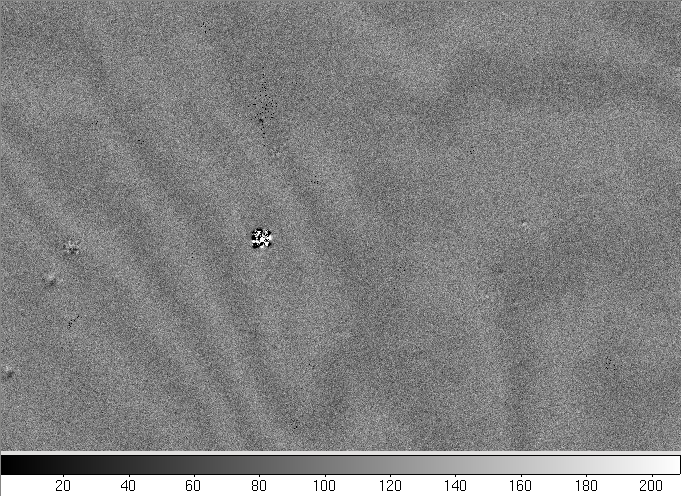
\includegraphics[width=6in]{images/rlp1233_v695833-e0-c001-a03-fom_img.png}
\caption{A figure-of-merit image for
  rlp1233/695833-e0-c001-a03}  
\label{fig:diffim2}
\end{center}
\end{figure}

\begin{figure}[htb]
\begin{center}
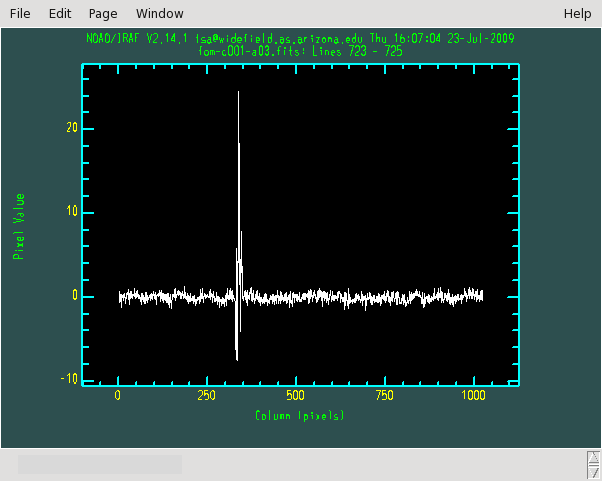
\includegraphics[width=6in]{images/rlp1233_v695833-e0-c001-a03-fom_plot.png}
\caption{Line section through figure-of-merit image for
  rlp1233/695833-e0-c001-a03.  The line is chosen to pass through the
  subtracted bright star at (338,725), which is near the center of the
image in Figure \ref{fig:diffim2}}  
\label{fig:diffim3}
\end{center}
\end{figure}

\paragraph{Difference Light Curve Quality}
Leaving out images that had WCS failures, run rlp1233 yielded 63000
objects with difference sources detected above threshold in at least
one visit. As Figure \ref{fig:lightcurve1} shows, the number of visits
for which difference sources were detected varies widely with the object, between 1 and
about 75.  The latter number is close to the number of visits
processed in rlp1233, which is 85.  Spot checking of these sources in
the images suggests that the vast majority are the result of artifacts
in the difference images, with residuals around bright stars being the
most frequent cause.  The highly structured nature of the difference
image residuals, combined with the relatively large kernel footprint,
causes further artifacts, since multiple peaks can be detected in a
single footprint.  In general, though it will certainly be the case
that real astrophysical signals from variable stars and transient
events are present in this data, it is currently impractical to
separate them from the noise with the analysis tools readily
available.

\begin{figure}[htb]
\begin{center}
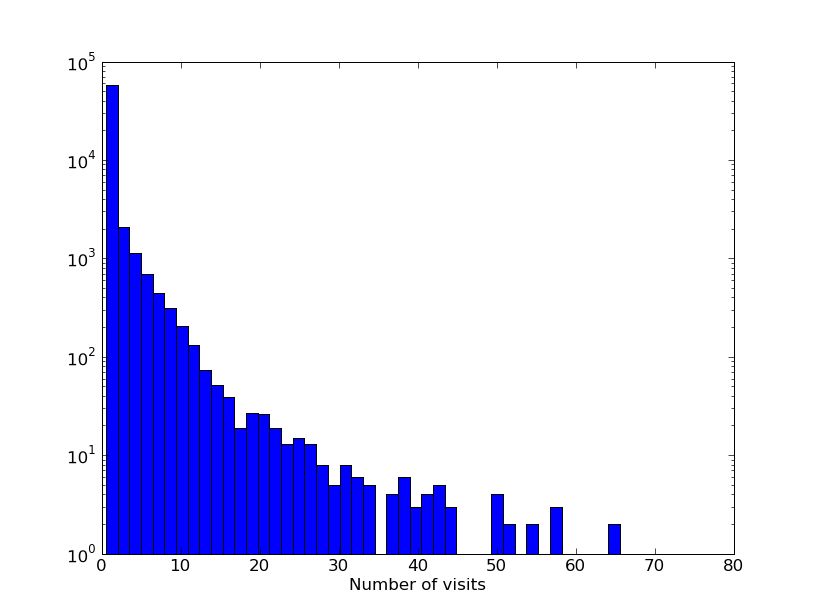
\includegraphics[width=6in]{images/rlp1233DiffLCHisto.png}
\caption{Histogram of number of Objects with DIASources in a given number of
  visits in rlp1233}  
\label{fig:lightcurve1}
\end{center}
\end{figure}

  
\paragraph{Recovery of Known Solar system Objects}

\subsection{Timing Results}
\label{sec:timing}

As in DC2, we use the logging framework (in which every log message is
time-stamped) to instrument our pipeline processing code.  We can
calculate how much time is spent on the different contributors to the
overall processing time, including I/O, middleware overhead,
scientific processing.  

\begin{table}[ht]
\begin{center}
\caption{Average Processing Times Per Visit
\label{tbl:visitstats}}
\vspace{\baselineskip}
\begin{tabular}{ l | c | c |}
\hline\hline
          & Total Processing Time, corrected
          & Application Processing Time \\ 
Pipeline  & average $\pm$  $3\sigma$ (s) & average $\pm$ $3\sigma$ (s) \\ \hline
IPSD      & 264.7 $\pm$ 20.2 & 264.1 $\pm$ 20.1  \\ 
nightmops & 10.6  $\pm$  4.4 & 0.174 $\pm$  4.4  \\ 
ap        & 1.4   $\pm$  0.7 & 0.021 $\pm$  0.7  \\ \hline
\hline
\end{tabular}

\end{center}
\end{table}


In table \ref{tbl:visitstats}, we summarize the statistics for processing
a single visit through each pipeline.  For each quantity, the error
given represents the calculated $3\sigma$ variation of the
distribution of values.  The total time is corrected to remove the
time the pipelines spend waiting for data events to arrive.  For the
IPSD and nightmops pipelines, this is the time it waits for a new data
event to arrive.  As mentioned in section \ref{brokerprob}, we
throttled the time between to data events to match the expected visit
nnprocessing time to avoid having too many unconsumed data events pile
up in the event broker; this typically resulted in an extra 20-30
second wait for a data event before processing could resume.  The ap
pipeline, on the other hand, receives its initial event from the IPSD
pipeline; thus, it had to wait on average 4.4 minutes for the IPSD
pipeline to complete before it could do its work.

\begin{figure}[htbp]
\begin{center}
%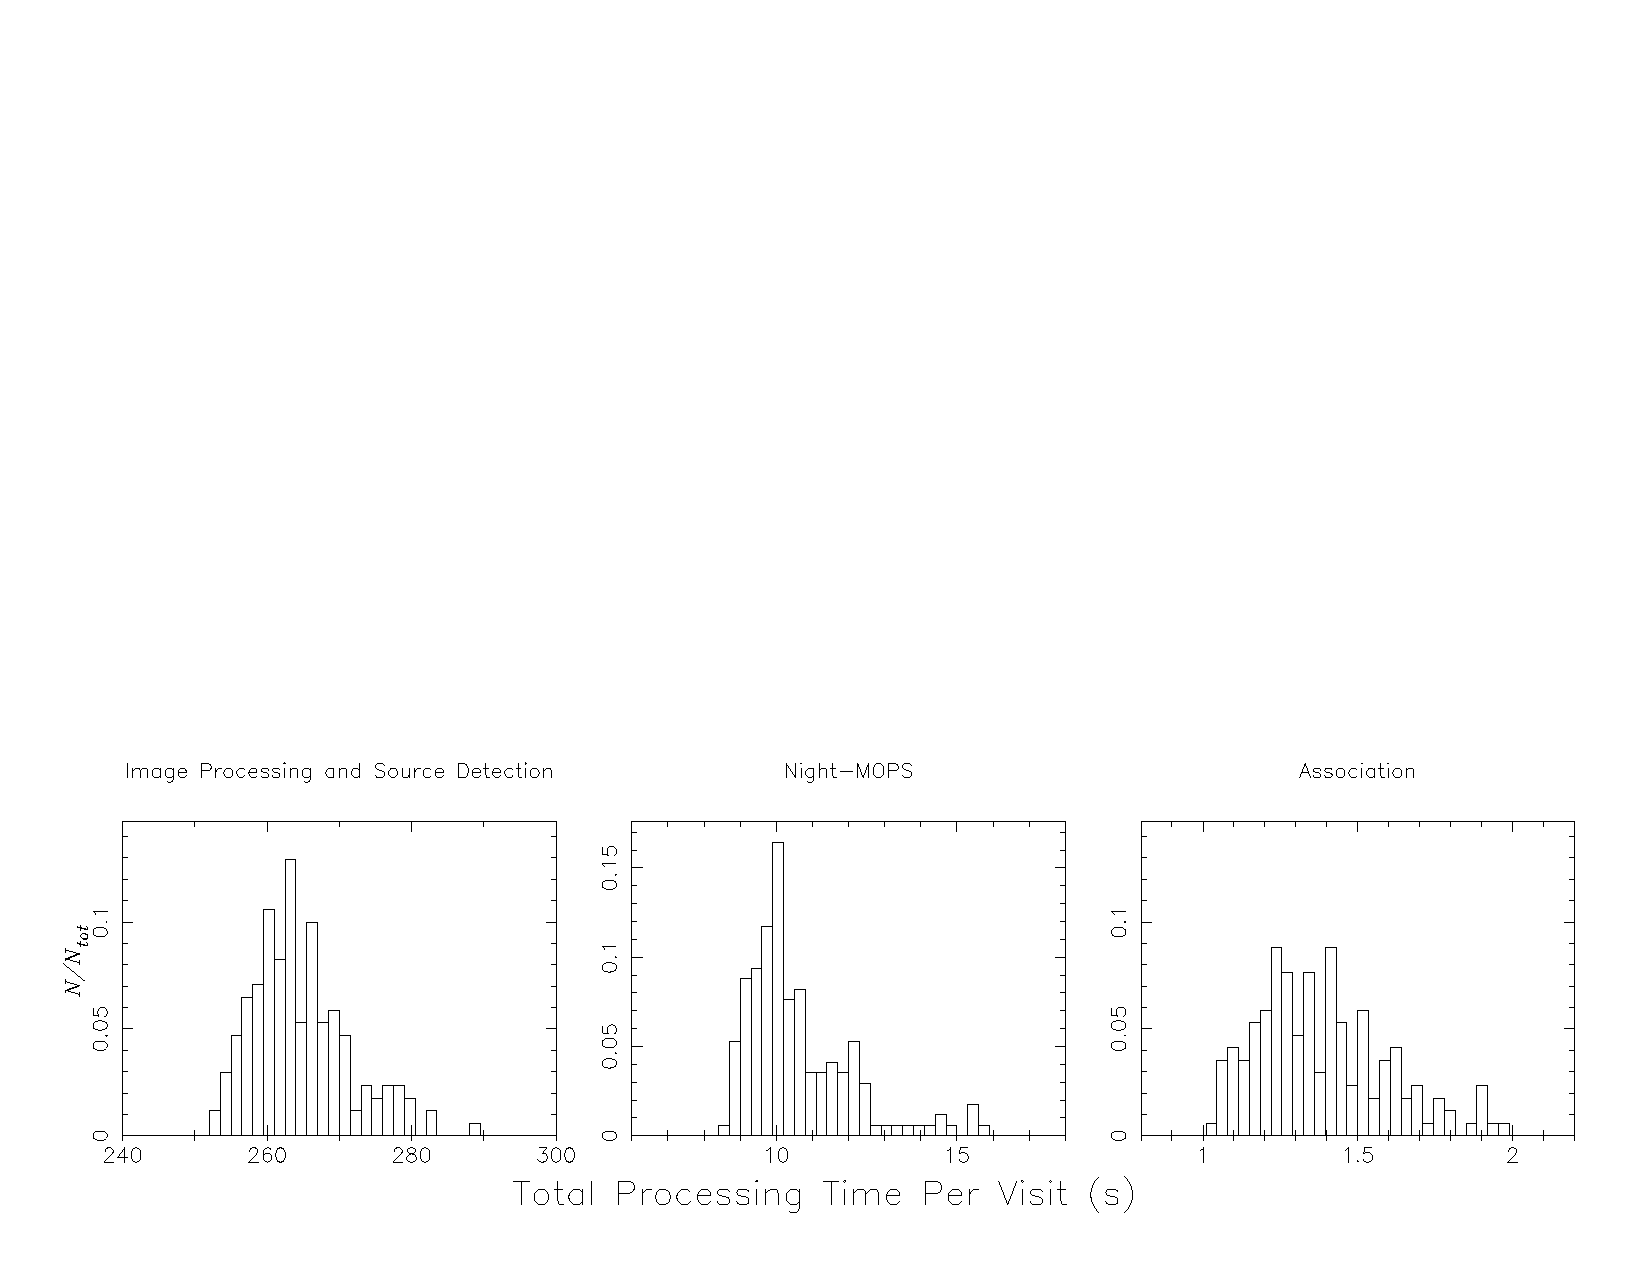
\includegraphics[width=\textwidth,bb=0 0 800 276,viewport=25 25 775 250,clip]{images/visitdist.pdf}
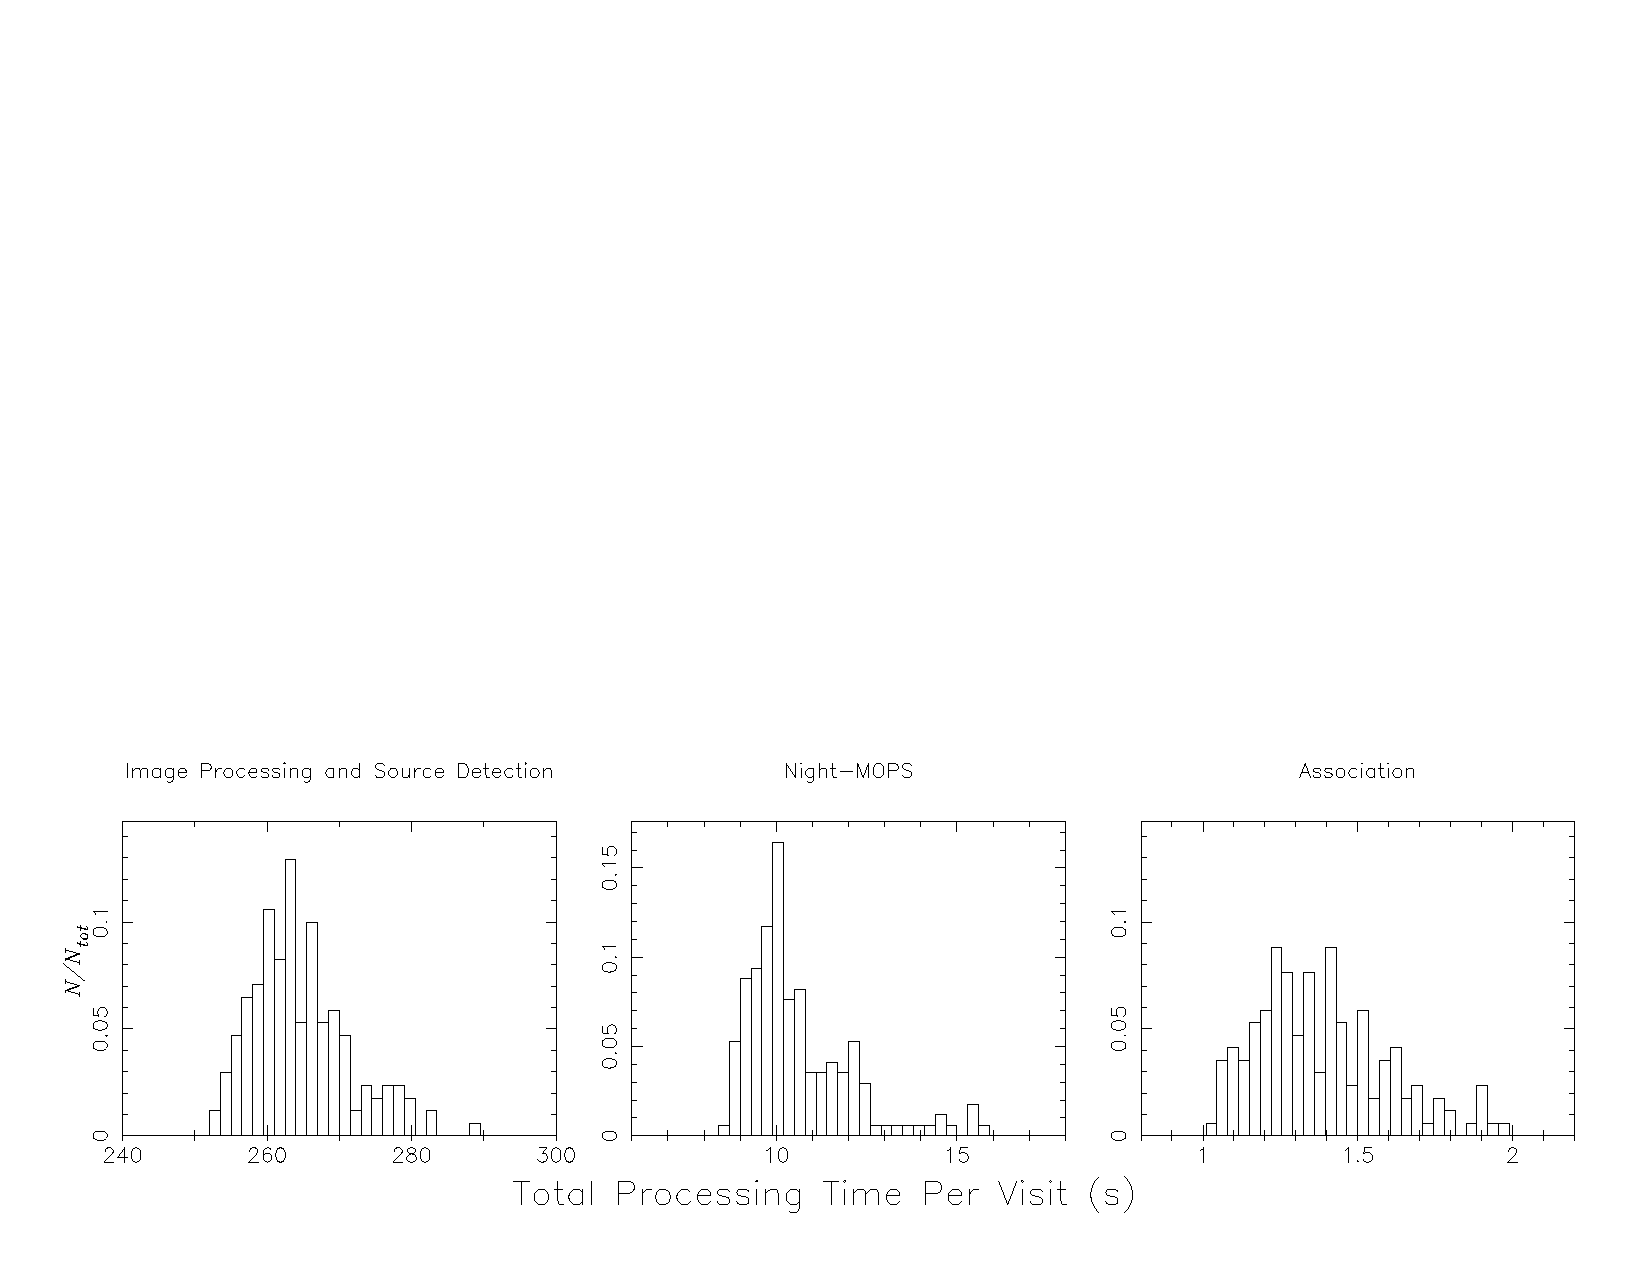
\includegraphics[width=\textwidth]{images/visitdist.pdf}
\caption{Histogram of the times to process each visit (not including
  time waiting on data events).  The $y$-axis measure the fraction of
  the 170 visits in each time bin.  
\label{fig:visitdist}}
\end{center}
\end{figure}


The ``Application Processing Time'' tallies on the time spent in total
by all the pipeline stages in their preprocess, process, and
postprocess functions where I/O is carried out and application
algorithms are applied.  (The times in these functions are included
only in cases where a stage actually provides an implementations for
them.)  It excludes the overhead by the pipeline framework for
managing the execution of the stages.  As the numbers show, the
pipeline adds very little to the processing time of a visit.  A more
precise analysis of the pipeline overhead is presented below.  

The variation in the processing is in general much smaller in DC3a as
it was in DC2: in the latter, the $3\sigma$ half-width was 108
seconds in the image processing pipeline, while we now have 20
seconds.  Furthermore as illustrated in Fig. \ref{fig:visitdist}, the
processing times do not feature the unexplained double-peaked
distributions we saw in DC2.  In summary, our we're getting much more
consistent processing times in DC3a than we did in DC2.  This has an
important impact on the overall performance because the total time
spent on a stage is driven primarily by the duration of the slice that
took the longest time.  

Tables \ref{tbl:ipsdstages} and \ref{tbl:otherstages} list the average
time spent in actual {\it application code} each stage for each pipeline.
(That is, these include the time spent in the {\tt preprocess()}, 
{\tt process()}, and {\tt postprocess()} functions only when these
were provided by a stage implementation.)  The type (``tp'') column
indicates the type of processing done by each stage, differentiating
between file-based I/O, database I/O, and the application of a
scientific algorithm.  

\begin{table}[htbp]
\begin{center}
\caption{IPSD: Average Processing Times (s) Per Stage for {\tt
    rlp1233, rlp1234} and {\tt rlpabe041}
\label{tbl:ipsdstages}}
\small
\vspace{\baselineskip}
\begin{tabular}{lrlcrrc|crr}
\hline\hline
   &    &      && \multicolumn{2}{c}{{\tt rlp1233} \& {\tt rlp1234}} 
              &&& \multicolumn{2}{c}{{\tt rlpabe041}} \\
\# & tp & Name && \multicolumn{1}{c}{average}&\multicolumn{1}{c}{$3\sigma$} 
              &&& \multicolumn{1}{c}{average}&\multicolumn{1}{c}{$3\sigma$} \\ 
\hline
 1 &    &                     sliceInfo &&  0.002 &  0.001 &&&  0.001 &  0.002 \\
 2 &    &                       symLink &&  0.001 &  0.001 &&&  0.001 &  0.002 \\
 3 &  I &                   imageInput0 &&  1.804 &  0.527 &&&  1.457 &  1.177 \\
 4 & *  &                visitMetadata0 &&  0.076 &  0.975 &&&  9.640 &  3.985 \\
 5 &    &            transformMetadata0 &&  0.013 &  0.007 &&&  0.024 &  0.122 \\
 6 &    &             validateMetadata0 &&  0.002 &  0.001 &&&  0.002 &  0.003 \\
 7 &  I &          visitMetadataOutput0 &&  0.001 &  0.001 &&&  0.001 &  0.002 \\
 8 &  I &    rawImageAndMetadataOutput0 &&  1.999 &  0.374 &&&  0.629 &  0.790 \\
 9 & *  &   identifyCalibrationProducts &&  0.020 &  0.008 &&&  0.024 &  0.036 \\
10 & *I &              calibrationInput && 11.927 &  2.810 &&&  4.453 &  3.566 \\
11 &    &  transformCalibrationMetadata &&  0.004 &  0.003 &&&  0.004 &  0.004 \\
12 & *S &                          isr0 &&  1.604 &  0.135 &&&  1.571 &  0.664 \\  % 0
13 & *S &               sourceDetection &&  1.685 &  0.449 &&&  1.695 &  1.992 \\  % 0
14 &  I &    calibAndBkgdExposureOutput && 10.627 &  1.536 &&&  3.145 &  2.595 \\
15 &  S &             sourceMeasurement &&  1.093 &  2.028 &&&  3.155 &  5.759 \\  % +
16 & *I &   exposureAndWcsSourcesOutput &&  0.228 &  0.245 &&& 11.075 & 10.217 \\
17 & *S &              psfDetermination &&  0.207 &  0.149 &&&  0.212 &  0.141 \\  % 0
18 &  I &                     psfOutput &&  0.120 &  0.097 &&&  0.121 &  0.081 \\
19 &  I &                   imageInput1 &&  1.761 &  0.494 &&&  1.693 &  1.624 \\
20 &    &                visitMetadata1 &&  0.038 &  0.033 &&& 10.039 &  0.004 \\
21 &    &            transformMetadata1 &&  0.013 &  0.005 &&&  0.011 &  0.007 \\
22 &    &             validateMetadata1 &&  0.002 &  0.002 &&&  0.001 &  0.001 \\
23 &  I &          visitMetadataOutput1 &&  0.002 &  0.002 &&&  0.001 &  0.001 \\
24 &  I &    rawImageAndMetadataOutput1 &&  2.126 &  0.553 &&&  0.910 &  1.317 \\
25 & *S &                          isr1 &&  1.709 &  0.466 &&&  1.633 &  0.596 \\  % 0
26 & *I &               wcsSourcesInput &&  0.034 &  0.029 &&& 10.045 &  0.034 \\
27 & *S &              wcsDetermination &&  0.194 &  0.050 &&&  0.249 &  0.506 \\  % +
28 & *I &     calibratedExposuresOutput && 10.514 &  1.819 &&& 11.000 &  6.178 \\
29 & *  &              CcdMetadataStage &&  0.002 &  0.001 &&&  0.003 &  0.024 \\
30 & *I &         templateMetadataInput &&  0.062 &  0.089 &&&  0.432 &  1.181 \\
31 & *  &             templateDimension &&  0.016 &  0.005 &&&  0.033 &  0.007 \\
32 & *  &                  templateBBox &&  0.004 &  0.001 &&&  0.030 &  0.192 \\
33 & *I &         templateSubimageInput && 27.218 &  3.925 &&& 57.291 & 34.928 \\
34 &  I &        templateSubimageOutput &&  5.574 &  1.043 &&&  2.209 &  1.212 \\
35 & *S &              imageDifference0 && 82.343 &  9.706 &&& 77.912 &  5.336 \\  % -
36 & *S &              imageDifference1 && 80.247 & 11.998 &&& 75.806 &  8.876 \\  % -
37 & *I &         differenceImageOutput && 10.172 &  1.606 &&&  3.260 &  2.316 \\
38 & *S &                  addAndDetect &&  7.966 &  0.126 &&& 12.335 &  2.423 \\  % +
39 & *S &          diaSourceMeasurement &&  0.473 &  2.211 &&&  7.830 & 23.511 \\  % +
40 & *  &             sourceToDiaSource &&  0.050 &  0.082 &&&  0.125 &  0.109 \\
41 & *S &          sourceClassification &&  0.008 &  0.007 &&&  0.059 &  0.405 \\  % +
42 & *I &              diaSourceOutput0 &&  1.947 &  4.220 &&& 10.210 &  0.232 \\
43 & *I &              diaSourceOutput1 &&  0.106 &  0.143 &&& 10.206 &  0.182 \\
44 & *  &              associationEvent &&  0.002 &  0.001 &&&  0.001 &  0.001 \\
45 & *I &                   sdqaOutput0 &&  0.047 &  0.015 &&& 10.056 &  0.012 \\
46 & *I &                   sdqaOutput1 &&  0.028 &  0.010 &&& 10.050 &  0.170 \\
\hline
\multicolumn{10}{l}{Type codes: FI = input/output stage, * = production stage,
S = scientific algorithm stage} \\
\end{tabular}
\end{center}
\end{table}

As in DC2, the costliest stages are those that do image subraction
(stages 35 and 36) at 80 seconds per image.  This is down
significantly from DC2's 175 seconds; although, in DC3 we now do image
subtraction on both exposures from a visit.  The variation in the time
is down considerably as well.  One of the tunable parameters we found
that can have a significant effect on the subtraction time is the 
{\tt maxPrincipalComponents} policy parameter, which controls the number
of principal components calculated for the ... step and which in this
run was set to 10.  We believe that we can probably reduce this
parameter to 5 without loss in processing fidelity; subsequent tests
with this value ({\tt rlp1248}) indicate that this would reduce the
duration of the image subtraction stage by another 20 seconds.

\begin{table}[htbp]
\begin{center}
\small
\caption{Night-MOPS and Association: Average Processing Times (s) Per
  Stage.
\label{tbl:otherstages}}
\vspace{\baselineskip}
\begin{tabular}{lrlrr|lrlrr}
\hline\hline
\multicolumn{5}{c|}{Association} & \multicolumn{5}{c}{Night-MOPS} \\
\# & tp & Name & \multicolumn{1}{c}{average}&\multicolumn{1}{c|}{$3\sigma$} &
\# & tp & Name & \multicolumn{1}{c}{average}&\multicolumn{1}{c}{$3\sigma$} \\ 
\hline
1 &    & symLink                  &  0.001 &  0.006 & 1 & *S & NightMopsStage           & 10.228 &  4.485 \\ 
2 &  I & load                     &  0.458 &  0.081 & 2 & *I & output                   &  0.155 &  0.597 \\ 
3 & *I & diaSourceInput           &  0.015 &  0.017 & 3 & *\phantom{I}  & associationEvent         &  0.020 &  0.078 \\ 
4 & *S & MatchDiaSourcesStage     &  0.005 &  0.005 &&&&&\\ 
5 & *S & diaSourceMatchOutput     &  0.259 &  0.406 &&&&&\\ 
6 & *I & predInput                &  0.003 &  0.004 &&&&&\\ 
7 & *S & MatchMopsPredsStage      &  0.002 &  0.002 &&&&&\\ 
8 & *I & predMatchAndObjectOutput &  0.112 &  0.231 &&&&&\\ 
9 & *I & store                    &  0.379 &  0.248 &&&&&\\ 
\hline
\multicolumn{10}{l}{Type codes: I = input/output stage, S = Stage
  applying a scientific algorithm, * = production stage,} \\
\multicolumn{5}{l}{} \\
\end{tabular}
\end{center}
\end{table}

Comparing the LSST cluster runs with the Abe run reveals how the IPSD 
pipeline holds up to scaling.  Note that the Abe run processed 9 times
more data.  Of the 11 science stages, we see that for four of them,
the average processing time was the same within one sigma.  For five
of them, the time went up significantly.  However, for the two most
expensive stages--image subtraction--the time went down.  In general,
the variation in the average times went up.  We again note that for
the IPSD pipeline the time spent in each stage is essentially the time
of the longest-running slice in a visit.  

Based on these times, we might conclude that the stages where
processing times did not change demonstrate near perfect scaling; that
is, the processing time does not change as we add more data onto more
nodes.  However, the improvement we see in the image subtraction
stages perhaps reflect hardware differences such as Abe's slightly
faster processors (2.33 GHz versus 2.0 GHz) or increased available
memory (8 GB per node versus 4 GB).  This better hardware could also
be benefitting all stages.  To discern the contribution made by the
better hardware, we would need to compare these results with
smaller-scale runs--i.e. 31 slices--on Abe.  Nevertheless, relative
gain for images subtraction is modest--$\sim 5\%$--which is comparable
to the one-sigma variation for the shorter science stages and, thus,
would not make a big difference.  The remaining science stages do show
a degredation in the scaling.  

Since the times above reflect the slowest slice in a stage, we might
expect these times to go up since by exploring more data, we should
expect to sample more challenging data that require more processing
time and consequently slow down the processing of an entire visit.  To
understand the scaling of the underlying algorithm, it is perhaps
better to not look at the distribution in the slowest slices in a
visit but rather in all of the slices over all of the visits.  This
appears in table \ref{tbl:allscislices}.  The last column expresses
the difference in terms of the oft-cited speed-up factor (where 1
represents perfect linear speed-up).  The values larger than 1 are
presumably due to Abe's better hardware.  In these statistics
illustrate very good scaling for most of the science stages.  In only 
only three of the stages ({\tt addAndDetect, diaSourceMeasurement,}
and {\tt sourceClassification}) do we see some degredation.  The
reasons for this are unclear at this point and thus will warrant more
testing.  

\begin{table}[htbp]
\begin{center}
\caption{IPSD: Average Processing Times (s) Per Stage across all
  Slices and Visits
\label{tbl:allscislices}}
\vspace{\baselineskip}
\begin{tabular}{llcrrc|crr|c}
\hline\hline
   &      && \multicolumn{2}{c}{{\tt rlp1233} \& {\tt rlp1234}} 
         &&& \multicolumn{2}{c|}{{\tt rlpabe041}} & \\
\# & Name && \multicolumn{1}{c}{average}&\multicolumn{1}{c}{$3\sigma$} 
         &&& \multicolumn{1}{c}{average}&\multicolumn{1}{c|}{$3\sigma$} 
   & Speed-up \\ 
\hline
12 &                 isr0 &&  1.514 &  0.113 &&&  1.389 &  0.275 & 1.1 \\  % -
13 &      sourceDetection &&  1.638 &  0.110 &&&  1.479 &  0.465 & 1.1 \\  % - 
15 &    sourceMeasurement &&  0.232 &  0.772 &&&  0.234 &  1.184 & 1.0 \\  % 0 
17 &     psfDetermination &&  0.112 &  0.120 &&&  0.107 &  0.123 & 0.9 \\  % 0 
25 &                 isr1 &&  1.585 &  0.163 &&&  1.439 &  0.184 & 1.1 \\  % 0 
27 &     wcsDetermination &&  0.172 &  0.085 &&&  0.191 &  0.403 & 0.9 \\  % 0 
35 &     imageDifference0 && 71.174 & 15.573 &&& 62.082 & 14.898 & 1.1 \\  % - 
36 &     imageDifference1 && 69.289 & 15.198 &&& 61.069 & 15.717 & 1.1 \\  % - 
38 &         addAndDetect &&  7.851 &  0.680 &&&  9.354 &  3.400 & 0.6 \\  % + 
39 & diaSourceMeasurement &&  0.114 &  0.610 &&&  0.261 &  2.979 & 0.4 \\  % + 
41 & sourceClassification &&  0.005 &  0.005 &&&  0.008 &  0.029 & 0.8 \\  % + 
\hline
\end{tabular}
\end{center}
\end{table}

Data input and output (I/O) takes on average 46\% of the time spent
processing a visit in the IPSD pipeline (or 24\% if we discount
non-essential I/O).  Comparison of the LSST cluster runs ({\tt
rlp1233} \& {\tt rlp1234}) with the Abe run is revealing, particularly
when we break it differentiate between file-based I/O and database
I/O.  






% -- Section 8
% Section 8: Conclusions

\section{Conclusions}

We draw the following conclusions from the results of Data Challenge 3a.

\begin{itemize}

\item Production runs show improvements in DC3a in execution time for common
stages of the IPSD pipeline when compared to DC2. Additional improvement of
execution time is not scoped for DC3b, but will be a major priority for DC4. We
cannot assume that Moore's Law will solve the performance problem for us. We
continue to believe that the processing times necessary for full production
throughput during real-time operation will be reached, but recognize that this
will require considerable attention in DC4.

\item Source detection now is hampered by the quality of the image subtractions.
Registration errors between the calibrated exposure images and the corresponding
template need to be improved; currently misalignment leads to artifacts which
result in many false source detections, along with very strong spurious peaks in
the resulting lightcurves. DC3b will include improvement of the science data
quality as a major focus.

\item Tests on the Abe cluster showed that the pipelines scaled reasonably 
well when applied to the entire focal plane of a CFHT-LS exposure. The 
pipeline stage harness supporting the science algorithms was designed to
be computationally lightweight, and analysis of runs on Abe show that 
comparatively little processing time is spent by this infrastructure.

\item Early in DC3, the code tree underwent significant refactoring and was
additionally upgraded for 64-bit support. These steps were important and
necessary, but left developers without the ability to test implementations
inside the harness framework until comparatively late in the DC3a development
cycle. DC3b will use several strategies, including continuous integration
and additional tools for running science stages independently from the 
LSST cluster.

\end{itemize}

% -- References
\begin{thebibliography}{}

\bibitem[Borne {\it et al.}(2009)]{borne09} Borne, K. D., R. Laher, Z. Ivezic, and N. Hamam 2009,
   Petascale Object Classification of the LSST Event Stream, 
   Poster presented at the 213th AAS Meeting, Long Beach, CA, 4-8 January 2009.

\bibitem[Laher {\it et al.}(2008)]{laher08} Laher, Russ R., Deborah Levine, Vince Mannings, 
   Peregrine McGehee, Jeonghee Rho, Richard A. Shaw, and Jeff Kantor 2008,
   LSST Science Data Quality Analysis Subsystem Design,
   Oral presentation given at the ADASS XVIII Conference, Quebec City, Ontario, Canada, 
   2-5 November 2008.

\bibitem[Press et al., 2007]{PressNR}
W.~H. Press,  S.~A. Teukolsky, W.~T. Vetterling, B.~P. Flannery.
Numerical Recipes: the Art of Scientific Computing.
2007, Cambridge University Press.
   
\end{thebibliography}



\end {document}


